\documentclass{easychair}
%\usepackage{rotating}
%\usepackage{pdflscape}
%usepackage{algorithm2e}
\newcommand{\easychair}{\sf{easychair}}
\newcommand{\miktex}{MiK{\TeX}}
\newcommand{\texniccenter}{{\TeX}nicCenter}
\newcommand{\makefile}{\texttt{Makefile}}
\usepackage[portuguese]{babel}
\usepackage{epsfig}
\usepackage{subfig,syntonly,amsmath,amssymb,cite,graphicx}
\usepackage{nomencl}
\usepackage[strings]{underscore}
\usepackage{float}
\usepackage{amsthm}
\usepackage{amsmath}
\usepackage{array}

\usepackage{caption}
\usepackage{subcaption}
\usepackage{subfig}


%\usepackage[utf8]{inputenc}  % adaptar 'a codificacao do sistema
%\usepackage[portuges]{babel}

%% Document
%%
\begin{document}
\raggedbottom

\title{Segmentação de Clientes e Previsão do Risco de Abandono Através de Análise RFM}

\titlerunning{}

% Authors are joined by \and and their affiliations are on the
% subsequent lines separated by \\ just like the article class
% allows.
%

\author{Rui Ruivo\\
Universidade de Évora\\
\url{m60739@alunos.uevora.pt}\\
}

\authorrunning{R. Ruivo}

\maketitle

%----------------------------------------------------------------------------------------------------------
\begin{abstract}
O aumento exponencial das plataformas de \textit{e-commerce} transformou os comportamentos de consumo, exigindo que as organizações desenvolvam estratégias centradas no cliente para maximizar a retenção e reduzir o risco de abandono. Este estudo explora a utilização da análise RFM (\textbf{Recência}, \textbf{Frequência} e \textbf{Valor Monetário}) como uma ferramenta de segmentação de clientes e cálculo do risco de abandono, utilizando o conjunto de dados "\textbf{Online Retail II}" \cite{dataset}.

Inicialmente, o conjunto de dados foi preparado por meio da limpeza e normalização dos valores RFM, aplicando técnicas como \textit{equal-frequency binning} para minimizar o impacto de outliers. A segmentação foi realizada por \textit{K-means clustering}, com a seleção do número ideal de clusters feita através do método do cotovelo (\textit{Elbow Method}). Adicionalmente, foi desenvolvido um modelo para calcular a probabilidade de abandono dos clientes com base em uma combinação ponderada das métricas RFM, fornecendo \textit{insights} detalhados sobre os níveis de risco.

Os segmentos de clientes identificados incluíram grupos como clientes VIP, clientes fiéis, grandes gastadores ocasionais, clientes em risco e clientes perdidos, permitindo uma análise detalhada das suas características comportamentais. A visualização tridimensional dos \textit{clusters} destacou padrões relevantes, facilitando a identificação das zonas críticas de abandono.

Para validar os resultados, foram utilizados algoritmos de classificação como \textit{J48}, \textit{Random Forest}, Regressão Logística (\textit{Logistic}), \textit{SMO} e \textit{IBk}. Os classificadores foram avaliados por meio de uma análise da curva de aprendizagem, garantindo resultados robustos e minimizando o risco de \textit{overfitting}.

Embora o estudo se concentre exclusivamente nas métricas RFM, os resultados demonstram a eficácia dessas abordagens para a compreensão do comportamento do cliente e a previsão de abandono. A inclusão de variáveis adicionais, como características demográficas e socioeconômicas, é recomendada como trabalho futuro para melhorar ainda mais a precisão dos modelos. Este trabalho fornece uma base metodológica sólida para empresas que buscam implementar estratégias baseadas em dados para retenção e fidelização de clientes.
\end{abstract}
%----------------------------------------------------------------------------------------------------------

%----------------------------------------------------------------------------------------------------------
\section{Introdução}
Com o aparecimento da Internet, principalmente aquando da sua massificação no íncio dos anos 2000, houve uma mudança de paradigma na forma como as pessoas realizavam compras. Se até aí a realização de compras implicava a deslocação a uma loja ou a uma grande superfície comercial (o que se traduzia num aumento de custos, como despesas com combustível e a perda de tempo associada à deslocação), a Internet permitiu o aparecimento de plataformas de \textit{E-commerce} que ofereciam aos utilizadores a possibilidade de realização de compras dos mais variados artigos sem que tivessem de sair de casa.

De acordo com dados do \textit{Eurostat}, entre 2010 e 2023 houve um aumento de 22\% no número de utilizadores que compraram ou encomendaram bens ou serviços no último ano\cite{eurostat}. Esse crescimento, aliado a inovações tecnológicas como os \textit{smartphones}, \textit{apps} e pagamentos online seguros, influenciou os comportamentos de consumo e preferências dos utilizadores.

Neste novo mundo de rápida evolução tecnológica, torna-se necessário que as organizações adotem técnicas que lhes permitam compreender os comportamentos dos consumidores, identificando não só os seus clientes mais valiosos, mas também quais os clientes que se encontram em risco de deixar de usar os seus serviços, cancelar uma assinatura ou simplesmente parar de fazer compras. Felizmente para as organizações, a interação dos seus clientes com os seus serviços deixa uma riqueza de dados que podem ser explorados para caracterizar os seus hábitos e ajudar a definir estratégias personalizadas para aumentar não só a retenção, fidelização e o lucro, mas também a criação de novos produtos que vão ao encontro dos gostos dos clientes.

Para solucionar este problema, foi realizada pesquisa sobre este tema e sobre as principais abordagens já publicadas. Um dos artigos mais interessantes é intitulado de \textit{\textbf{"Visualizing RFM Segmentation"}}\cite{RFMSDM2004} da autoria de \textit{Ron Kohavi} e \textit{Rajesh Parekh}. Neste artigo, os autores discutem as técnicas mais utilizadas para a realização de segmentação de clientes com base na análise RFM, e apresentam os resultados em gráficos 2D e 3D de fácil interpretação.

Outro artigo, que utiliza o conjunto de dados \textit{"Online Retail II"}\cite{dataset} que também irá ser analisado neste artigo, é intitulado de \textit{\textbf{"Data mining for the online retail industry: A case study of RFM model-based customer segmentation using data mining"}} da autoria de \textit{Daqing Chen}, \textit{Sai Laing Sain} e \textit{Kun Guo}. Neste artigo, os autores discutem a utilização de algoritmos de \textit{clustering} como \textit{K-means clustering} além de árvores de decisão para refinar a segmentação de clientes através das métricas RFM.

O último artigo a apresentar é intitulado de \textit{\textbf{"Retail Customer Churn Analysis using RFM Model and K-Means Clustering"}} da autoria de \textit{Nikita Bagul}, \textit{Prerana Berad}, \textit{Prof. Priya Surana} e \textit{Chirag Khachane}. Neste artigo, é utilizado o conjunto de dados \textit{"Online Retail"}\cite{dataset2}, que consiste num \textit{subset} do conjunto de dados que iremos analisar de seguida com dados de Dezembro de 2010 a Dezembro de 2011, os autores discutem os passos necessários para a preparação do \textit{dataset} para que se possa aplicar a análise RFM e a segmentação de clientes com base em \textit{K-means Clustering}. Apresentam também uma explicação de como procederam na escolha do número adequado de clusters, através da aplicação da \textit{\textbf{Elbow Technique}}.

Com base nestes artigos, decidi realizar a minha própria análise RFM para permitir a recolha de informação para cada cliente sobre a data da sua última compra, qual a frequência com a qual o cliente interage com a organização (ou seja, quantas vezes realizou compras) e qual o valor total que o cliente gastou no conjunto de todas as suas compras, este procedimento é a base da análise RFM. Além disso, com base na pontuação RFM obtida, é feita a segmentação dos clientes em grupos através de \textit{k-means clustering}.

Um ponto em que a implementação neste artigo difere das restantes é na utilização das métricas RFM para calcular um valor normalizado de probabilidade de abandono (o chamado \textbf{\textit{customer churn}}) para cada cliente. Este cálculo irá permitir encontrar, quando realizado um plot 2D ou 3D dos resultados, zonas do gráfico onde a probabilidade de abandono é alta, mesmo quando esses clientes são segmentados em categorias de clientes ditos de "Baixo Risco", como os melhores clientes ou os clientes leais. Pois nada indica que um cliente leal ou um dos melhores clientes não possa de futuro tornar-se inativo. Como tal, a realização deste artigo pretende dar uma maior compreensão às organizações sobre os seus clientes, bem como os riscos associados aos mesmos.


O último passo passa pela avaliação do nosso modelo através da utilização de algoritmos classificadores, como \textbf{\textit{J48}}, \textbf{\textit{Logistic}} (implementação do Weka de regressão logística), \textbf{\textit{RandomForest}}, \textbf{\textit{SMO}} e \textbf{\textit{IBk}}. A metodologia adotada, bem como os passos tomados para a preparação do conjunto de dados, serão apresentados mais à frente neste artigo.

Na realidade, a utilização apenas das componentes de Recência, Frequência e valor Monetário, embora sejam fáceis de calcular e perceber, apenas cobrem um aspeto do comportamento dos clientes. Na obtenção de modelos de previsão com alta qualidade, são necessários mais dados acerca das necessidades dos utilizadores, as suas opiniões, características socio-económicas e dados relacionais, entre outros\cite{SGEM2008}. Na realização deste estudo, iremos focar-nos na previsão do risco de abandono apenas com base nas métricas RFM, dado que o nosso conjunto de dados tem informação limitada sobre as transações de clientes por questões de privacidade dos dados. No entanto, os procedimentos realizados aqui podem ser estendidos a outros estudos, dependendo sempre da estratégia empresarial tomada por cada organização.

%----------------------------------------------------------------------------------------------------------

\newpage


%----------------------------------------------------------------------------------------------------------
\section{Conjunto de Dados escolhido}

Para a realização da tarefa proposta neste artigo, irá ser utilizado o conjunto de dados \textit{"Online Retail II"}\cite{dataset}. Este conjunto de dados consiste em registos de transações comerciais de uma plataforma de \textit{E-commerce} do Reino Unido. As transações comerciais ocorreram entre 01/12/2009 e 09/12/2011. A empresa responsável pela plataforma vende maioritariamente artigos de oferta. Muitos dos seus clientes são atacadistas (\textit{wholesalers}).

O conjunto de dados é composto por 1048124 instâncias e 8 atributos, com as seguintes características:

\begin{enumerate}
    \item \textbf{Invoice}: Atributo nominal. Número de fatura que identifica cada compra realizada por determinado cliente. As devoluções são identificadas pelo número de fatura precedido por 'C'.
    \item \textbf{StockCode}: Atributo nominal. Corresponde ao código identificador de cada artigo.
    \item \textbf{Description}: String que descreve o artigo comprado.
    \item \textbf{Quantity}: Atributo numérico. Corresponde à quantidade do artigo. Caso a fatura seja um cancelamento ou devolução, o número é negativo.
    \item \textbf{InvoiceDate}: String que indica a data da fatura.
    \item \textbf{Price}: Atributo numérico. Indica o preço por unidade do artigo comprado.
    \item \textbf{Customer}: Atributo numérico que identifica unicamente cada cliente.
    \item \textbf{Country}: Atributo nominal. Indica o país de residência do cliente.
\end{enumerate}

Este conjunto de dados não está pronto a utilizar, sendo necessária a realização da limpeza de instâncias inválidas ou com valores em falta, para minimizar os erros (\textit{outliers}) que possam ocorrer durante a análise. Esta limpeza irá ser realizada de seguida.


Todos os ficheiros utilizados na realização desta análise (desde o conjunto de dados original, o conjunto de dados final, código, dados de teste e treino e resultados de testes) poderão ser encontrados no link na bibliografia\cite{ficheiros}.

\newpage

\section{Preparação do conjunto de dados}
\subsection{Remoção das instâncias com valores em falta}

O primeiro passo na limpeza dos dados é a identificação e remoção de instâncias com valores em falta. Como o nosso objetivo final é a segmentação de clientes, devemos olhar para a coluna \textit{"Customer"} e remover todas as instâncias sem a informação relativa ao cliente. Caso se mantivesse essa informação, o agrupamento dos dados por cliente iria reunir todas as compras sem número de cliente num só registo, como se se tratasse de um cliente apenas, o que iria tornar a nossa analise menos precisa.
Para realizar a limpeza dos dados em falta, iremos utilizar o Microsoft Excel. Começamos por abrir o programa filtramos os dados vazios pela coluna \textit{"Customer ID"}. A figura \ref{fig1} mostra a aplicação do filtro:

\begin{figure}[H]
    \begin{centering}
    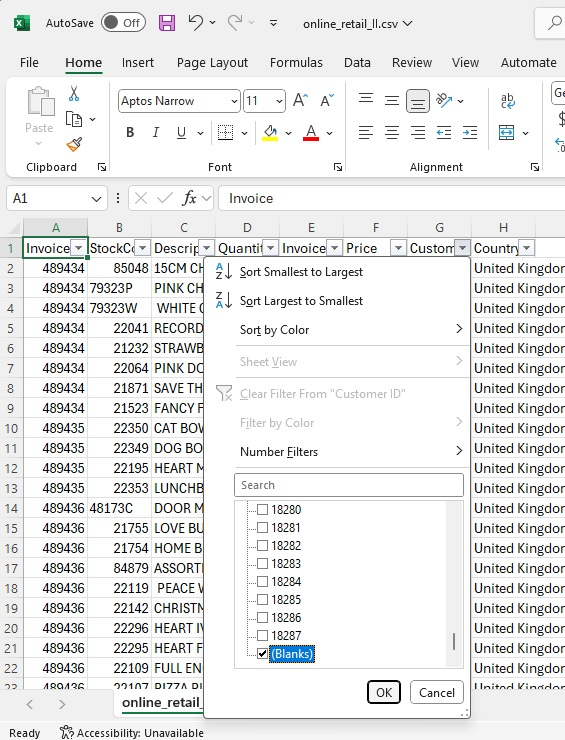
\includegraphics[width=0.55\linewidth]{imagens/figure1.jpg}\label{cap-2-fig1}
    \captionof{figure}[LOF entry]{Filtro das instâncias com \textit{"Customer ID"} vazio.}
    \label{fig1}
    \end{centering}
\end{figure}

Após filtrarmos as linhas, selecionamos todas as que queremos eliminar e clicamos em \textit{"Delete"} no teclado. O ficheiro passou das suas 1048124 instâncias para 811894 instâncias.

\newpage

\subsection{Remoção das instâncias correspondentes a cancelamentos e cálculo de valores de RFM por cliente}

De seguida, devemos eliminar também as instâncias dos nossos dados que dizem respeito a devoluções e cancelamentos de encomendas.  Para tal, utilizamos um \textit{script} Python desenvolvido para esse efeito\cite{pythonRFM}. Esse script irá também calcular os valores de Recência, Frequência e valor Monetário para cada cliente, que irão ser importantes para a análise posterior.
No fim de corrermos o \textit{script} iremos ter um ficheiro .csv com os cálculos RFM para cada cliente e sem as linhas referentes a cancelamentos.

Com a realização desta limpeza do conjunto de dados, estamos prontos a passar aos próximos passos, com o software \textit{Weka}\cite{weka}.

%----------------------------------------------------------------------------------------------------------

\subsection{Remoção de duplicados através do Weka}

Para procedermos à análise do nosso \textit{dataset}, iremos precisar de o carregar no \textit{Weka}. Para tal, depois da abertura do programa, devemos carregar no botão \textit{"Explorer"}, de seguida, clicamos no botão \textit{"Open file..."} e escolhemos qual o ficheiro abrir. Após a abertura do ficheiro, a janela do \textit{"Explorer"} deverá mostrar algo como representado na figura \ref{fig2} :

\begin{figure}[H]
    \begin{centering}
    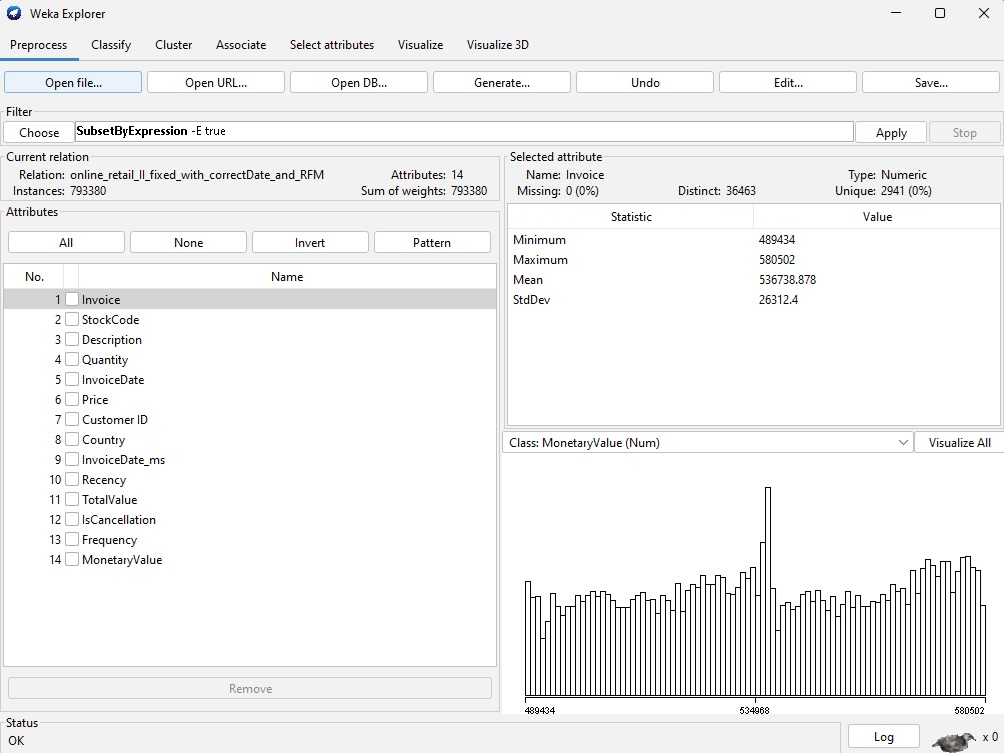
\includegraphics[width=1\linewidth]{imagens/figure2.jpg}\label{cap-2-fig2}
    \captionof{figure}[LOF entry]{Janela do Weka após o carregamento inicial do conjunto de dados.}
    \label{fig2}
    \end{centering}
\end{figure}

\vspace{-0.3cm}
Ao terminar o carregamento, podemos notar que o nosso conjunto de dados passou de 1048124 para 793380 instâncias, isto porque anteriormente foram eliminadas as instâncias com o campo \textit{"Customer ID"} vazio e as instâncias que diziam respeito a cancelamentos e devoluções. Podemos reparar que passámos de 8 para 14 atributos, mas muitos destes foram utilizados como atributos temporários pelo \textit{script} Python utilizado anteriormente por forma a calcular os valores de Recência, Frequência e Valor Monetário e como tal deverão ser removidos. Para esse efeito, iremos simplesmente selecionar os atributos a remover no \textit{Weka} e clicar no botão \textit{"Remove"} situado por debaixo da lista de atributos. A figura \ref{fig3} ilustra quais os atributos a remover:

\begin{figure}[H]
    \begin{centering}
    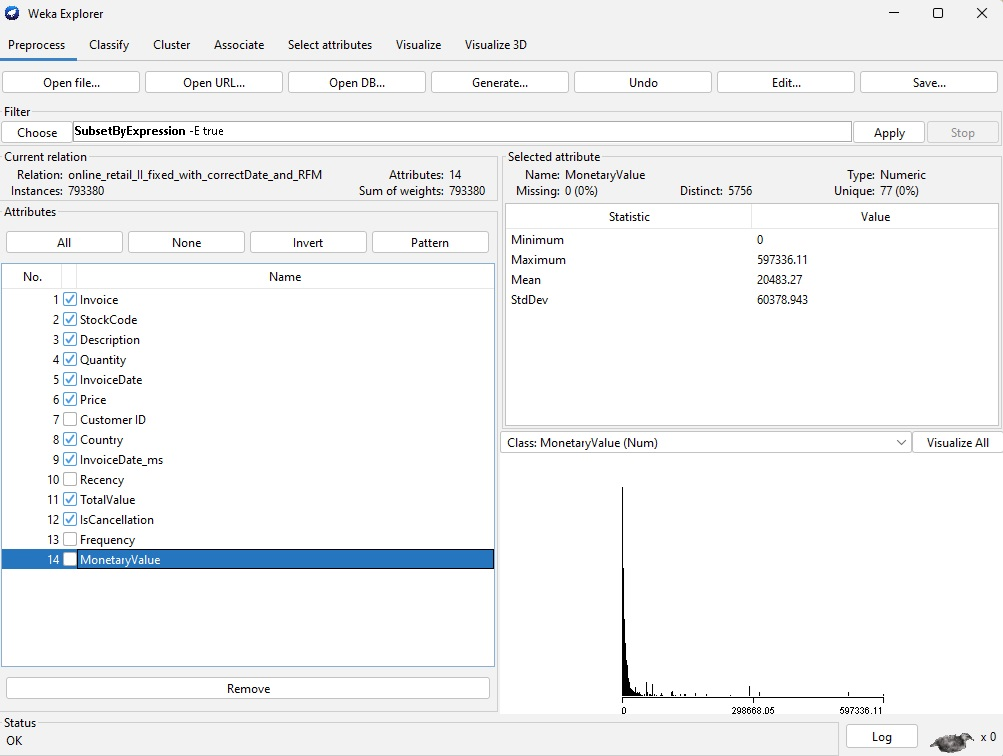
\includegraphics[width=1\linewidth]{imagens/figure3.jpg}\label{cap-2-fig3}
    \captionof{figure}[LOF entry]{Indicação dos atributos a remover do conjunto de dados}
    \label{fig3}
    \end{centering}
\end{figure}

Terminada a remoção dos nossos atributos, o próximo passo é a conversão do atributo \textit{"Customer ID"} de numérico para nominal. Para esse efeito, iremos utilizar o filtro \textit{\textbf{NumericToNominal}}, bastando nas opções do mesmo alterar o campo \textit{atributeIndices} e substituir "first-last" por apenas "first". A seguinte figura demonstra essa alteração:

\vspace{-0.2cm}
\begin{figure}[H]
    \begin{centering}
    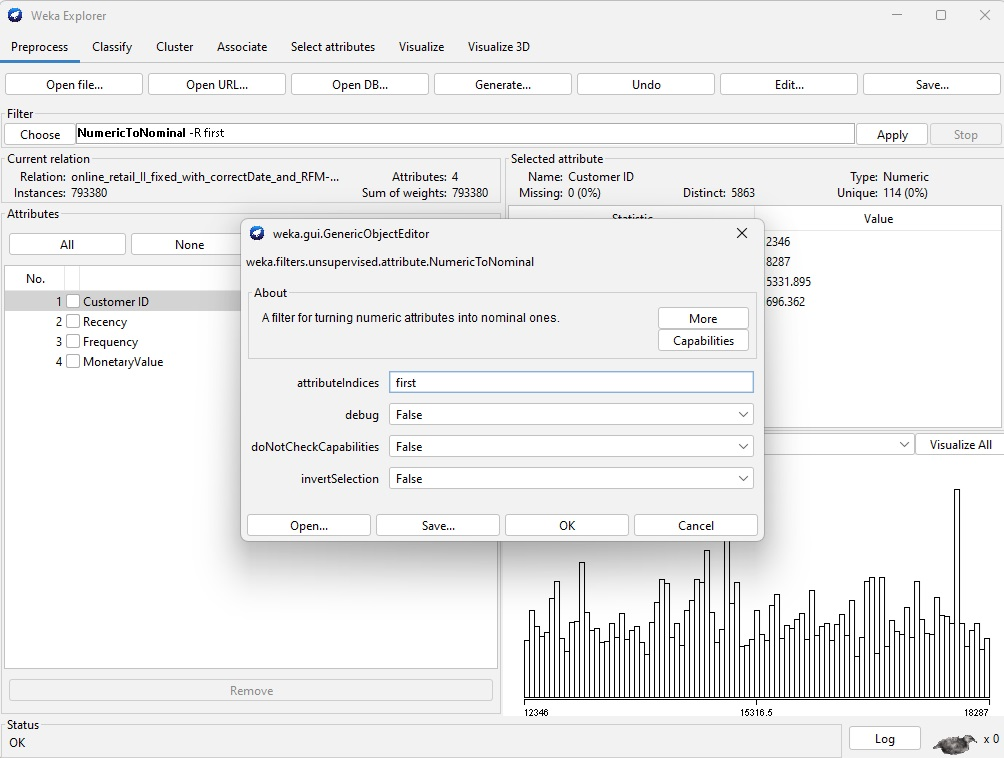
\includegraphics[width=1\linewidth]{imagens/figure4.jpg}\label{cap-2-fig4}
    \captionof{figure}[LOF entry]{Opções do filtro \textbf{\textit{NumericToNominal}}.}
    \label{fig4}
    \end{centering}
\end{figure}


\vspace{-0.3cm}
O último passo antes da análise dos dados é a remoção de duplicados. Anteriormente, quando foi feita a remoção de instâncias que diziam respeito a linhas canceladas, foram também calculados os valores de RFM. Estes valores aparecem repetidos por cada instância e por cada cliente, logo removendo os duplicados no \textit{Weka} irá deixar-nos com uma instância por cliente, com os seus valores de RFM. Para podermos realizar esse passo, iremos utilizar o filtro \textbf{\textit{RemoveDuplicates}}. Este filtro não necessita de configurações adicionais, bastando escolher o mesmo e clicar no botão \textit{"Apply"}. A figura seguinte mostra o resultado final da aplicação do filtro:

 \begin{figure}[H]
    \begin{centering}
    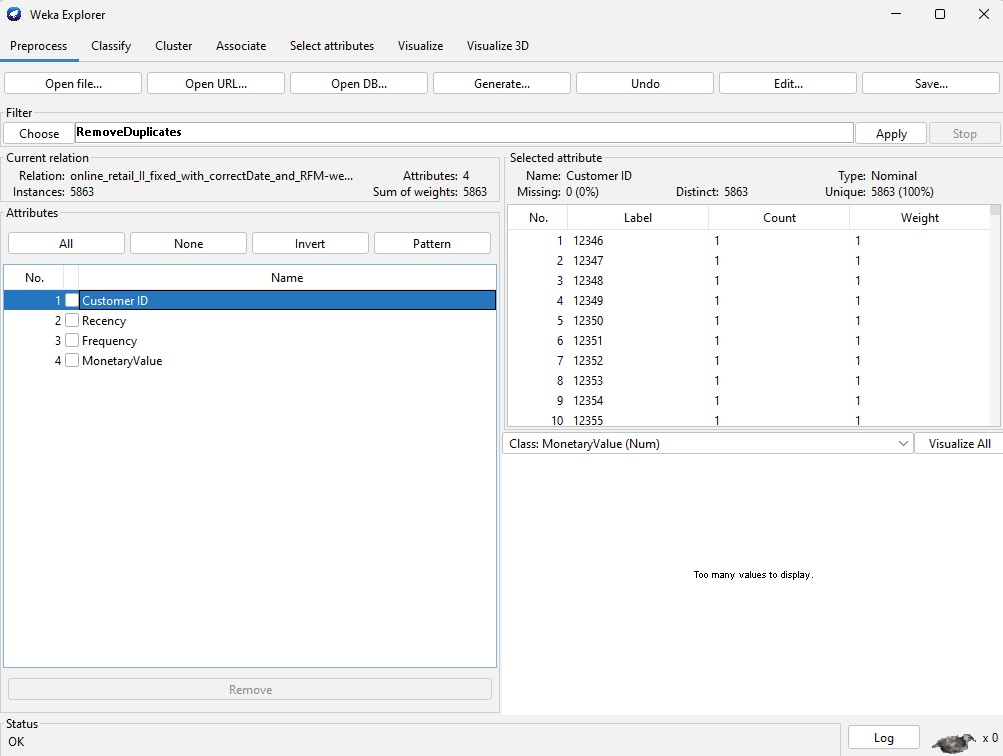
\includegraphics[width=1\linewidth]{imagens/figure5.jpg}\label{cap-2-fig5}
    \captionof{figure}[LOF entry]{Resultado final após aplicação do filtro \textit{\textbf{RemoveDuplicates}}.}
    \label{fig5}
    \end{centering}
\end{figure}

Como podemos verificar, a aplicação do filtro \textit{\textbf{RemoveDuplicates}} permitiu-nos reduzir a dimensão do nosso conjunto de dados de 793380 instâncias para apenas 5863. Cada uma das instâncias que permanece diz respeito apenas a um cliente. Caso não se efetuasse a remoção de instâncias duplicadas, ao se aplicar os algoritmos de classificação, estes seriam sobreajustados, pois cada cliente teria multiplas linhas associadas, o que causaria um sobreajuste nas nossas métricas de desempenho.
Agora que os nossos dados estão preparados, iremos passar à segmentação de clientes.

%----------------------------------------------------------------------------------------------------------


%----------------------------------------------------------------------------------------------------------
\section{Segmentação de Clientes}
\subsection{Escolha do número e tipo de \textit{bins}}

Antes de podermos realizar a segmentação de clientes, devemos normalizar os valores de RFM obtidos através da atribuição de pontuações (por exemplo, 1 sendo a pior, 10 sendo a melhor pontuação) para cada métrica. Como os valores de RFM podem variar muito para cada cliente, poderão não ser diretamente comparáveis. Ao atribuirmos pontuações, garantimos que clientes com comportamentos semelhantes sejam colocados no mesmo segmento. Outra vantagem é a mitigação de \textit{outliers}, pois poderão existir clientes com valores muito altos de Recência, Frequência e/ou valor Monetário que irão causar distorção nos nossos dados.
Para realizarmos a atribuição de pontuações, devemos discretizar os nossos dados em \textit{bins}. Para isso, podemos utilizar o \textit{software} \textit{\textbf{Weka}}, através do filtro \textit{\textbf{Discretize}}. No entanto, devemos olhar primeiro para os valores a discretizar, para verificarmos as distribuições dos seus valores e decidir se deveremos aplicar \textit{equal-frequency binning} ou \textit{equal-width binning}. Abaixo podemos encontrar gráficos que ilustram a distribuião dos nossos dados:

 \begin{figure}[H]
    \begin{centering}
    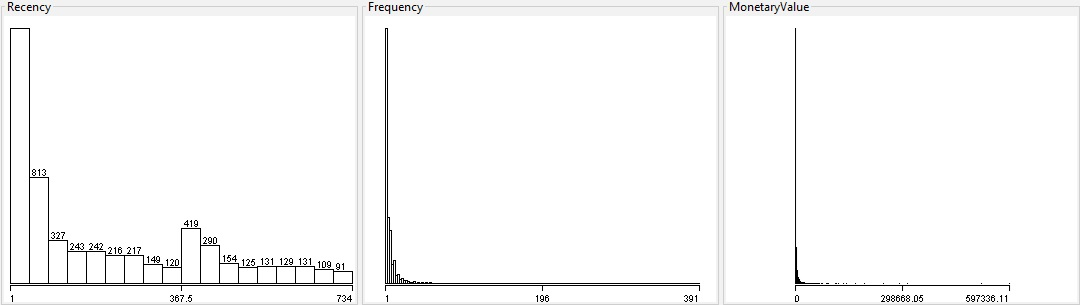
\includegraphics[width=1\linewidth]{imagens/figure6.jpg}\label{cap-3-fig6}
    \captionof{figure}[LOF entry]{Distribuições dos clientes por Recência, Frequência e valor Monetário.}
    \label{fig6}
    \end{centering}
\end{figure}

Como podemos verificar, existe uma grande discrepância nos valores de cada uma das métricas:

\begin{enumerate}
    \item \textbf{Recência}: Existe uma grande diferença entre os valores, com grande parte dos clientes tendo um valor de recência baixo, ou seja, esses clientes realizaram compras recentemente.
    \item \textbf{Frequência}: Existe uma grande diferença entre os valores, com grande parte dos clientes tendo um valor de Frequência baixo, ou seja, esses clientes realizaram compras pouco frequentemente.
    \item \textbf{Valor Monetário}: Existe uma grande diferença entre os valores, grande parte dos clientes  realizou compras cujo valor total é baixo, existem também outros clientes com valores monetários muito altos, provavelmente atacadistas (clientes que compram em grandes quantidades, possivelmente para revenda).
\end{enumerate}

Para podermos colmatar este problema, é recomendada a utilização de \textbf{\textit{equal-frequency binning}} \cite{RFMSDM2004}. Como os nossos dados não estão uniformemente distribuidos, a utilização desse tipo de separação irá permitir que cada \textit{bin} tenha aproximadamente o mesmo número de clientes,o que irá permitir balancear os segmentos de utilizador e permitir uma comparabilidade melhorada em todas as métricas.
O próximo passo é a decisão do número de \textit{bins}. Em teoria, quanto maior for o número de bins, melhor será a granularidade da nossa análise em segmentar os clientes, mas esse aumento da granularidade irá diminuir a nossa capacidade de interpretar os resultados finais e segmentar os clientes de acordo com a sua pontuação. Por exemplo, com a divisão em \textit{bins} de tamanho 10, se fossemos a mostrar os segmentos de clientes num gráfico 2D (Recência \textit{vs.} Frequência), teriamos uma grelha de tamanho 100 (10x10). O problema torna-se mais complexo se adicionarmos uma terceira dimensão (valor monetário), teriamos 1000 (10x10x10) zonas diferentes no gráfico de segmentos de clientes. 
Para efeitos da análise realizada ao conjunto de dados neste documento, iremos então escolher um número de \textit{bins} mais modesto, com a discretização a ser efetuada com 5 \textit{bins}. Com esta separação, o gráfico 2D da nossa análise, quando compararmos Recência \textit{vs.} Frequência, terá 25 zonas (5x5), o gráfico 3d será composto por 125 zonas (5x5x5).

\newpage
\subsection{Discretização e atribuição de pontuações RFM}

Antes de aplicarmos a discretização dos nossos atributos, devemos criar uma cópia dos mesmos por forma a não se perder os valores originais de RFM. Para isso, devemos utilizar o filtro \textit{\textbf{AddExpression}} da seguinte forma, para cada um dos atributos:

 \begin{figure}[H]
    \begin{centering}
    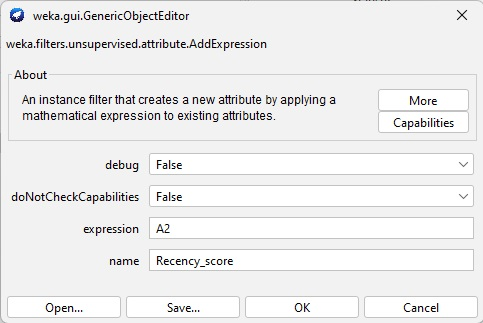
\includegraphics[width=0.5\linewidth]{imagens/figure12.jpg}\label{cap-3-fig12}
    \captionof{figure}[LOF entry]{Aplicação do filtro \textit{\textbf{AddExpression}} para o atributo \textit{Recency}.}
    \label{fig12}
    \end{centering}
\end{figure}

 \begin{figure}[H]
    \begin{centering}
    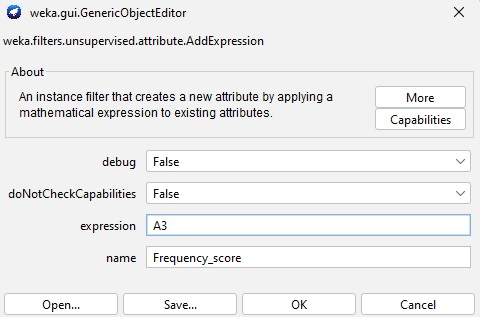
\includegraphics[width=0.5\linewidth]{imagens/figure13.jpg}\label{cap-3-fig13}
    \captionof{figure}[LOF entry]{Aplicação do filtro \textit{\textbf{AddExpression}} para o atributo \textit{Frequency}.}
    \label{fig13}
    \end{centering}
\end{figure}

 \begin{figure}[H]
    \begin{centering}
    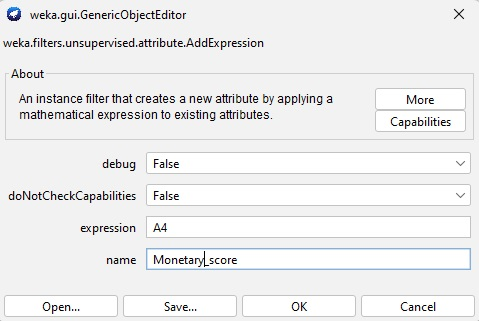
\includegraphics[width=0.5\linewidth]{imagens/figure14.jpg}\label{cap-3-fig14}
    \captionof{figure}[LOF entry]{Aplicação do filtro \textit{\textbf{AddExpression}} para o atributo \textit{Monetary Value}.}
    \label{fig14}
    \end{centering}
\end{figure}

Após a criação das cópias dos nossos atributos RFM, iremos aplicar a discretização aos mesmos. Anteriormente, ficou decidida a utilização de \textit{\textbf{equal-frequency binning}} com 5 \textit{bins}. Para podermos realizar essa operação, iremos utilizar o \textit{Weka}, mais específicamete o seu fitro \textit{\textbf{Discretize}}. A figura \ref{fig7} demonstra a aplicação do filtro, bem como os parâmetros a ser definidos:

 \begin{figure}[H]
    \begin{centering}
    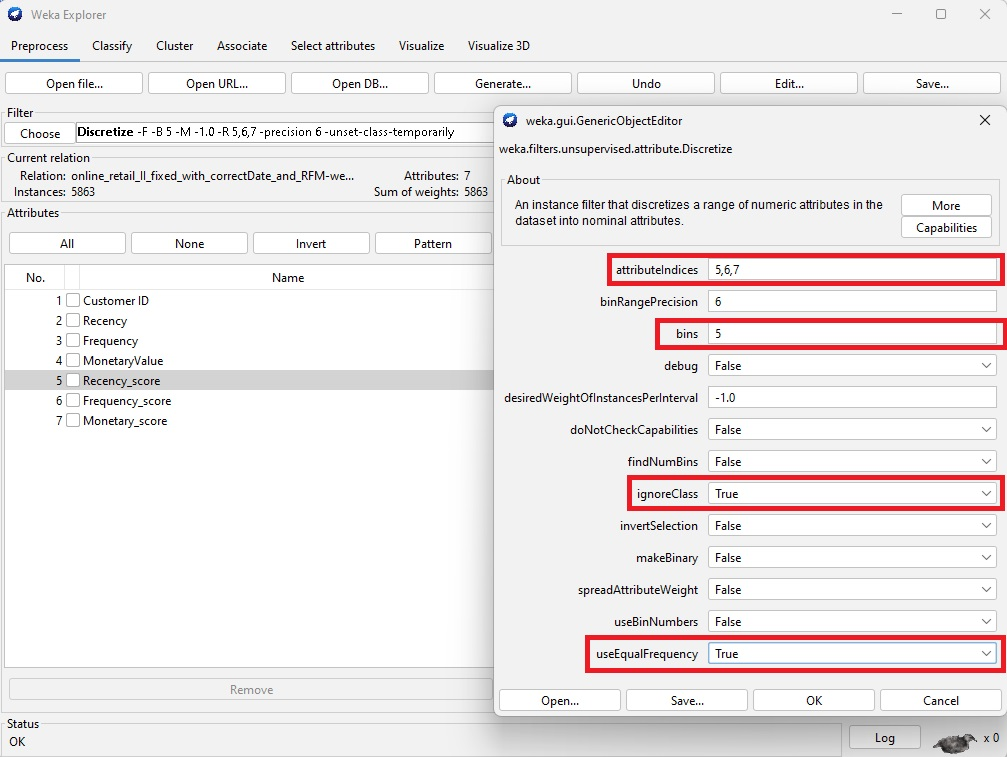
\includegraphics[width=1\linewidth]{imagens/figure7.jpg}\label{cap-4-fig7}
    \captionof{figure}[LOF entry]{Distribuições dos clientes por Recência, Frequência e valor Monetário.}
    \label{fig7}
    \end{centering}
\end{figure}

\begin{enumerate}
    \item \textbf{\textit{atributesIndices}}: Nesta opção, indicamos quais os índices dos atributos aos quais queremos aplicar a discretização. Devemos colocar "5,6,7" (sem as aspas).
    \item \textbf{\textit{bins}}: Nesta opção, é feita a definição do número de \textit{bins}. Para efeitos deste artigo, iremos utilizar 5 \textit{bins}.
    \item \textbf{\textit{ignoreClass}}: Nesta opção, indicamos que queremos ignorar o atributo classe. Escolhemos \textit{"True"}.
    \item \textbf{\textit{useEqualFrequency}}: Nesta opção, indicamos que queremos realizar o \textit{binning} com \textit{equal-frequency binning}.
\end{enumerate}

\newpage

Depois de aplicarmos a discretização, os valores de Recência, Frequência e Valor Monetário serão agrupados em 5 \textit{bins} de acordo com a sua frequência. A figura \ref{fig8} mostra o resultado final da discretização:

\begin{figure}[H]
    \begin{centering}
    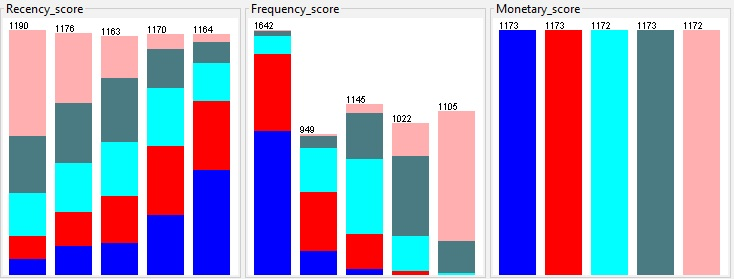
\includegraphics[width=1\linewidth]{imagens/figure8.jpg}\label{cap-4-fig8}
    \captionof{figure}[LOF entry]{Distribuições dos clientes por Recência, Frequência e valor Monetário, por 5 \textit{bins}.}
    \label{fig8}
    \end{centering}
\end{figure}

Como podemos verificar, a utilização de \textit{\textbf{equal-frequency binning}} permitiu-nos balancear os dados, criando células com o número aproximado de clientes. Apenas no caso da Frequência é que houve um menor balanceamento, mas isso poderá ser explicado pela grande diferença entre os hábitos de compras dos clientes, com grande prevalência de clientes com poucas compras realizadas.

O próximo passo é o renomear dos \textit{bins} obtidos para valores numéricos de 1 a 5, em que valores mais altos indicam pontuação mais elevada:

\begin{enumerate}
	\item[\textbullet] \textbf{Recência}: Quanto menor a recência, melhor a pontuação.
	\item[\textbullet] \textbf{Frequência}: Quanto maior a frequência, melhor a pontuação.
	\item[\textbullet] \textbf{Valor Monetário}: Quanto maior o valor monetário, melhor a pontuação.
\end{enumerate}

Para realizarmos a operação de renomear os diferentes \textit{bins} iremos utilizar o filtro \textit{\textbf{RenameNominalValues}}. Este filtro permite indicar os valores a substituir e o seu substituto, podendo realizar multiplas substituições de uma vez só. Para cada um dos atributos RFM, iremos realizar as seguintes substituições:

\begin{enumerate}
	\item \textbf{Recência}:
		\item[\textbullet] \textbf{(-inf-19.5]}: 5
		\item[\textbullet] \textbf{(19.5-59.5]}: 4
		\item[\textbullet] \textbf{(59.5-193.5]}: 3
		\item[\textbullet] \textbf{(193.5-406.5]}: 2
		\item[\textbullet] \textbf{(406.5-inf)}: 1

\newpage

	\item \textbf{Frequência}:
		\item[\textbullet] \textbf{(-inf-1.5]}: 1
		\item[\textbullet] \textbf{(1.5-2.5]}: 2
		\item[\textbullet] \textbf{(2.5-4.5]}: 3
		\item[\textbullet] \textbf{(4.5-8.5]}: 4
		\item[\textbullet] \textbf{(8.5-inf)}: 5
	\item \textbf{Valor Monetário}:
		\item[\textbullet] \textbf{(-inf-285.67]}: 1
		\item[\textbullet] \textbf{(285.67-612.69]}: 2
		\item[\textbullet] \textbf{(612.69-1231.44]}: 3
		\item[\textbullet] \textbf{(1231.44-2932.06]}: 4
		\item[\textbullet] \textbf{(2932.06-inf)}: 5
\end{enumerate}


Abaixo podemos encontrar a aplicação do filtro para todos os atributos RFM:

\begin{figure}[H]
    \begin{centering}
    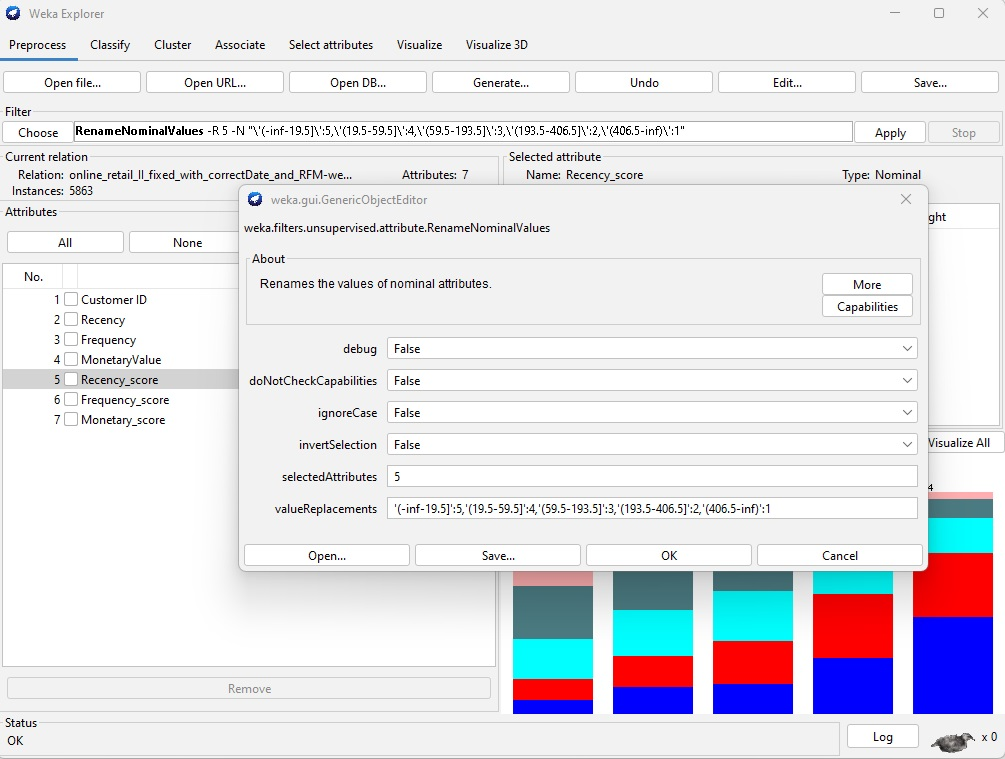
\includegraphics[width=0.85\linewidth]{imagens/figure9.jpg}\label{cap-4-fig9}
    \captionof{figure}[LOF entry]{Alteração do nome dos intervalos de Recência para refletir a pontuação.}
    \label{fig9}
    \end{centering}
\end{figure}

\begin{figure}[H]
    \begin{centering}
    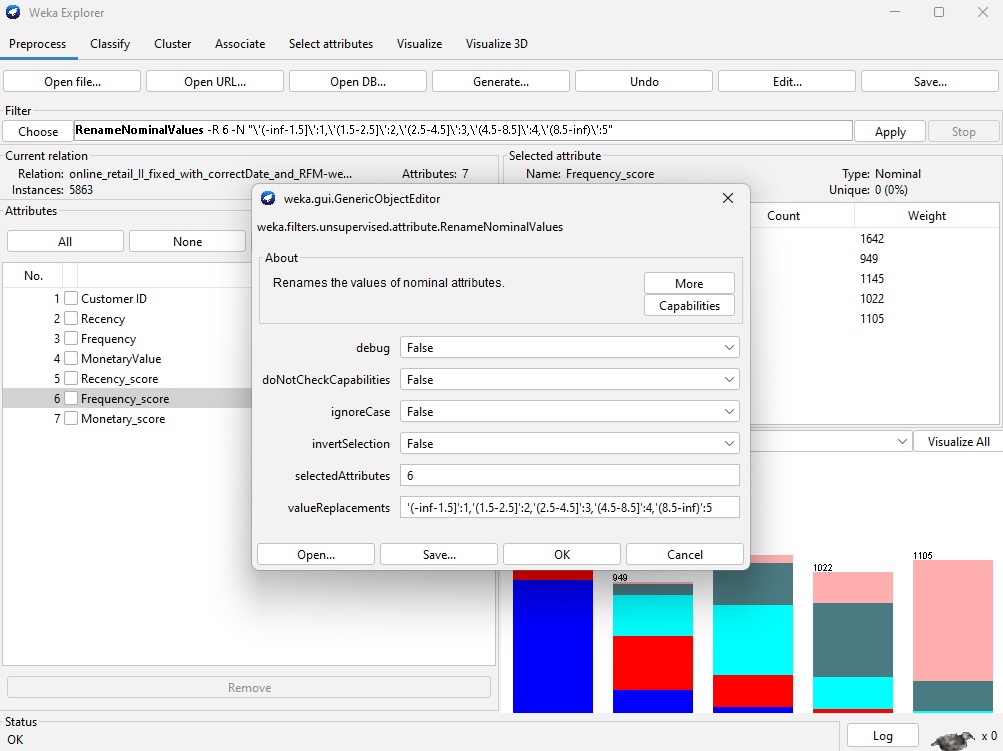
\includegraphics[width=0.85\linewidth]{imagens/figure10.jpg}\label{cap-4-fig10}
    \captionof{figure}[LOF entry]{Alteração do nome dos intervalos de Frequência para refletir a pontuação.}
    \label{fig10}
    \end{centering}
\end{figure}

\begin{figure}[H]
    \begin{centering}
    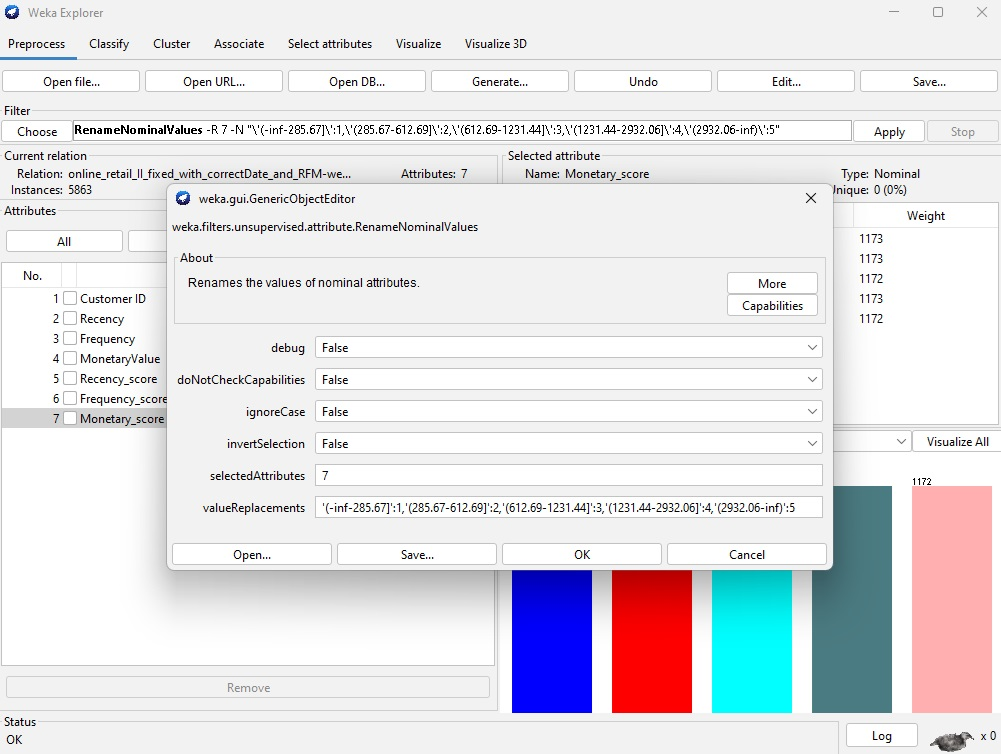
\includegraphics[width=0.85\linewidth]{imagens/figure11.jpg}\label{cap-4-fig11}
    \captionof{figure}[LOF entry]{Alteração do nome dos intervalos do valor Monetário para refletir a pontuação.}
    \label{fig11}
    \end{centering}
\end{figure}

O próximo passo é a segmentação dos clientes de acordo com os valores de pontuação RFM. Para isso, devemos converter primeiro os atributos de pontuação de nominal para numéricos. Uma forma simples de o fazer sem recorrer a nenhum filtro no \textit{Weka} é guardar o trabalho realizado até aqui como um ficheiro .arff, abrir o ficheiro num editor de texto e alterar o tipo de dados no cabeçalho para os atributos \textit{\textbf{Recency_score}}, \textit{\textbf{Frequency_score}} e \textit{\textbf{Monetary_score}} de \textit{\textbf{nominal}} (removendo a lista de atributos nominais) para \textit{\textbf{numeric}}.

\begin{figure}[H]
    \begin{centering}
    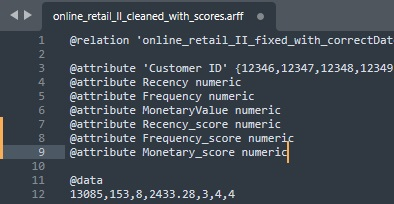
\includegraphics[width=0.8\linewidth]{imagens/figure15.jpg}\label{cap-4-fig15}
    \captionof{figure}[LOF entry]{Alteração do tipo de dados das pontuações RFM de nominal para numérico com o editor \textit{\textbf{Sublime Text}}.}
    \label{fig15}
    \end{centering}
\end{figure}

Quando voltarmos a abrir o \textit{Weka}, os nossos atributos já serão interpretados como atributos numéricos. De seguida, iremos proceder à segmentação dos clientes com base nos valores de pontuação RFM, utilizando para esse efeito o \textit{\textbf{K-means Clustering}}. No entanto, será necessário escolher o número de segmentos de cliente com base nas pontuações. Para esse efeito, iremos utilizar o chamado \textit{\textbf{Elbow Method}}\cite{RCCAFRM}.
O \textit{\textbf{Elbow Method}} ajuda-nos a identificar o \textit{tradeoff} ótimo entre a complexidade do modelo e a variância explicada (a similaridade intra-\textit{cluster}). Além disso, a utilização de demasiados \textit{clusters} pode causar o sobreajustamento dos nossos dados (o chamado \textit{overfit}), em que são criados \textit{clusters} pequenos que não têm capacidade de generalização.
Testando multiplos valores de K na aba \textit{\textbf{Cluster}} no \textit{Weka}, obtemos o seguinte resultado:

\begin{table}[htb]
\centering
\begin{tabular}{l|l|l|l}
Número de Clusters & Within Cluster Sum of Squared Errors  & Diferença &   \\
\hline
2                  & 989.8093476                                    &         &   \\
3                  & 755.0489622                                    & -23.7177\%  &   \\
4                  & 540.0345318                                    & -28.4769\% &   \\
5                  & 457.3705245                                    & -15.3072\%  &   \\
6                  & 407.868599                                     & -10.8232\%  &   \\
7                  & 369.9222038                                    & -9.30358\%  &   \\
8                  & 348.0911701                                    & -5.90152\%  &   \\
9                  & 321.9408009                                    & -7.51251\%  &   \\
10                 & 285.7621183                                    & -11.2377\%  &  
\end{tabular}
\end{table}

\begin{figure}[H]
    \begin{centering}
    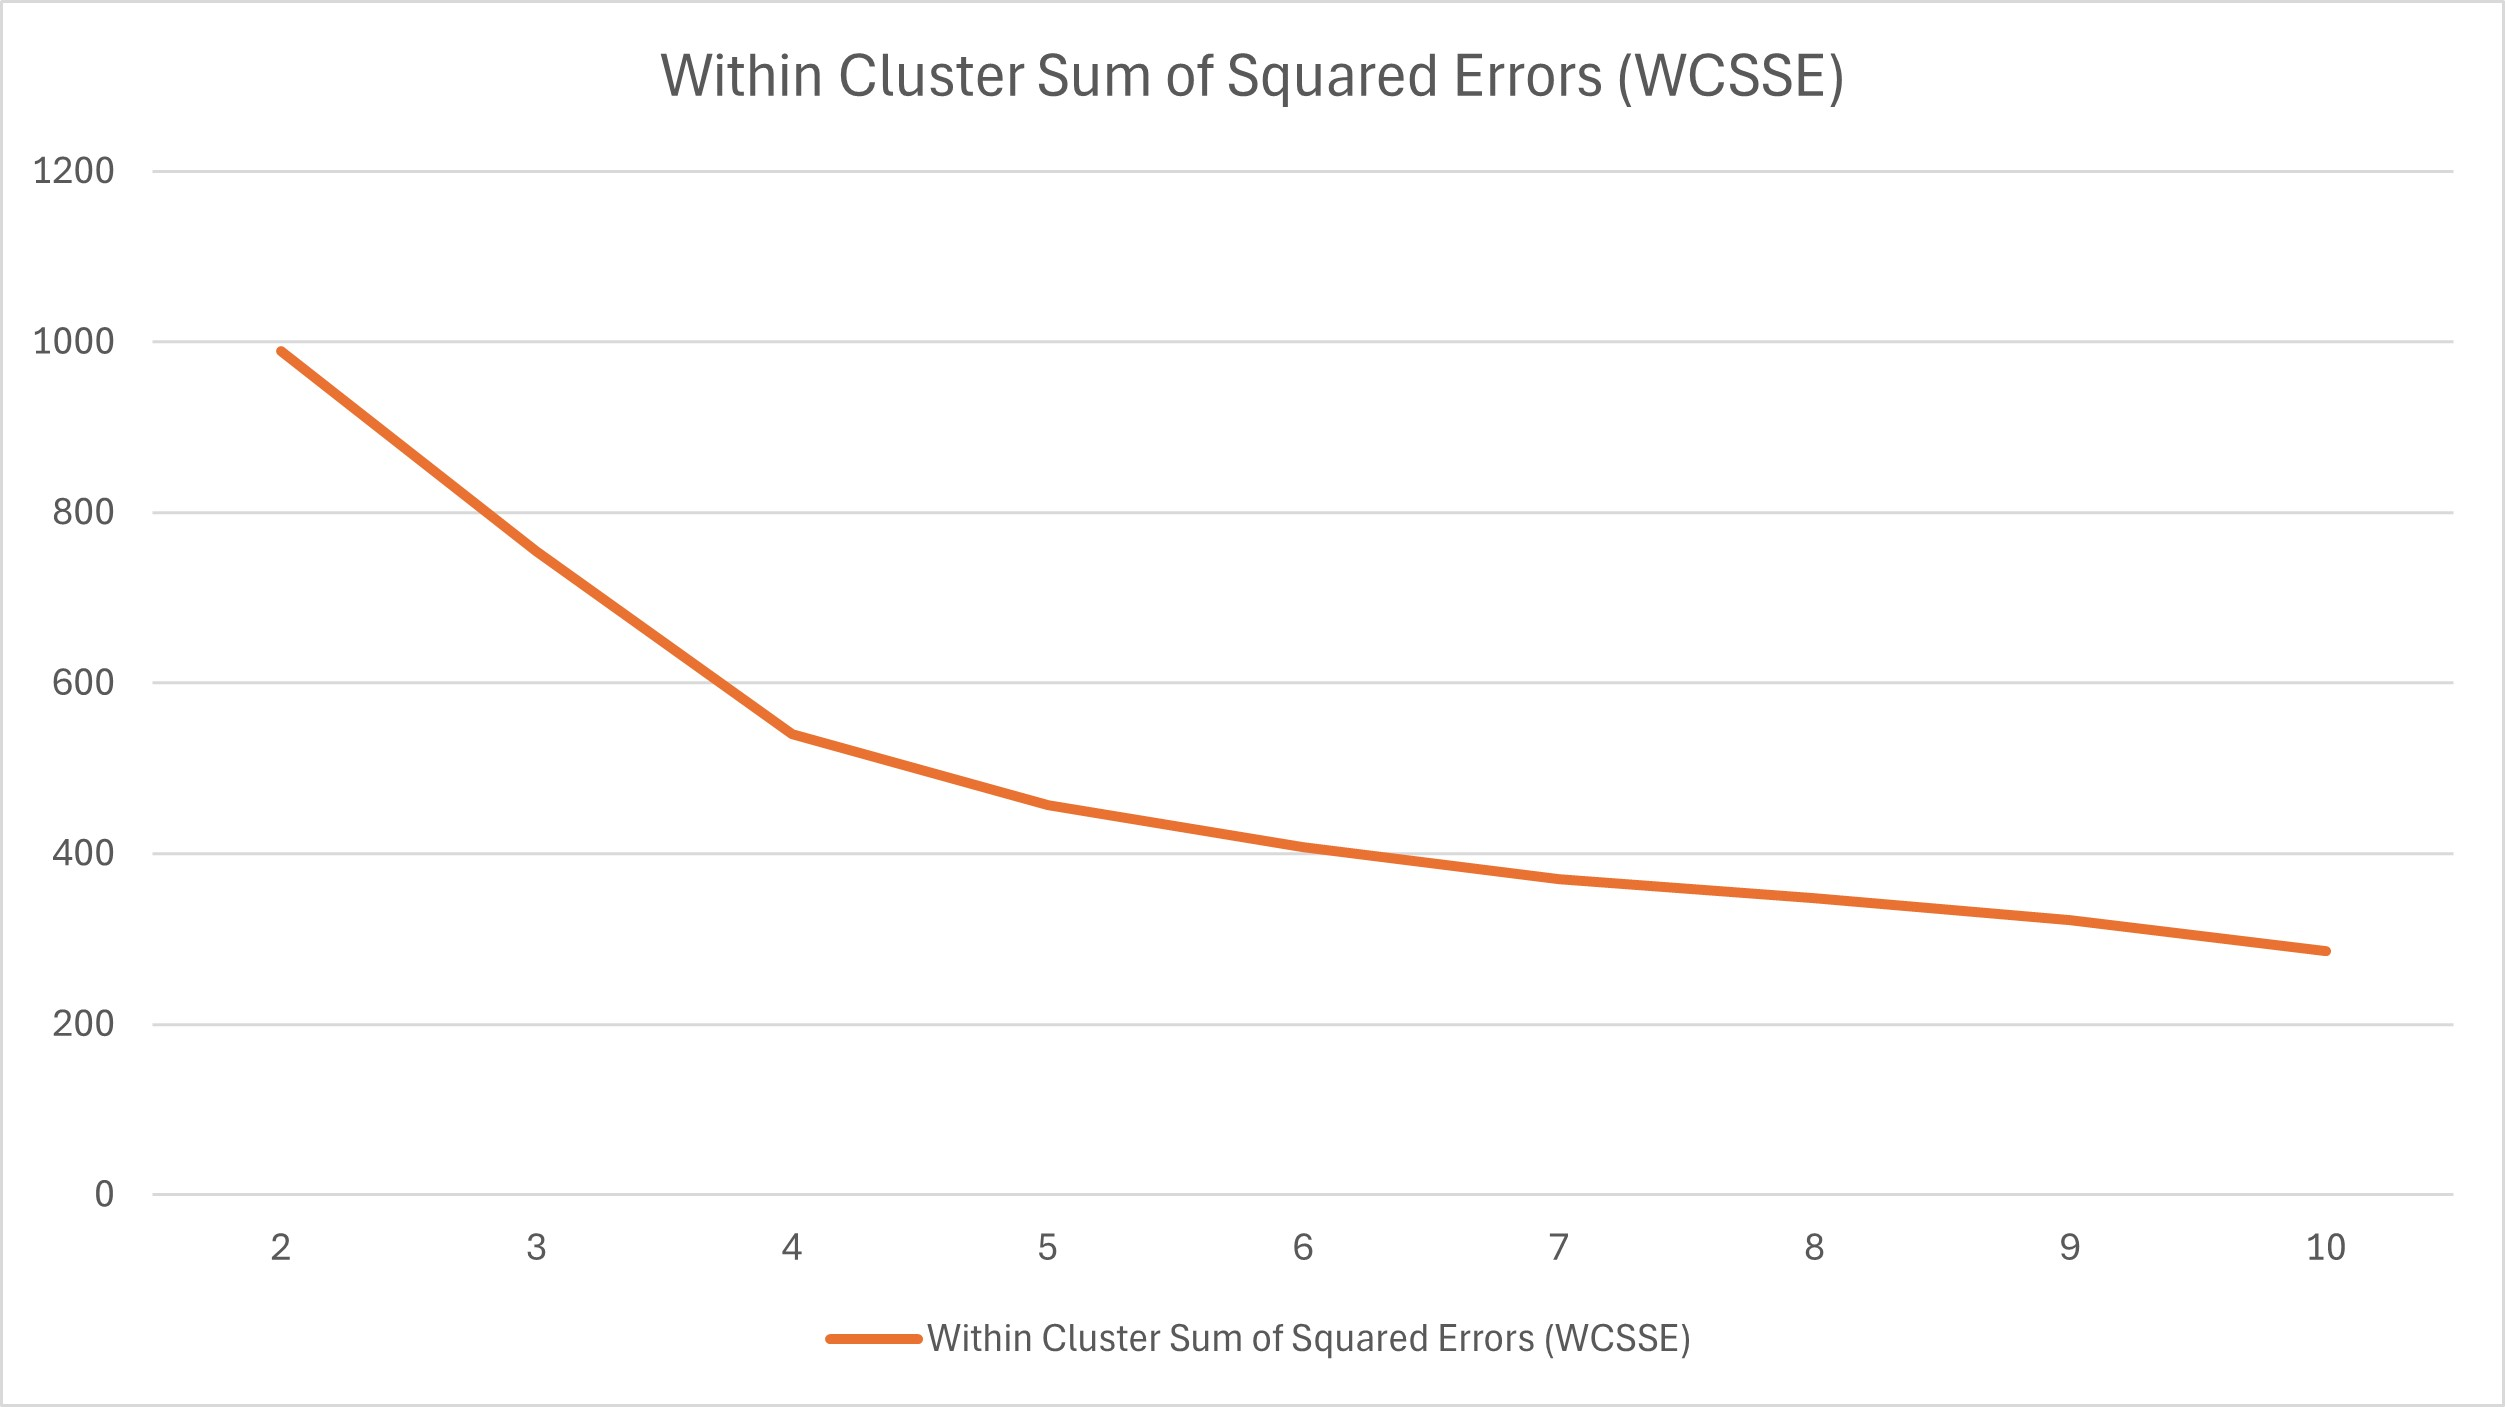
\includegraphics[width=1\linewidth]{imagens/figure16.jpg}\label{cap-4-fig16}
    \captionof{figure}[LOF entry]{Curva que ilustra a redução cada vez mais expressiva nos valores de erro.}
    \label{fig16}
    \end{centering}
\end{figure}


Com base nos resultados anteriores, iremos escolher o valor de 5 para o número de \textit{clusters}, dado que valores superiores de K oferecem um ganho cada vez mais diminuto.
A segmentação de clientes pode ser definida então como uma questão de troca (\textit{tradeoff}) ou balanceamento entre a granularidade da análise e a sua complexidade. Com a utillização de 5 \textit{clusters}, a nossa segmentação de clientes irá ter em conta apenas 5 grupos distintos de clientes:

\begin{enumerate}
    \item \textbf{Clientes VIP}: Estes são os melhores clientes, que compram frequentemente, gastam muito e realizaram compras recentemente.
		\item[\textbullet] \textbf{Recência}: Muito recente.
		\item[\textbullet] \textbf{Frequência}: Muito frequente.
		\item[\textbullet] \textbf{Valor Monetário}: Muito alto.
    \item \textbf{Clientes Fiéis}: Estes clientes compram regularmente, mas gastam de forma moderada.
		\item[\textbullet] \textbf{Recência}: Recente.
		\item[\textbullet] \textbf{Frequência}: Muito frequente.
		\item[\textbullet] \textbf{Valor Monetário}: Moderado.
    \item \textbf{Grandes Gastadores Ocasionais}: Estes clientes gastam muito quando compram, mas fazem-no raramente.
		\item[\textbullet] \textbf{Recência}: Moderado.
		\item[\textbullet] \textbf{Frequência}: Pouco Frequente.
		\item[\textbullet] \textbf{Valor Monetário}: Muito alto.
    \item \textbf{Clientes em Risco}: Estes clientes compram com pouca frequência e gastam pouco quando o fazem.
		\item[\textbullet] \textbf{Recência}: Recente a moderado.
		\item[\textbullet] \textbf{Frequência}: Pouco Frequente.
		\item[\textbullet] \textbf{Valor Monetário}: Baixo.
    \item \textbf{Clientes Perdidos}: Não compram a muito tempo, gastaram pouco e compraram raramente.
		\item[\textbullet] \textbf{Recência}: Muito Antigo.
		\item[\textbullet] \textbf{Frequência}: Infrequente.
		\item[\textbullet] \textbf{Valor Monetário}: Muito Baixo.
\end{enumerate}


Agora que escolhemos o número de clusters, iremos voltar ao \textit{Weka} e iremos seleccionar o filtro \textit{\textbf{AddCluster}}. Na opção \textit{\textbf{ignoreAttributeIndices}}, escolhemos ignorar todos os atributos que não sejam as pontuações RFM, conforme a imagem abaixo:

\begin{figure}[H]
    \begin{centering}
    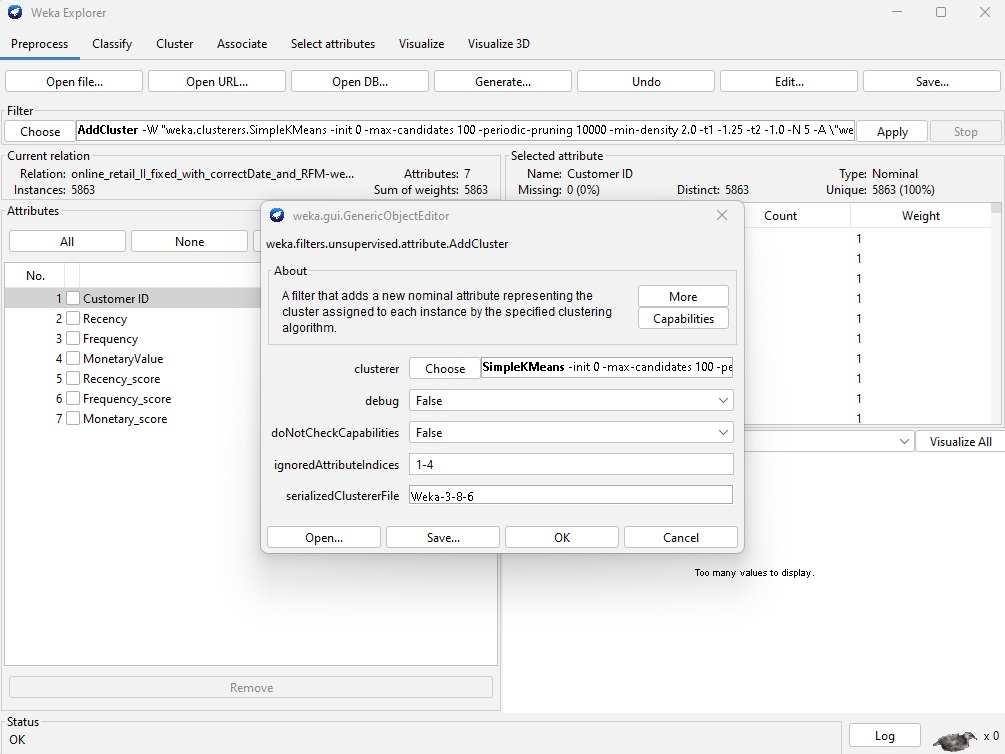
\includegraphics[width=1\linewidth]{imagens/figure17.jpg}\label{cap-4-fig17}
    \captionof{figure}[LOF entry]{Opções do filtro \textit{\textbf{AddCluster}}.}
    \label{fig17}
    \end{centering}
\end{figure}

De seguida, abrimos as opções do algoritmo de \textit{Clustering} e escolhemos na opção \textit{numClusters}, colocando o valor 5:

\begin{figure}[H]
    \begin{centering}
    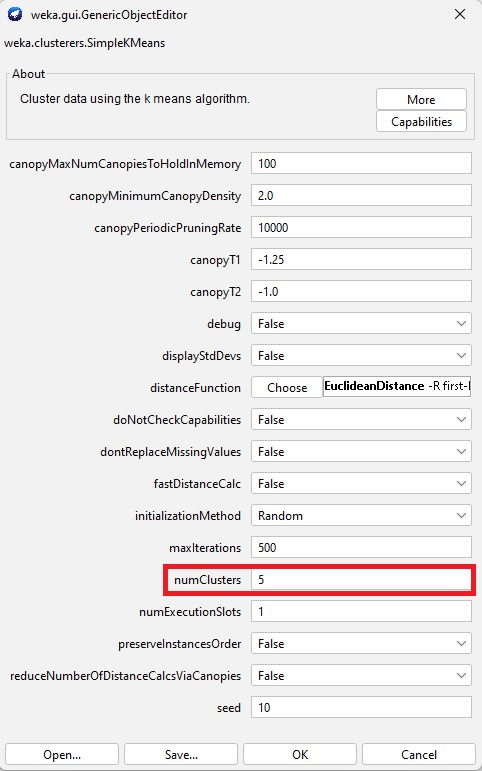
\includegraphics[width=0.4\linewidth]{imagens/figure18.jpg}\label{cap-4-fig18}
    \captionof{figure}[LOF entry]{Opções do filtro \textit{\textbf{AddCluster}}.}
    \label{fig18}
    \end{centering}
\end{figure}

Depois de aplicarmos o \textit{clustering} ao nosso conjunto de dados, obtemos a seguinte distribuição de instâncias por cada um dos \textit{clusters} (mais tarde iremos renomear cada um para que os nomes coincidam com os grupos definidos acima, mas primeiro precisamos de identificar cada um dos grupos):


\begin{figure}[H]
    \begin{centering}
    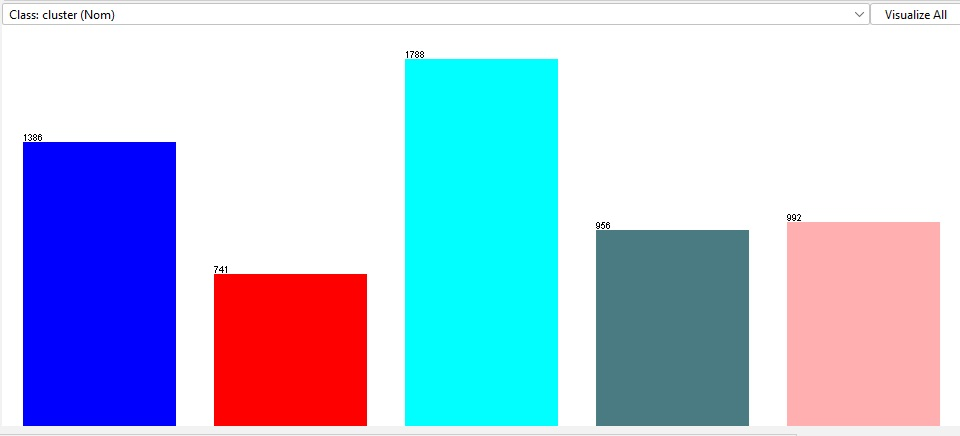
\includegraphics[width=1\linewidth]{imagens/figure19.jpg}\label{cap-4-fig19}
    \captionof{figure}[LOF entry]{Distribuição de instâncias por cada \textit{cluster}.}
    \label{fig19}
    \end{centering}
\end{figure}

\subsection{Cálculo do Risco de Abandono}

Outra métrica muito importante na análise RFM é o chamado risco de abandono de clientes (em inglês, \textit{\textbf{customer churn}}). Esta métrica indica a probabilidade que cada cliente tem, com base no seu histórico anterior, de vir a abandonar o negócio do qual o conjunto de dados diz respeito num futuro próximo.
Com base na informação do \textit{\textbf{churn}}, as empresas poderão definir estratégias para reter os clientes em risco.
Para calcular um valor normalizado na escala de [0...1] do risco de \textit{churn} para cada cliente, podemos utilizar a seguinte formula:

\[ \textit{ChurnRisk} = w_R*(1-\frac{RecencyScore}{Max(RecencyScore)}) + w_F*(1-\frac{FrequencyScore}{Max(FrequencyScore)}) + w_M*(1-\frac{MonetaryScore}{Max(MonetaryScore)})\]


Em que:

\begin{enumerate}
	\item[\textbullet] \textit{\textbf{ChurnRisk}}: Corresponde ao valor de risco de abandono normalizado, entre [0...1].
	\item[\textbullet] \textit{\textbf{wR}}: Corresponde a um valor de peso a atribuir à pontuação normalizada referente à recência, na escala de [0...1].
	\item[\textbullet] \textit{\textbf{wF}}: Corresponde a um valor de peso a atribuir à pontuação normalizada referente à frequência, na escala de [0...1].
	\item[\textbullet] \textit{\textbf{wM}}: Corresponde a um valor de peso a atribuir à pontuação normalizada referente ao valor monetário, na escala de [0...1].
	\item[\textbullet] \textit{\textbf{RecencyScore}}: Corresponde ao valor de pontuação atribuido à recência de determinado cliente, na escala de [1...5].
	\item[\textbullet] \textit{\textbf{FrequencyScore}}: Corresponde ao valor de pontuação atribuido à frequência de determinado cliente, na escala de [1...5].
	\item[\textbullet] \textit{\textbf{MonetaryScore}}: Corresponde ao valor de pontuação atribuido ao valor monetário de determinado cliente, na escala de [1...5].
	\item[\textbullet] \textit{\textbf{Max(.......)}}: Corresponde ao valor máximo de pontuação relativo a cada uma das componentes RFM. No caso deste conjunto de dados, o valor é sempre 5.
\end{enumerate}

\textit{\textbf{\underline{Nota}}}: A soma dos pesos wR, wF e wM deve de ser igual a 1, caso contrário arriscamos a subajustar ou sobreajustar o nosso modelo. A escolha de qual valor de pesos a aplicar irá depender da estratégia empresarial de cada organização, caso queiram dar mais enfâse à recência, frequência ou valor monetário das compras dos seus clientes. Para continuar o teste ao conjunto de dados deste artigo, iremos definir wR = 0.5, wF = 0.3 e wM = 0.2.
Para aplicarmos a fórmula acima a cada instância dos nossos dados, iremos utilizar novamente o filtro \textit{\textbf{AddExpression}}, criando um novo atributo chamado \textit{\textbf{ChurnRisk}}:

\begin{figure}[H]
    \begin{centering}
    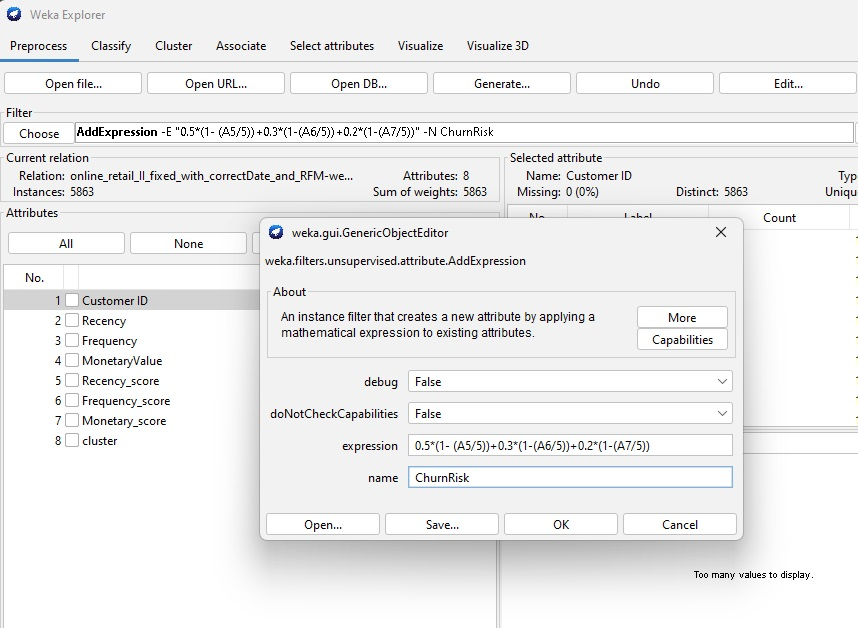
\includegraphics[width=1\linewidth]{imagens/figure20.jpg}\label{cap-4-fig20}
    \captionof{figure}[LOF entry]{Criação do novo atributo \textit{\textbf{ChurnRisk}}.}
    \label{fig20}
    \end{centering}
\end{figure}

Após aplicarmos o filtro, cada uma das instâncias terá um novo atributo numérico na escala de [0...1] que indica a probabilidade do cliente abandonar o negócio. O próximo passo será definir intervalos e um novo atributo nominal que indique qual o nível de risco (Baixo Risco, Alto Risco, ...). Para isso, voltamos a utilizar o filtro \textit{\textbf{AddExpression}} com a seguinte expressão:

\begin{figure}[H]
    \begin{centering}
    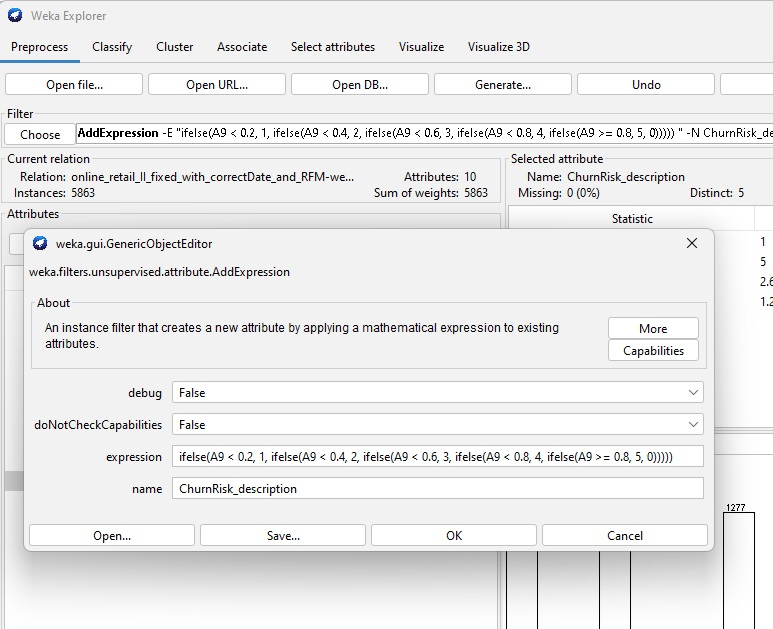
\includegraphics[width=1\linewidth]{imagens/figure21.jpg}\label{cap-4-fig21}
    \captionof{figure}[LOF entry]{Definição de intervalos de risco por cliente.}
    \label{fig21}
    \end{centering}
\end{figure}

De momento, este filtro criou um novo atributo numérico com valores entre 1 e 5, que indicam o nível de risco. No entanto, para ser mais legível, iremos converter o atributo de numérico para nominal e substituir os números por descrições mais facilmente interpretáveis. Para tal, iremos aplicar o filtro \textit{\textbf{NumericToNominal}}, escolhendo o atributo \textit{last}:

\begin{figure}[H]
    \begin{centering}
    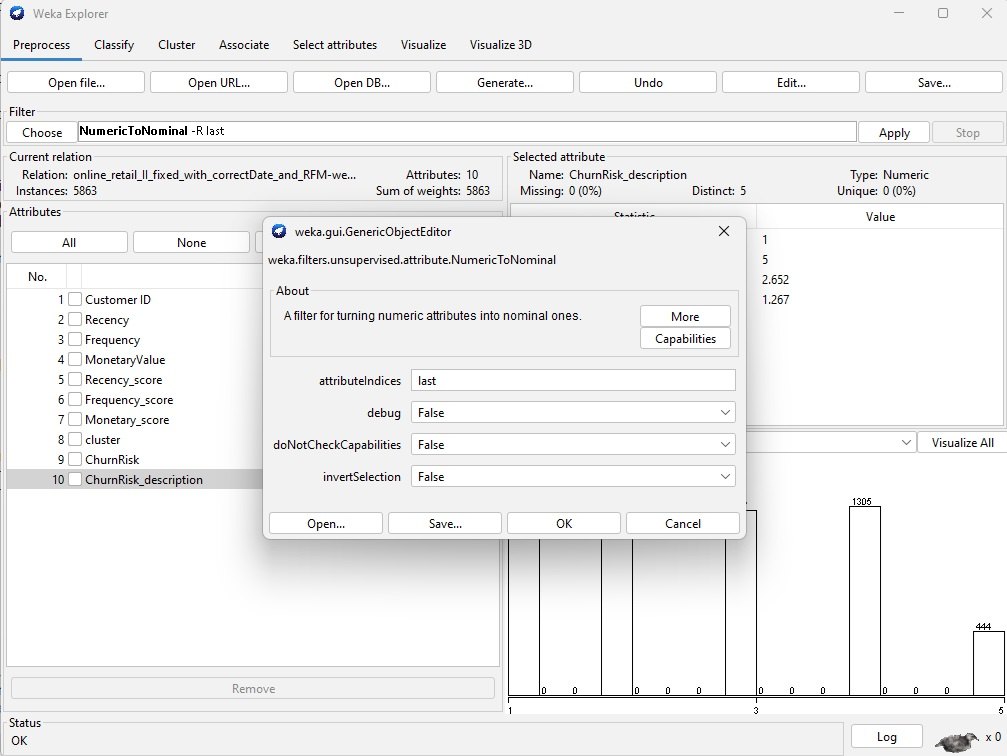
\includegraphics[width=1\linewidth]{imagens/figure22.jpg}\label{cap-4-fig22}
    \captionof{figure}[LOF entry]{Conversão do atributo \textit{\textbf{ChurnRisk_description}} de numérico para nominal.}
    \label{fig22}
    \end{centering}
\end{figure}

O último passo é a renomeação dos diferentes valores nominais de [1...5] numa descrição mais interpretável. Para isso, será necessário voltar a aplicar o filtro \textit{\textbf{RenameNominalValues}}, definindo as seguintes descrições por cada nível:

\begin{enumerate}
	\item[\textbullet] \textbf{1}: Muito Baixo Risco.
	\item[\textbullet] \textbf{2}: Baixo Risco.
	\item[\textbullet] \textbf{3}: Médio Risco.
	\item[\textbullet] \textbf{4}: Alto Risco.
	\item[\textbullet] \textbf{5}: Muito Alto Risco.
\end{enumerate}

\newpage
A figura seguinte ilustra a aplicação do nosso filtro de acordo com as regras acima:

\begin{figure}[H]
    \begin{centering}
    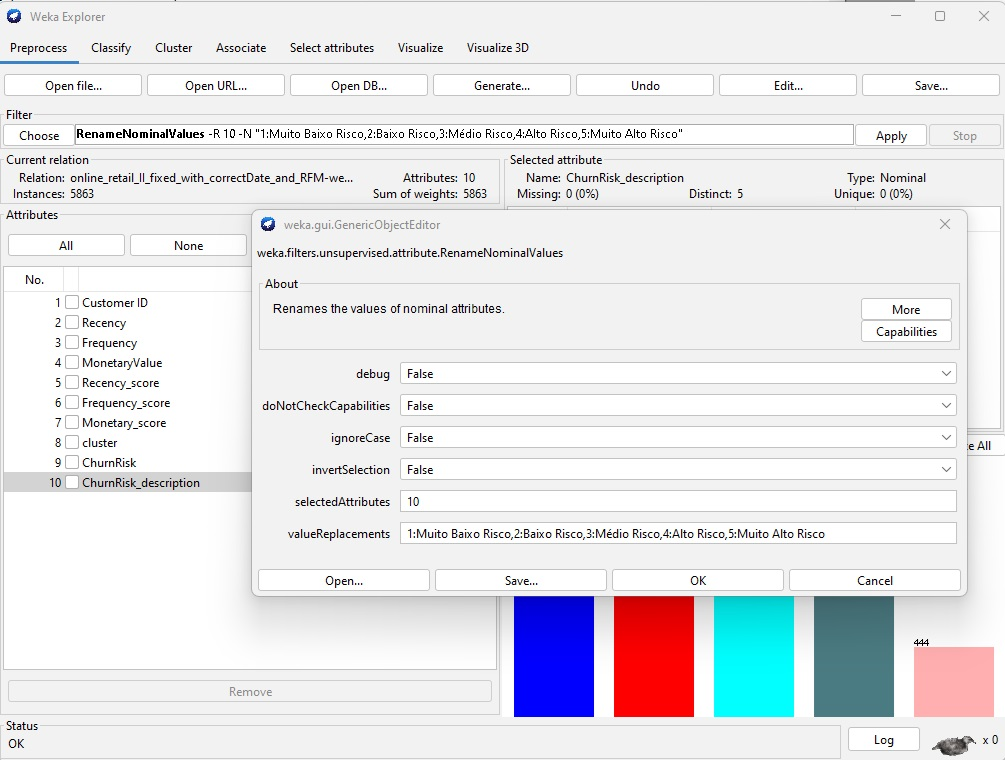
\includegraphics[width=1\linewidth]{imagens/figure23.jpg}\label{cap-4-fig23}
    \captionof{figure}[LOF entry]{Renomeação dos atributos nominais.}
    \label{fig23}
    \end{centering}
\end{figure}

\newpage

\section{Resultados}
\subsection{Visualização dos segmentos de clientes}

Depois de realizada a segmentação de clientes e o cálculo do risco de abandono, obtemos a seguinte distribuição dos segmentos de clientes:

\begin{figure}[H]
    \begin{centering}
    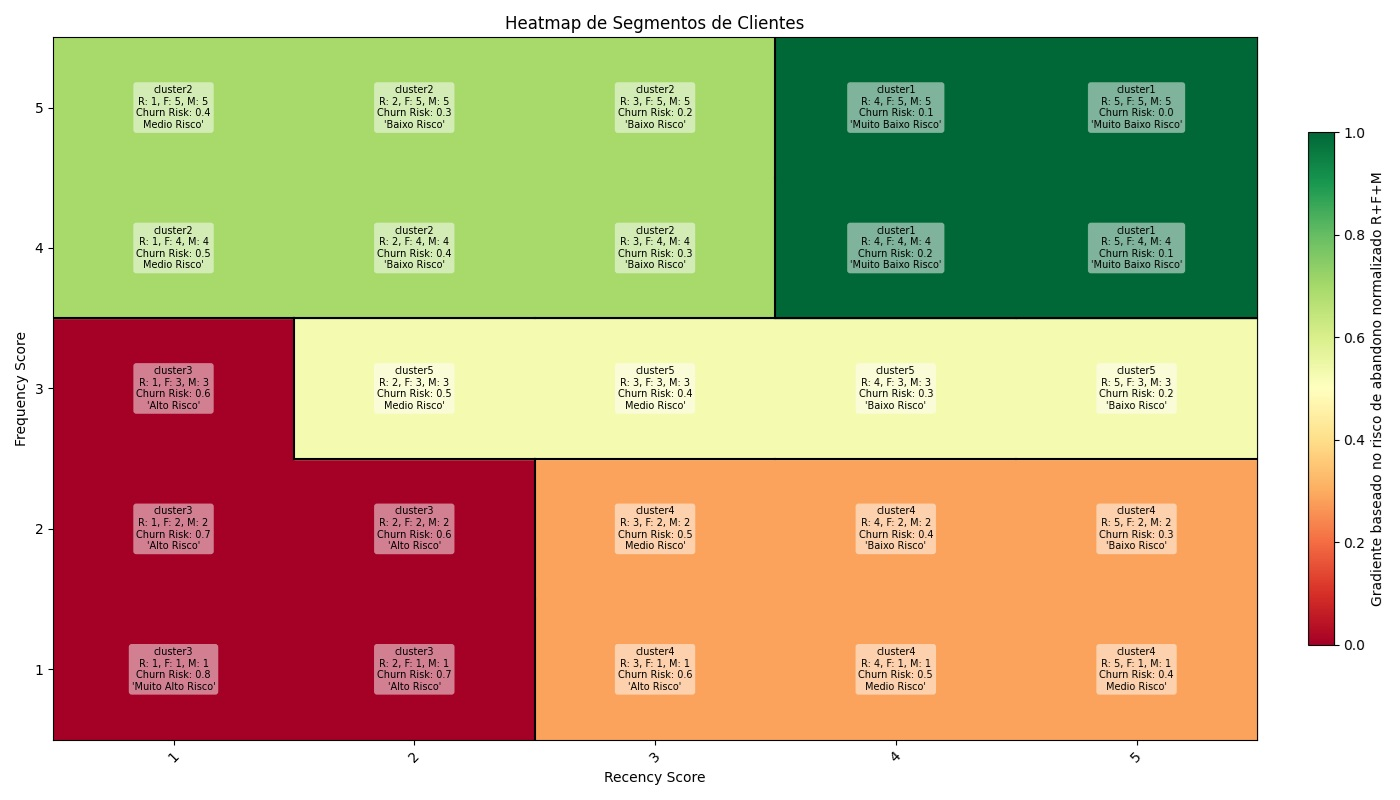
\includegraphics[width=0.8\linewidth]{imagens/figure24.jpg}\label{cap-5-fig24}
    \captionof{figure}[LOF entry]{Segmentos de Clientes, gráfico 2D \textit{Frequency_score vs. Recency_score}.}
    \label{fig24}
    \end{centering}
\end{figure}

Na figura \ref{fig24}, é feita uma comparação dos \textit{clusters} com base nos valores de pontuação da Recência e Frequência. Podemos verificar o seguinte:

\begin{enumerate}
	\item \textit{\textbf{Pontuações mais elevadas (Canto Superior Direito, Zonas Verdes)}}: Os clientes com valores de pontuação altos de \textbf{Recência} e \textbf{Frequência} representam clientes ativos. Têm os valores de risco de abandono mais baixos e representam os clientes mais leais.
	\item \textit{\textbf{Pontuações mais baixas (Canto Inferior Esquerdo, Zonas Vermelhas)}}: Os clientes com valores de pontuação baixos de \textbf{Recência} e \textbf{Frequência} representam clientes inativos. Têm os valores de risco de abandono mais elevados e representam os clientes que deverão necessitar de estratégias de reativação.
	\item \textit{\textbf{Pontuações intermédias (Centro, Zonas Amarelas)}}: São clientes com valores pontuação de \textbf{Frequência} e \textbf{Valor Monetário} médios, e com valores de pontuação de \textbf{Recência} entre o baixo e alto. Apresentam valores médios de risco de abandono [0.2 - 0.5] e necessitam de estratégias que permitam aumentar a interação (\textbf{Recência}) dos mesmos com a organização, para que possam mover para segmentos superiores e reduzir o risco de abandono.
	\item \textit{\textbf{Pontuações baixas (Canto Inferior Direito, Zonas Laranja)}}: São clientes com valores pontuação de \textbf{Frequência} e \textbf{Valor Monetário} muito baixos e com \textbf{Recência} média a alta. Têm risco de abandono moderado [0.3 - 0.6]. Podem estar aqui representados os clientes mais novos (aqueles com \textbf{Recência} alta e \textbf{Frequência} baixa), como tal, poderá ser importante a implementação de estratégias que permita aumentar a retenção desses clientes, fomentando a realização de novas compras e com valores superiores, além de contribuir para a diminuição do risco de abandono.
	\item \textit{\textbf{Pontuações altas (Canto Superior Esquerdo, Zonas Verde-Claro)}}: São clientes com valores de \textbf{Frequência} e \textbf{Valor Monetário} elevados mas com \textbf{Recência} moderada a baixa. Têm risco de abandono baixo a moderado [0.2 - 0.5]. Estes clientes necessitam da implementação de estratégias que permita aumentar a sua recência (por exemplo através de ofertas ou promoções).
\end{enumerate}

\begin{figure}[H]
    \begin{centering}
    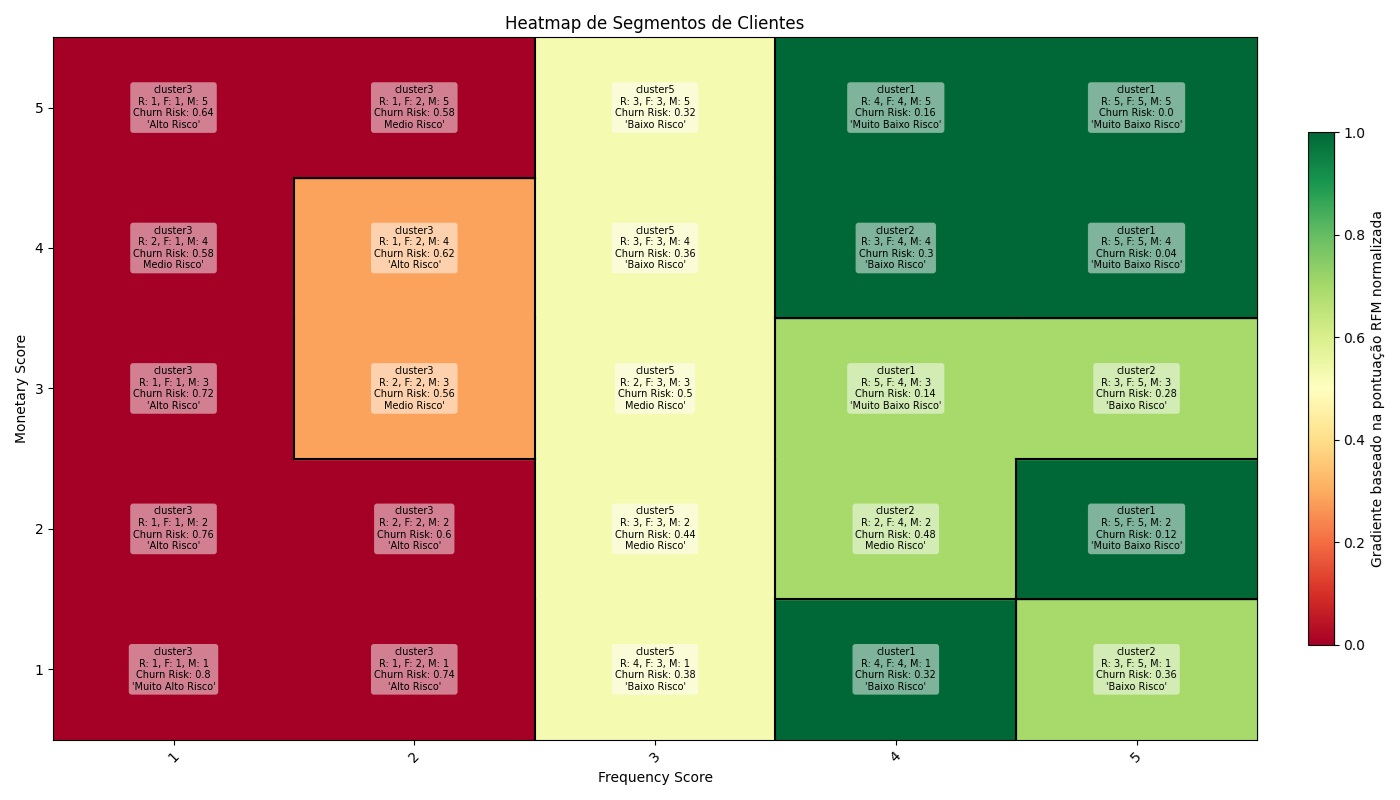
\includegraphics[width=0.8\linewidth]{imagens/figure27.jpg}\label{cap-5-fig27}
    \captionof{figure}[LOF entry]{Segmentos de Clientes, gráfico 2D \textit{Monetary_score vs. Frequency_score}.}
    \label{fig76}
    \end{centering}
\end{figure}

\begin{enumerate}
	\item \textit{\textbf{Pontuações mais elevadas (Topo Superior Direito, Zonas Verdes)}}: Os clientes com valores de pontuação altos de \textbf{Valor Monetário} e \textbf{Frequência} representam clientes ativos. Têm os valores de risco de abandono mais baixos e representam os clientes mais valiosos. A curto/médio prazo, não inspiram cuidados.
	\item \textit{\textbf{Pontuações mais baixas (Lado Esquerdo, Zonas Vermelhas)}}: Os clientes com valores de pontuação baixos de \textbf{Valor Monetário} e \textbf{Frequência} representam clientes inativos ou em alto risco de se tornarem inativos. Têm os valores de risco de abandono mais elevados [0.58 - 0.8] e representam os clientes que deverão necessitar de estratégias de reativação.
	\item \textit{\textbf{Pontuações Intermédias (Centro, Zonas Amarelas)}}: Os clientes com valores de pontuação intermédia de \textbf{Frequência} representam clientes que compram com alguma frequência e com valor monetário baixo a elevado mas com recência baixa a moderada. São bons candidados para a realização de estratégias que possibilitem o aumento do seu valor monetário. Os seus valores de risco de abandono são médios a moderados [0.32 - 0.5], o que é necessário monitorizar por forma a que não se tornem clientes inativos.
	\item \textit{\textbf{Pontuações elevadas (Lado Direito, Zonas Verde-Claro)}}: Os clientes nas zonas verde-claro compram com alguma frequência mas com valores de pontuação monetária mais baixa. Poderão ser alvos de estratégias de negócio que os posicionem em segmentos de clientes mais elevados desde que se cativem a comprar produtos de valor mais elevado. Têm um risco de abandono de baixo a moderado [0.14 - 0.48], os clientes com valores mais baixos não inspiram cuidados, poderá ser necessário monitorizar os clientes que apresentem risco mais elevado.
	\item \textit{\textbf{Pontuações baixas (Lado Esquerdo, Zonas Laranja)}}: Os clientes nas zonas laranja apresentam valores de \textbf{Recência} e \textbf{Frequência} mais baixos, com valores monetários moderados. Estes clientes deverão ser alvo de estratégias que aumentem a frequência de compras, como a utilização de cupões de desconto para permitir aumentar a recência e a frequência de compras. Estes clientes apresentam valores elevados de risco de abandono [0.56 - 0.62] e à semelhança dos clientes nas zonas vermelhas, necessitam de estratégias que permita aumentar a interação dos mesmos com a organização.
\end{enumerate}

\begin{figure}[H]
    \begin{centering}
    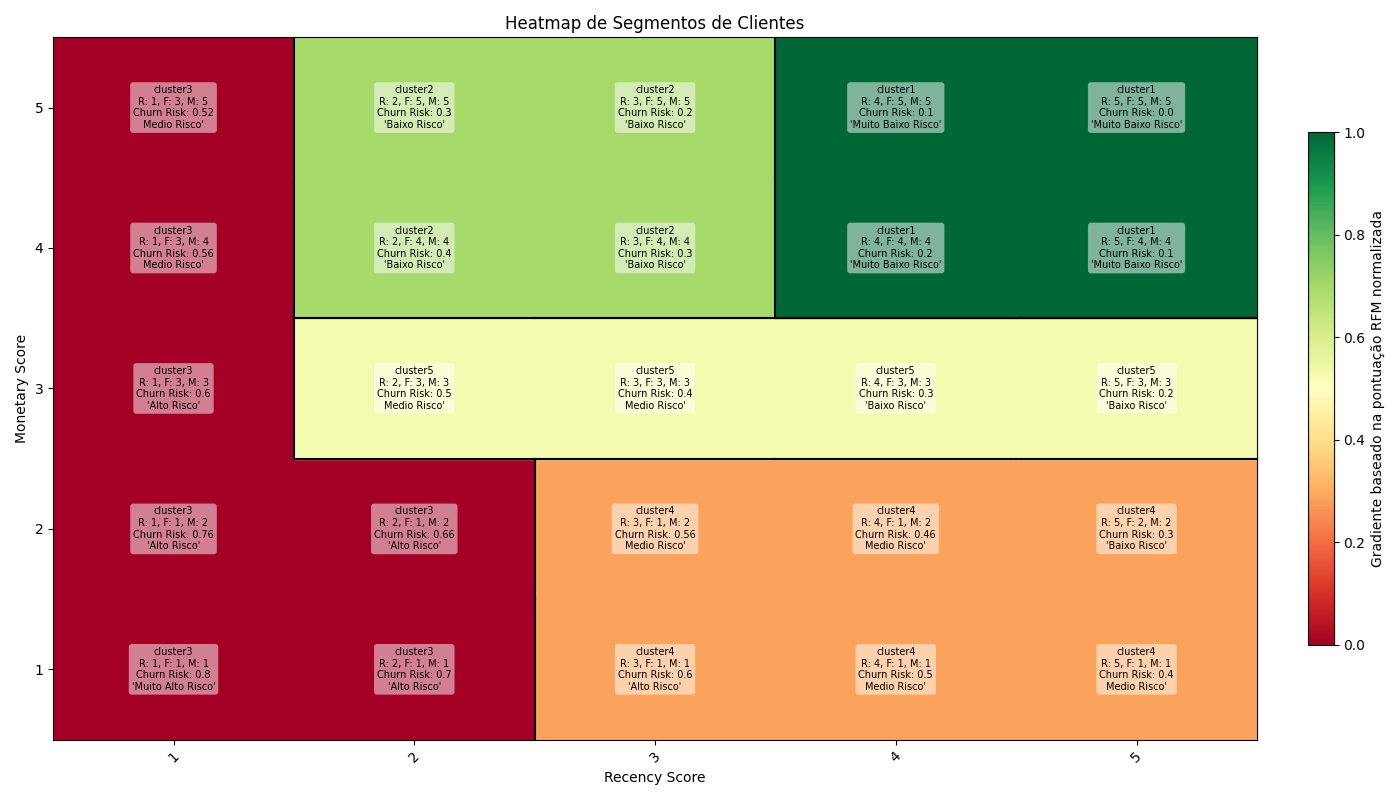
\includegraphics[width=0.8\linewidth]{imagens/figure28.jpg}\label{cap-5-fig28}
    \captionof{figure}[LOF entry]{Segmentos de Clientes, gráfico 2D \textit{Monetary_score vs. Recency_score}.}
    \label{fig28}
    \end{centering}
\end{figure}

Através da leitura do gráfico 2D, podemos interpretar os diferentes \textit{clusters} obtidos e interpretar quais os segmentos a que podem ser mapeados. Com base no gráfico, podemos referir:

\begin{enumerate}
	\item \textit{\textbf{Pontuações mais baixas (Lado Esquerdo, Zonas Vermelhas)}}: Os clientes nas zonas vermelhas são clientes inativos que apresentam valores de \textbf{Recência} extremamente baixos, indicando que não realizam compras à muito tempo. Em termos de \textbf{Frequência} têm valores que vão do baixo ao moderado, o que indica que realizaram poucas compras. A pontuação atribuida ao \textbf{Valor Monetário} indica que estes clientes realizaram compras de valor muito baixo até valores muito elevados. O seu risco de abandono é muito elevado [0.52 - 0.8]. Estes clientes necessitam de estratégias empresariais muito agressivas para aliciar estes clientes a voltarem ao ativo, com foco no aumento da pontuação de recência e na frequência de compras.
	\item \textit{\textbf{Pontuações mais elevadas (Canto Superior Direito, Zonas Verde Escuro)}}: Os clientes nas zonas verde escuro são os melhores clientes, com valores de pontuação de \textbf{Recência}, \textbf{Frequência} e \textbf{Valor Monetário} extremamente elevados. Também apresentam valores de risco de abandono extremamente baixos [0 - 0.2]. Não são clientes preocupantes a curto prazo.
	\item \textit{\textbf{Pontuações baixas (Canto Inferior Direito, Zonas Laranja)}}: Os clientes nas zonas laranja são clientes com valores de pontuação de \textbf{Recência} que vão do elevado ao moderado. As pontuações de \textbf{Frequência} e \textbf{Valor Monetário} são extremamente baixas. O seu risco de abandono é moderado [0.3 - 0.6]. Estes clientes realizaram um pequeno número de compras de valor baixo num passado relativamente recente. É necessário implementar estratégias que permitam aumentar a interação destes clientes com a organização com o objetivo de aumentar a pontuação de \textbf{Frequência} e \textbf{Valor Monetário} e permitir a subida de segmento destes clientes, ao mesmo tempo que se reduz o risco de abandono.
	\item \textit{\textbf{Pontuações intermédias (Centro, Zonas Amarelas)}}: Os clientes nas zonas amarelas são clientes com valores médios de \textbf{Recência}, \textbf{Frequência} e \textbf{Valor Monetário}. O seu risco de abandono vai do baixo ao moderado [0.2 - 0.5]. Estes clientes inspiram algum cuidado, pois as suas pontuações intermédias podem indicar flutuações crescentes ou decrescentes, podendo ficar em risco ou tornar-se bons clientes. É necessário acompanhar estes clientes e fomentar a sua interação com a organização para diminuir o seu risco de abandono ao mesmo tempo que se tenta aumentar as restantes métricas.
	\item \textit{\textbf{Pontuações altas (Centro Superior, Zonas Verde Claro)}}: Os clientes nas zonas verde-claro apresentam valores de \textbf{Frequência} e \textbf{Valor Monetário} altos, apenas tendo valores de \textbf{Recência} que médio-baixos. O seu risco de abandono é baixo [0.2 - 0.4]. Estes clientes embora apresentem risco de abandono baixo, irão beneficiar de estratégias que permitam aumentar a sua pontuação de recência. Estas estratégias irão permitir também reduzir ainda mais o risco de abandono.
\end{enumerate}


Visualizando cada \textbf{\textit{cluster}} num gráfico 3D:

\begin{figure}[H]
    \begin{centering}
    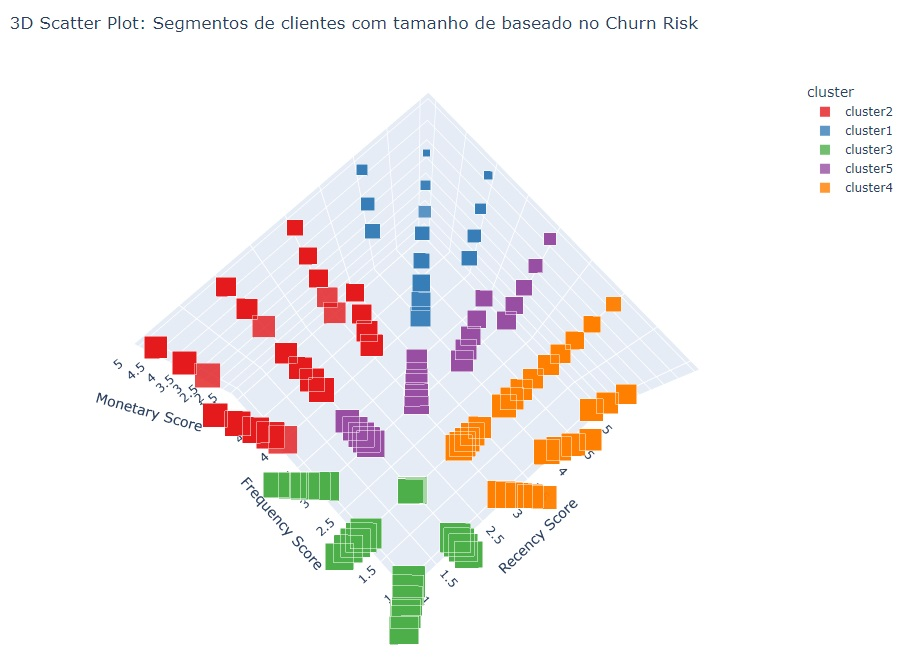
\includegraphics[width=1\linewidth]{imagens/figure25.jpg}\label{cap-5-fig25}
    \captionof{figure}[LOF entry]{Segmentos de Clientes, gráfico 3D \textit{Frequency_score vs. Recency_score vs. Monetary_score}.}
    \label{fig25}
    \end{centering}
\end{figure}

Através deste gráfico, podemos verificar que cada combinação de pontuações de \textbf{Recência}, \textbf{Frequência} e \textbf{Valor Monetário} pertence única e exclusivamente a um cluster, não havendo sobreposições (o que indica classes bem definidas e separadas). O tamanho de cada ponto depende do risco de abandono, com valores mais próximos de RFM:\{1,1,1\} a indicar maior risco e RFM:\{5,5,5\} a indicar menor risco.


\begin{figure}[H]
    \begin{centering}
    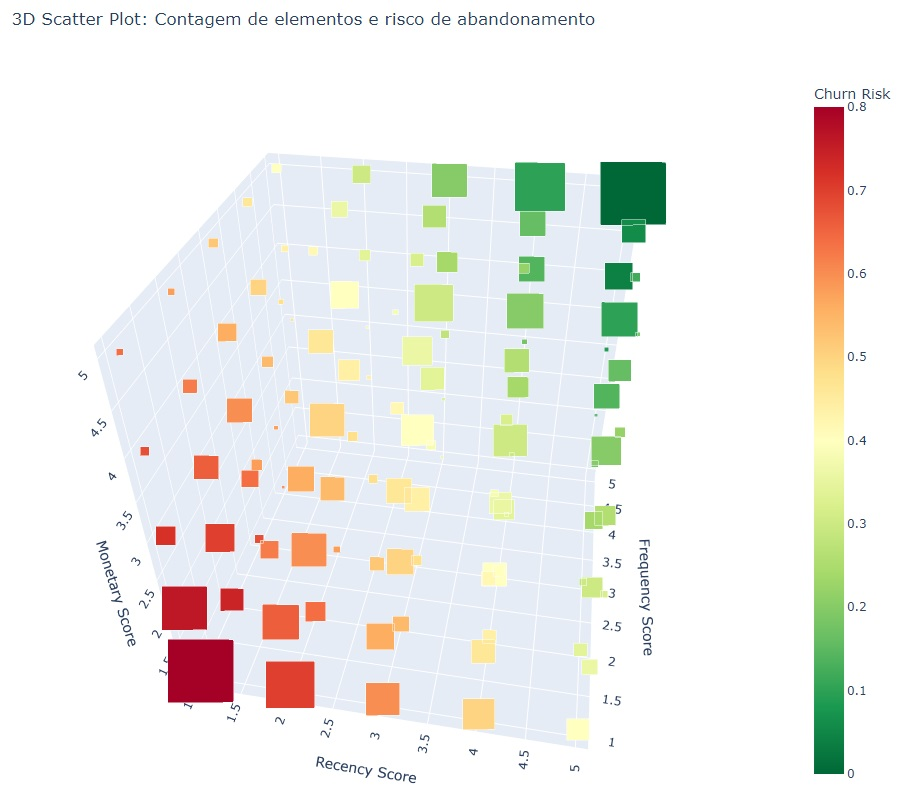
\includegraphics[width=1\linewidth]{imagens/figure31.jpg}\label{cap-5-fig31}
    \captionof{figure}[LOF entry]{Densidade de Clientes por Cluster (cor indica o risco de abandono), gráfico 3D \textit{Frequency_score vs. Recency_score vs. Monetary_score}.}
    \label{fig31}
    \end{centering}
\end{figure}

O gráfico acima indica que existe maior concentração de clientes nas zonas com RFM:\{1,1,1\} e RFM:\{5,5,5\}. Nas zonas onde o risco de abandono é maior (cor vermelha) será necessário a implementação de estratégias de retenção de clientes. A separação dos \textit{clusters} por pontuação de RFM no gráfico 3D permite vez quais as zonas de pontuação com maior densidade de clientes e quais as métricas que inspiram maiores cuidados. Desse modo, torna-se mais fácil visualizar quais os grupos que serão afetados pela implementação de estratégias específicas, além de se poder ver a evolução das concentrações de clientes ao longo do tempo, realizando-se multiplos \textit{plots} em diferentes momentos e comparando as distribuições.


\newpage
\subsection{Visualização do Risco de Abandono}

Visualizamos também o risco de abandono, comparado entre as diferentes métricas:

\begin{figure}[H]
    \begin{centering}
    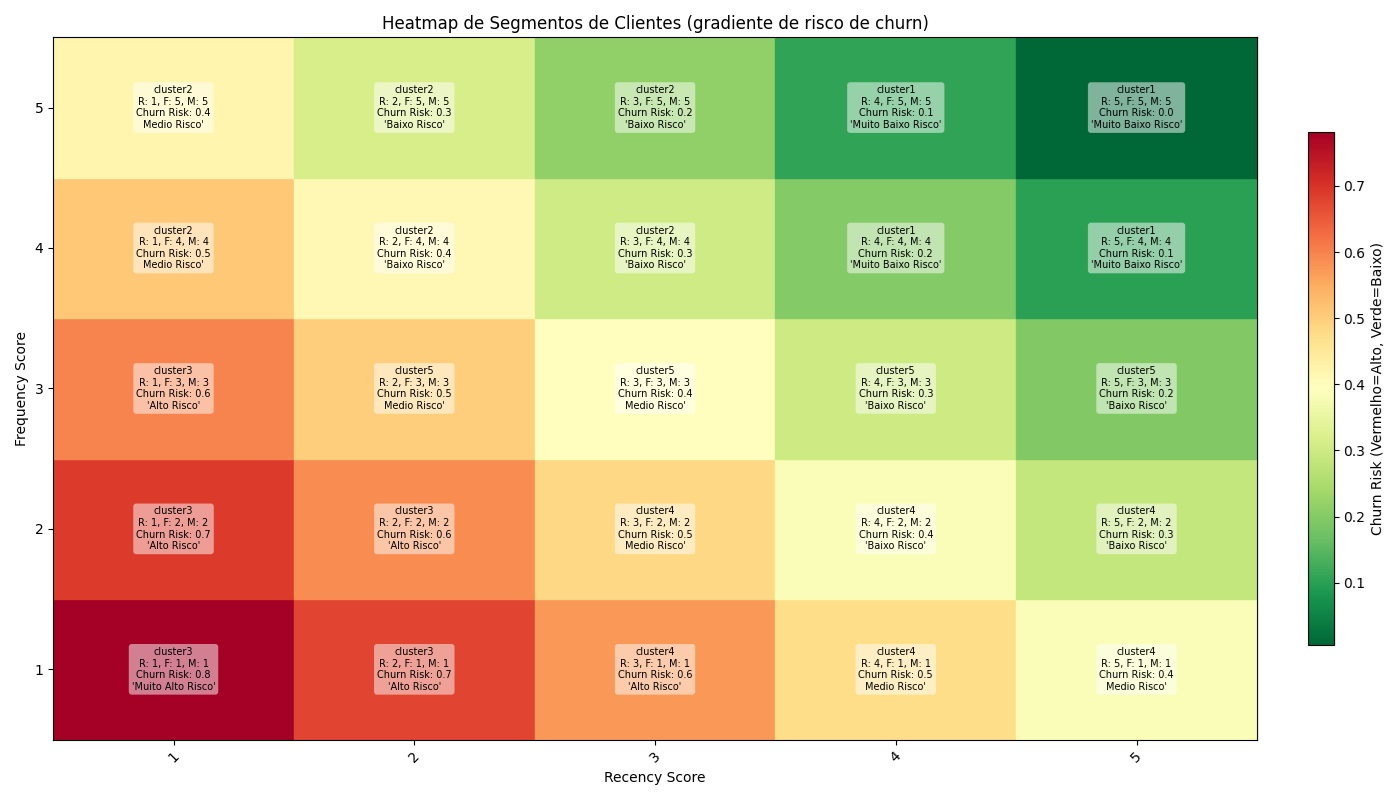
\includegraphics[width=1\linewidth]{imagens/figure26.jpg}\label{cap-5-fig26}
    \captionof{figure}[LOF entry]{Risco de \textbf{\textit{Churn}}, gráfico 2D \textit{Frequency_score vs. Recency_score}.}
    \label{fig26}
    \end{centering}
\end{figure}

\begin{enumerate}
	\item \textit{\textbf{Cores verdes (Risco mais baixo)}}: Os clientes nas zonas onde o risco é mais baixo [0.0 - 0.3] são clientes que compraram recentemente e realizam compras de forma frequente. Em termos de pontuação de \textbf{Valor Monetário} estes clientes gastaram valores baixos a elevados. Estes clientes devem ser mantidos através de programas de fidelização ou estratégias personalizadas.
	\item \textit{\textbf{Cor amarela (Risco médio-baixo)}}: Estes clientes apresentam o mesmo risco de abandono [0.4].

Por um lado, existem os clientes com alta pontuação de \textbf{Frequência} e \textbf{Valor Monetário}, mas baixa \textbf{Recência}. Estes clientes no passado compraram com frequência e com gastos elevados, mas por algum motivo deixaram de comprar à bastante tempo.

Por outro lado, existem clientes com alta pontuação de \textbf{Recência} e \textbf{Valor Monetário} mas baixa \textbf{Frequência}. Estes clientes compraram muito recentemente e com gastos elevados, mas por algum motivo realizaram poucas compras.

No centro do gráfico, temos os clientes com pontuações médias de \textbf{Recência}, \textbf{Frequência} e \textbf{Valor Monetário}. Estes clientes não compram a um período moderado de tempo, realizaram um número moderado de compras e essas compras tinham valores moderados.

Os clientes nas zonas amarelas apresentam comportamentos muito dispares entre si, necessitando de estratégias de negócio que sejam adequadas ao seu comportamento.
	\item \textit{\textbf{Cores laranja (Risco médio-alto)}}: Estes clientes apresentam risco médio-alto de abandono [0.5 - 0.6].

Nestes clientes, quanto maior a pontuação de \textbf{Recência}, menores as pontuações de \textbf{Frequência} e \textbf{Valor Monetário}, ou seja quanto mais recente a compra, menor o valor investido e o número de compras realizado. O que indica que por um lado temos clientes muito novos que depois não voltaram a repetir as compras, ou antigos clientes leais que por algum motivo deixaram de comprar. Deverão ser implementados estudos para verificar quais as causas que levaram ao \textit{disengagement} destes clientes, se foi falta de comunicação ou desinteresse nos produtos. Depois de realizado o estudo, deverão ser oferecidos incentivos para voltar a reaver esses clientes.
	\item \textit{\textbf{Cores vermelhas (Risco muito alto)}}: Estes clientes apresentam risco muito alto de abandono [0.7 - 1].

Estes clientes apresentam valores de pontuação muito baixos em todas as métricas, o que indica que foram clientes que compraram uma ou poucas vezes mas, por algum motivo não foram retidos. À semelhança dos clientes situados nas zonas laranja, estes deverão ser alvos de estudos que permitam perceber quais as razões da sua inatividade. Depois de apuradas as razões, deverão haver tentativas de os voltar a aproximar da organização, com por exemplo, oferta de descontos, programas de fidelização, brindes, entre outros.
\end{enumerate}


\begin{figure}[H]
    \begin{centering}
    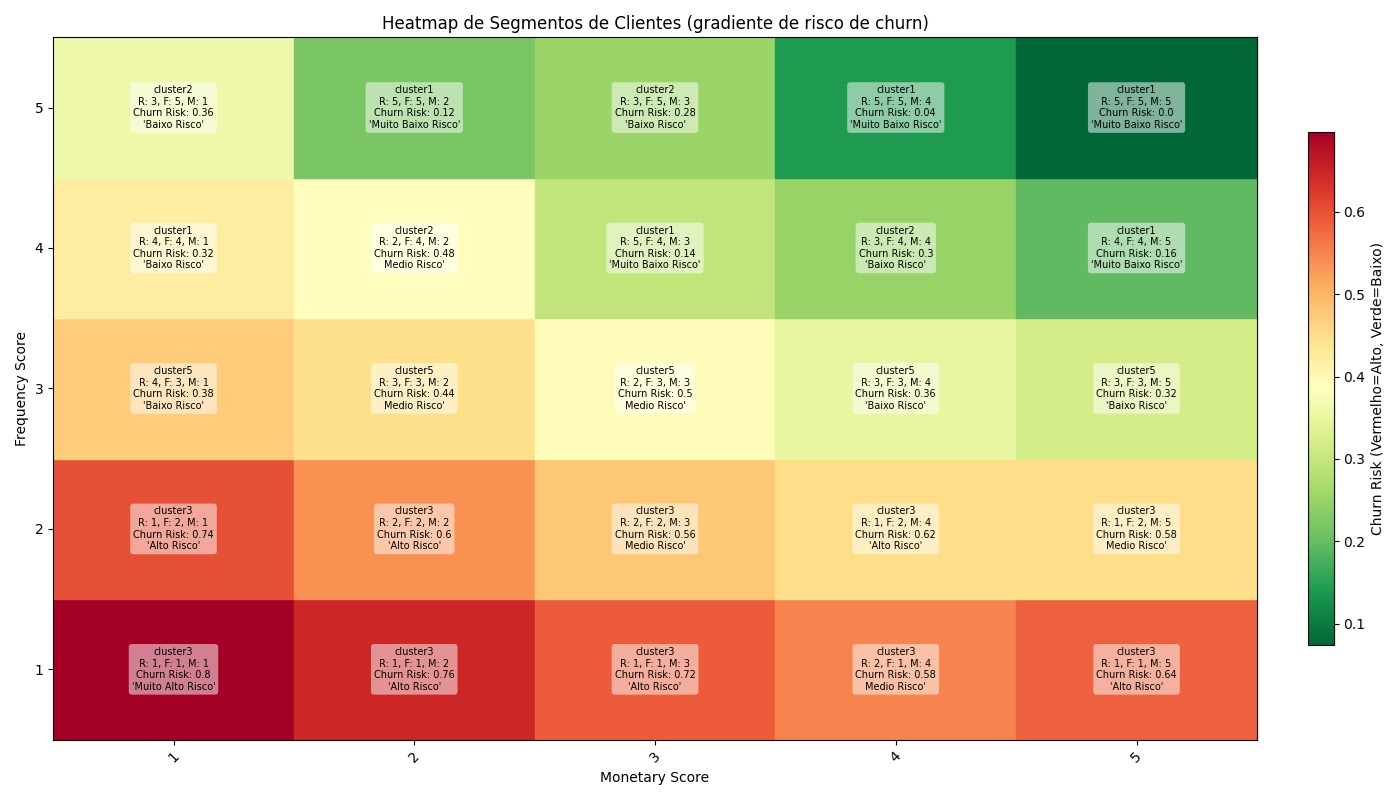
\includegraphics[width=1\linewidth]{imagens/figure29.jpg}\label{cap-5-fig29}
    \captionof{figure}[LOF entry]{Risco de \textbf{\textit{Churn}}, gráfico 2D \textit{Monetary_score vs. Frequency_score}.}
    \label{fig29}
    \end{centering}
\end{figure}

\begin{enumerate}
	\item \textit{\textbf{Cores verdes (Risco mais baixo)}}: Os clientes nas zonas verdes apresentam risco baixo de abandono [0.0 - 0.36]. Estes clientes têm pontuações altas em todas as métricas, sendo clientes com realizam compras com frequência e de alto valor monetário. O seu risco de abandono é baixo, indicando propensão para continuarem a comprar.

Não são clientes preocupantes em termos de risco, no entanto, a implementação de benefícios \textit{premium}, programas de fidelidade ou então recompensas por lealdade irão permitir que estes continuem a realizar compras de futuro e a manter o risco de abandono minimizado.
	\item \textit{\textbf{Cores amarelas (Risco médio)}}: Apresentam um risco médio de abandono [0.48 - 0.5].
Em termos de pontuações, têm níveis de \textbf{Recência} e \textbf{Valor Monetário} mais mais baixos mas valores de \textbf{Frequência} médios/altos. Indicam que realizaram muitas compras, mas o valor monetário das mesmas foi baixo e a data da última compra foi a algum tempo.

Estes clientes são bons alvos para estratégias que incentivem ao consumo, através de descontos para compras de maior valor para aumentar o seu gasto médio. Outro estratégia será a criação de campanhas ou promoções limitadas no tempo, fomentando assim o aumento da sua frequência.
	\item \textit{\textbf{Cores laranja (Risco médio/alto)}}: Apresentam niveis de risco amplos, indo do baixo ao alto risco [0.32 - 0.6].

No caso em que o risco é mais baixo dentro das zonas laranja, correspondem a clientes com pontuações de \textbf{Recência} e \textbf{Frequência} mais elevadas, mas com níveis extremamente baixos de pontuação em \textbf{Valor Monetário}. Estes clientes realizam compras com frequência e no passado recente, no entanto o valor agregado das compras é muito baixo. Deverão ser alvos de estratégias que permita aumentar o valor, como a criação de campanhas direcionadas que ofereçam descontos em produtos de maior valor.

Em casos em que o risco de abandono é mais elevado, a pontuação em termos de \textbf{Valor Monetário} é mais expressiva, no entanto as pontuações de \textbf{Recência} e \textbf{Frequência} são extremamente baixas. Estes clientes realizaram compras ou de baixo valor ou de muito elevado valor no passado, mas realizaram-nas poucas vezes e a última compra foi a muito tempo. Deverão ser alvos de estratégias que permita aumentar a \textbf{Recência} e \textbf{Frequência} para aumentar o comprometimento com a organização e reduzir ainda mais o risco de abandono associado.

	\item \textit{\textbf{Cores vermelhas (Risco muito alto)}}: Estes clientes apresentam um risco de abandono muito elevado [0.64 - 1].
São clientes com pontuações muito baixas em todas as métricas que ou estão em risco muito elevado de inatividade ou já se encontram inativos. 

Deverão ser alvos de campanhas agressivas de \textit{engagement}, como emissão de descontos, campanhas por tempo limitado, mecânismos de fidelização ou outros que permitam aumentar as pontuações de \textbf{Recência}, \textbf{Frequência} e  \textbf{Valor Monetário}.
\end{enumerate}

\begin{figure}[H]
    \begin{centering}
    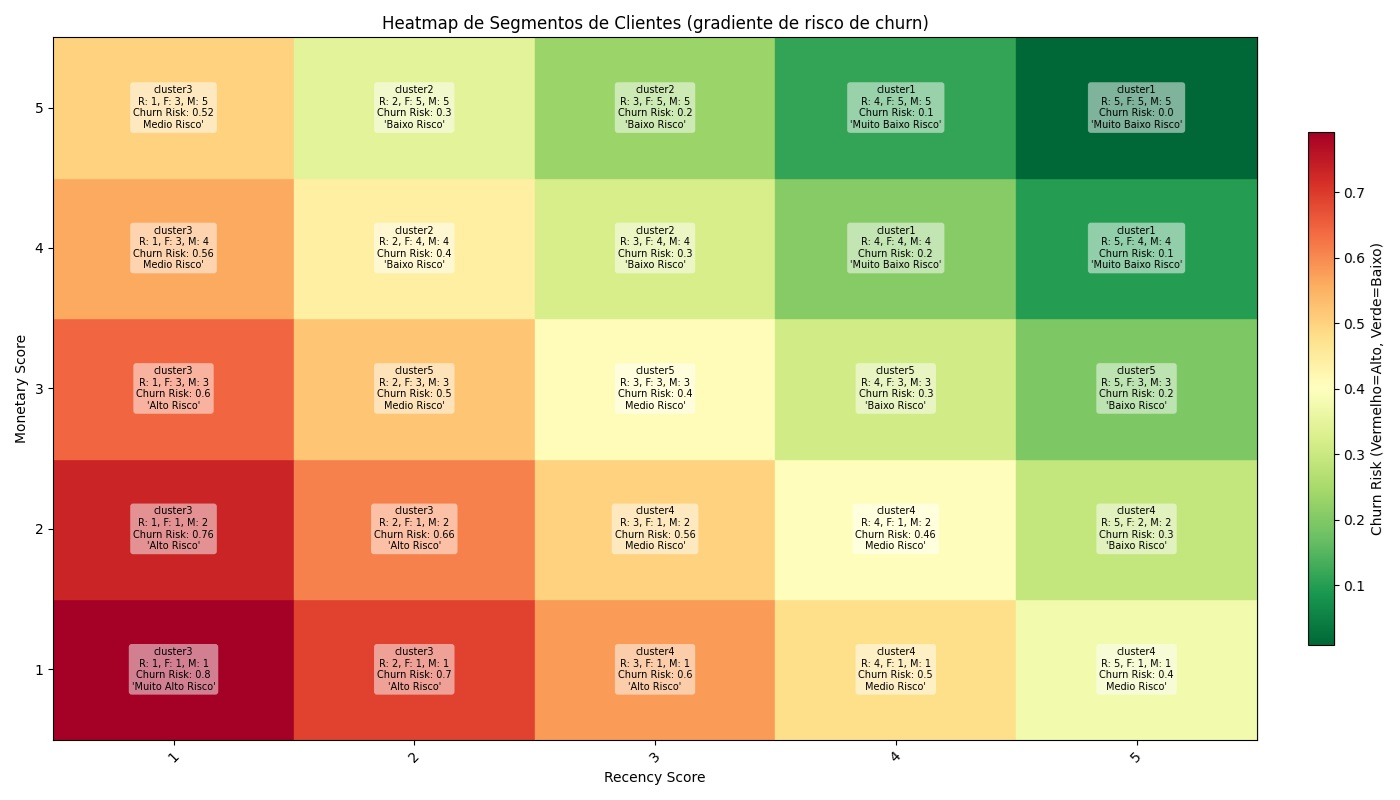
\includegraphics[width=1\linewidth]{imagens/figure30.jpg}\label{cap-5-fig30}
    \captionof{figure}[LOF entry]{Risco de \textbf{\textit{Churn}}, gráfico 2D \textit{Monetary_score vs. Recency_score}.}
    \label{fig30}
    \end{centering}
\end{figure}

\begin{enumerate}
	\item \textit{\textbf{Cores verdes (Risco mais baixo)}}: Estes clientes apresentam o risco mais baixo de abandono [0.0 - 0.3].

Estes clientes são os clientes mais valiosos e leais, compram recentemente e gastam muito. Nas zonas verdes mais perto das zonas amarelas, existem dois tipos de clientes: aqueles que realizaram compras recentemente mas que têm pontuações de \textbf{Frequência} e \textbf{Valor Monetário} ou então os clientes que compravam frequentemente e que gastavam muito, mas que não realizam compras à algum tempo.

Será necessário a implementação de estratégias que permitam diminuir o risco ainda mais, para que estes clientes não sejam segmentados nas outras zonas de maior risco. Exemplos seriam a oferta de benefícios \textit{premium}, como descontos exclusivos e eventos VIP, ou então programas de fidelidade para recompensar a frequência.
	\item \textit{\textbf{Cores amarelas (Risco médio)}}: Apresentam um risco médio de abandono [0.4 - 0.46].

Nestes clientes, quanto maior a pontuação de \textbf{Recência}, menores são as pontuações de \textbf{Frequência} e \textbf{Valor Monetário}. Ou seja, clientes que compraram recentemente, realizaram menos compras e com menor valor, por outro lado, clientes que não realizam compras à algum tempo, quando compravam realizavam-no com alguma frequência e as compras tinham maior valor.

Nestes casos, será vantajosa a realização de um estudo sobre quais os motivos que levaram a esse comportamento, por forma a criar estratégias eficazes que permitam reduzir o risco de abandono e o aumento do \textit{engagement} dos clientes.
	\item \textit{\textbf{Cores laranja (Risco médio/alto)}}: Estes clientes apresentam um risco de abandono mais elevado [0.5 - 0.66].

Estes clientes apresentam um comportamento semelhante aos clientes das zonas amarelas, no entanto o "fosso" entre as pontuações é mais acentuado, o que leva a um aumento do risco.

O estudo aplicado aos clientes situados nas zonas amarelas também é válido aqui, no entanto as estratégias para recuperar/manter estes clientes têm de ser mais agressivas dado o maior risco associado.
	\item \textit{\textbf{Cores vermelhas (Risco muito alto)}}: Os clientes nestas zonas apresentam um risco muito alto de abandono [0.7 - 1], podendo já estar inativos.

São clientes cujas pontuações em todas as métricas são extremamente baixas, devendo ser alvos de campanhas agressivas de \textit{engagement}, como emissão de descontos, campanhas por tempo limitado, mecânismos de fidelização ou outros que permitam aumentar as pontuações de \textbf{Recência}, \textbf{Frequência} e  \textbf{Valor Monetário}.
\end{enumerate}

\newpage
\subsection{Resultados de classificadores}

Antes da realização dos nossos testes, foi necessário proceder a um último ajuste no conjunto de dados, nomeadamente a remoção do atributo \textit{\textbf{ChurnRisk}}. Este atributo, como demonstrado anteriormente representa a probabilidade de risco de abandono, num valor normalizado de 0 a 1. Este deve de ser removido pois a classe é o atributo com nome \textit{\textbf{ChurnRisk_description}} (que representa valores nominais de risco) foi criada com base em regras aplicadas sobre o atributo \textit{\textbf{ChurnRisk}} (ou seja, foi derivada desse atributo). A sua não remoção causaria o chamado \textit{\textbf{data leakage}}, em que a performance dos modelos é artificialmente aumentada (ou digamos, inflacionada), o que leva ao chamado \textit{\textbf{overfitting}}. A remoção deste atributo obriga os nossos classificadores a associarem os níveis de risco às pontuações RFM, efetivamente aprendendo por si as regras de classificação.

Para a realização da avaliação do nosso modelo, foi utilizada uma abordagem intitulada de \textbf{\textit{análise da curva de aprendizagem}} (\textit{learning curve analysis}). Neste tipo de abordagem, é realizada uma separação prévia dos nossos dados num conjunto de teste independente e num conjunto de treino. A percentagem escolhida foi, 20\% para teste e 80\% para treino.

Os dados reservados para treino, foram divididos ainda mais, resultando em parcelas incrementais de 10\%. Ou seja, os dados reservados para treino, foram repartidos em parcelas que vão dos 10 aos 100\% do nosso conjunto de treino que consiste em 80\% do dataset original.

Esta divisão garante que os nossos dados de teste sejam independentes dos dados de treino, mitigando ao máximo ou até mesmo eliminando o risco dos classificadores testados de "memorizarem" as regras de associação, o que iria inflacionar as métricas de desempenho, tornando-as irrealistas e até mesmo falaciosas.


Os dados que foram utilizados são os seguintes:

\begin{enumerate}
	\item \textbf{Dados de Teste}: 20\% do dataset preparado e limpo, num total de 1173 instâncias.
	\item \textbf{Dados de Treino}: 80\% do dataset preparado e limpo, num total de 4690 instâncias. Estas irão ser divididas nas seguintes parcelas usadas como treino:
		\item[\textbullet] Subconjunto de 10\%, num total de 469 instâncias.
		\item[\textbullet] Subconjunto de 20\%, num total de 938 instâncias.
		\item[\textbullet] Subconjunto de 30\%, num total de 1407 instâncias.
		\item[\textbullet] Subconjunto de 40\%, num total de 1876 instâncias.
		\item[\textbullet] Subconjunto de 50\%, num total de 2345 instâncias.
		\item[\textbullet] Subconjunto de 60\%, num total de 2814 instâncias.
		\item[\textbullet] Subconjunto de 70\%, num total de 3283 instâncias.
		\item[\textbullet] Subconjunto de 80\%, num total de 3752 instâncias.
		\item[\textbullet] Subconjunto de 90\%, num total de 4221 instâncias.
		\item[\textbullet] Todo o conjunto de treino, num total de 4690 instâncias.
\end{enumerate}

\newpage
Para a realização dos testes, foram utilizados os seguintes algoritmos:

\begin{enumerate}
	\item \textit{\textbf{J48}}: Algoritmo de classificação baseado em árvores de decisão, a sua utilização de regras lineares torna-o um bom candidato para este tipo de problemas, em que níveis de pontuação RFM estão associadas a riscos de abandono (\textit{\textbf{Churn}}) específicos. A sua estrutura baseada em árvores de decisão torna muito fácil a interpretação das suas regras, no entanto é propenso à ocorrência de \textit{overfitting}, principalmente em conjuntos de dados com ruído. Em termos de dimensionalidade, não é adequado a conjuntos de dados muito extensos, pois a árvore de decisão pode tornar-se demasiado complexa.
	\item \textit{\textbf{RandomForest}}: Este algoritmo de classificação também é baseado em árvores de decisão, mas enquanto o \textit{J48} gera uma única árvore, o \textit{RandomForest} combina múltiplas árvores de decisão. É eficaz na redução do fenómeno de \textit{overfitting}, e funciona bem com em conjuntos de dados com alta dimensionalidade (tanto em número de atributos como de instâncias).
	\item \textit{\textbf{Logistic}}: Este algoritmo de classificação, também denominado de \textbf{regressão logística}, é um algoritmo muito rápido e eficiente. Funciona bem em dados com separações lineares.
	\item \textit{\textbf{SMO}}: Este algoritmo de classificação também é conhecido como \textit{\textbf{Support Vector Machine with Sequential Minimal Optimization}}. É eficaz para dados com elevada dimensionalidade, funciona bem quando na presença de relações não lineares e é robusto contra o \textit{overfitting}.
	\item \textit{\textbf{IBk}}: Este algoritmo, conhecido como \textit{\textbf{K-Nearest Neighbour}} realiza previsões com base na similaridade com vizinhos, não exige fase de treino do modelo e pode capturar relações não lineares nos dados. Foi demonstrado anteriormente que o risco de abandono está dependente das pontuações RFM e que não existem grandes saltos de pontuações entre zonas (apenas incrementos ou decrementos de 1), logo, existe similaridade entre zonas vizinhas pois os valores entre zonas nunca são muito dispares. Como tal, o IBk foi escolhido como bom candidato para os testes.
\end{enumerate}

\underline{\textit{\textbf{Nota}}}: Todos os algoritmos acima foram testados no \textit{software} \textit{\textbf{Weka}}, versão 3.8.6, com os valores por defeito.


\begin{figure}[H]
    \begin{centering}
    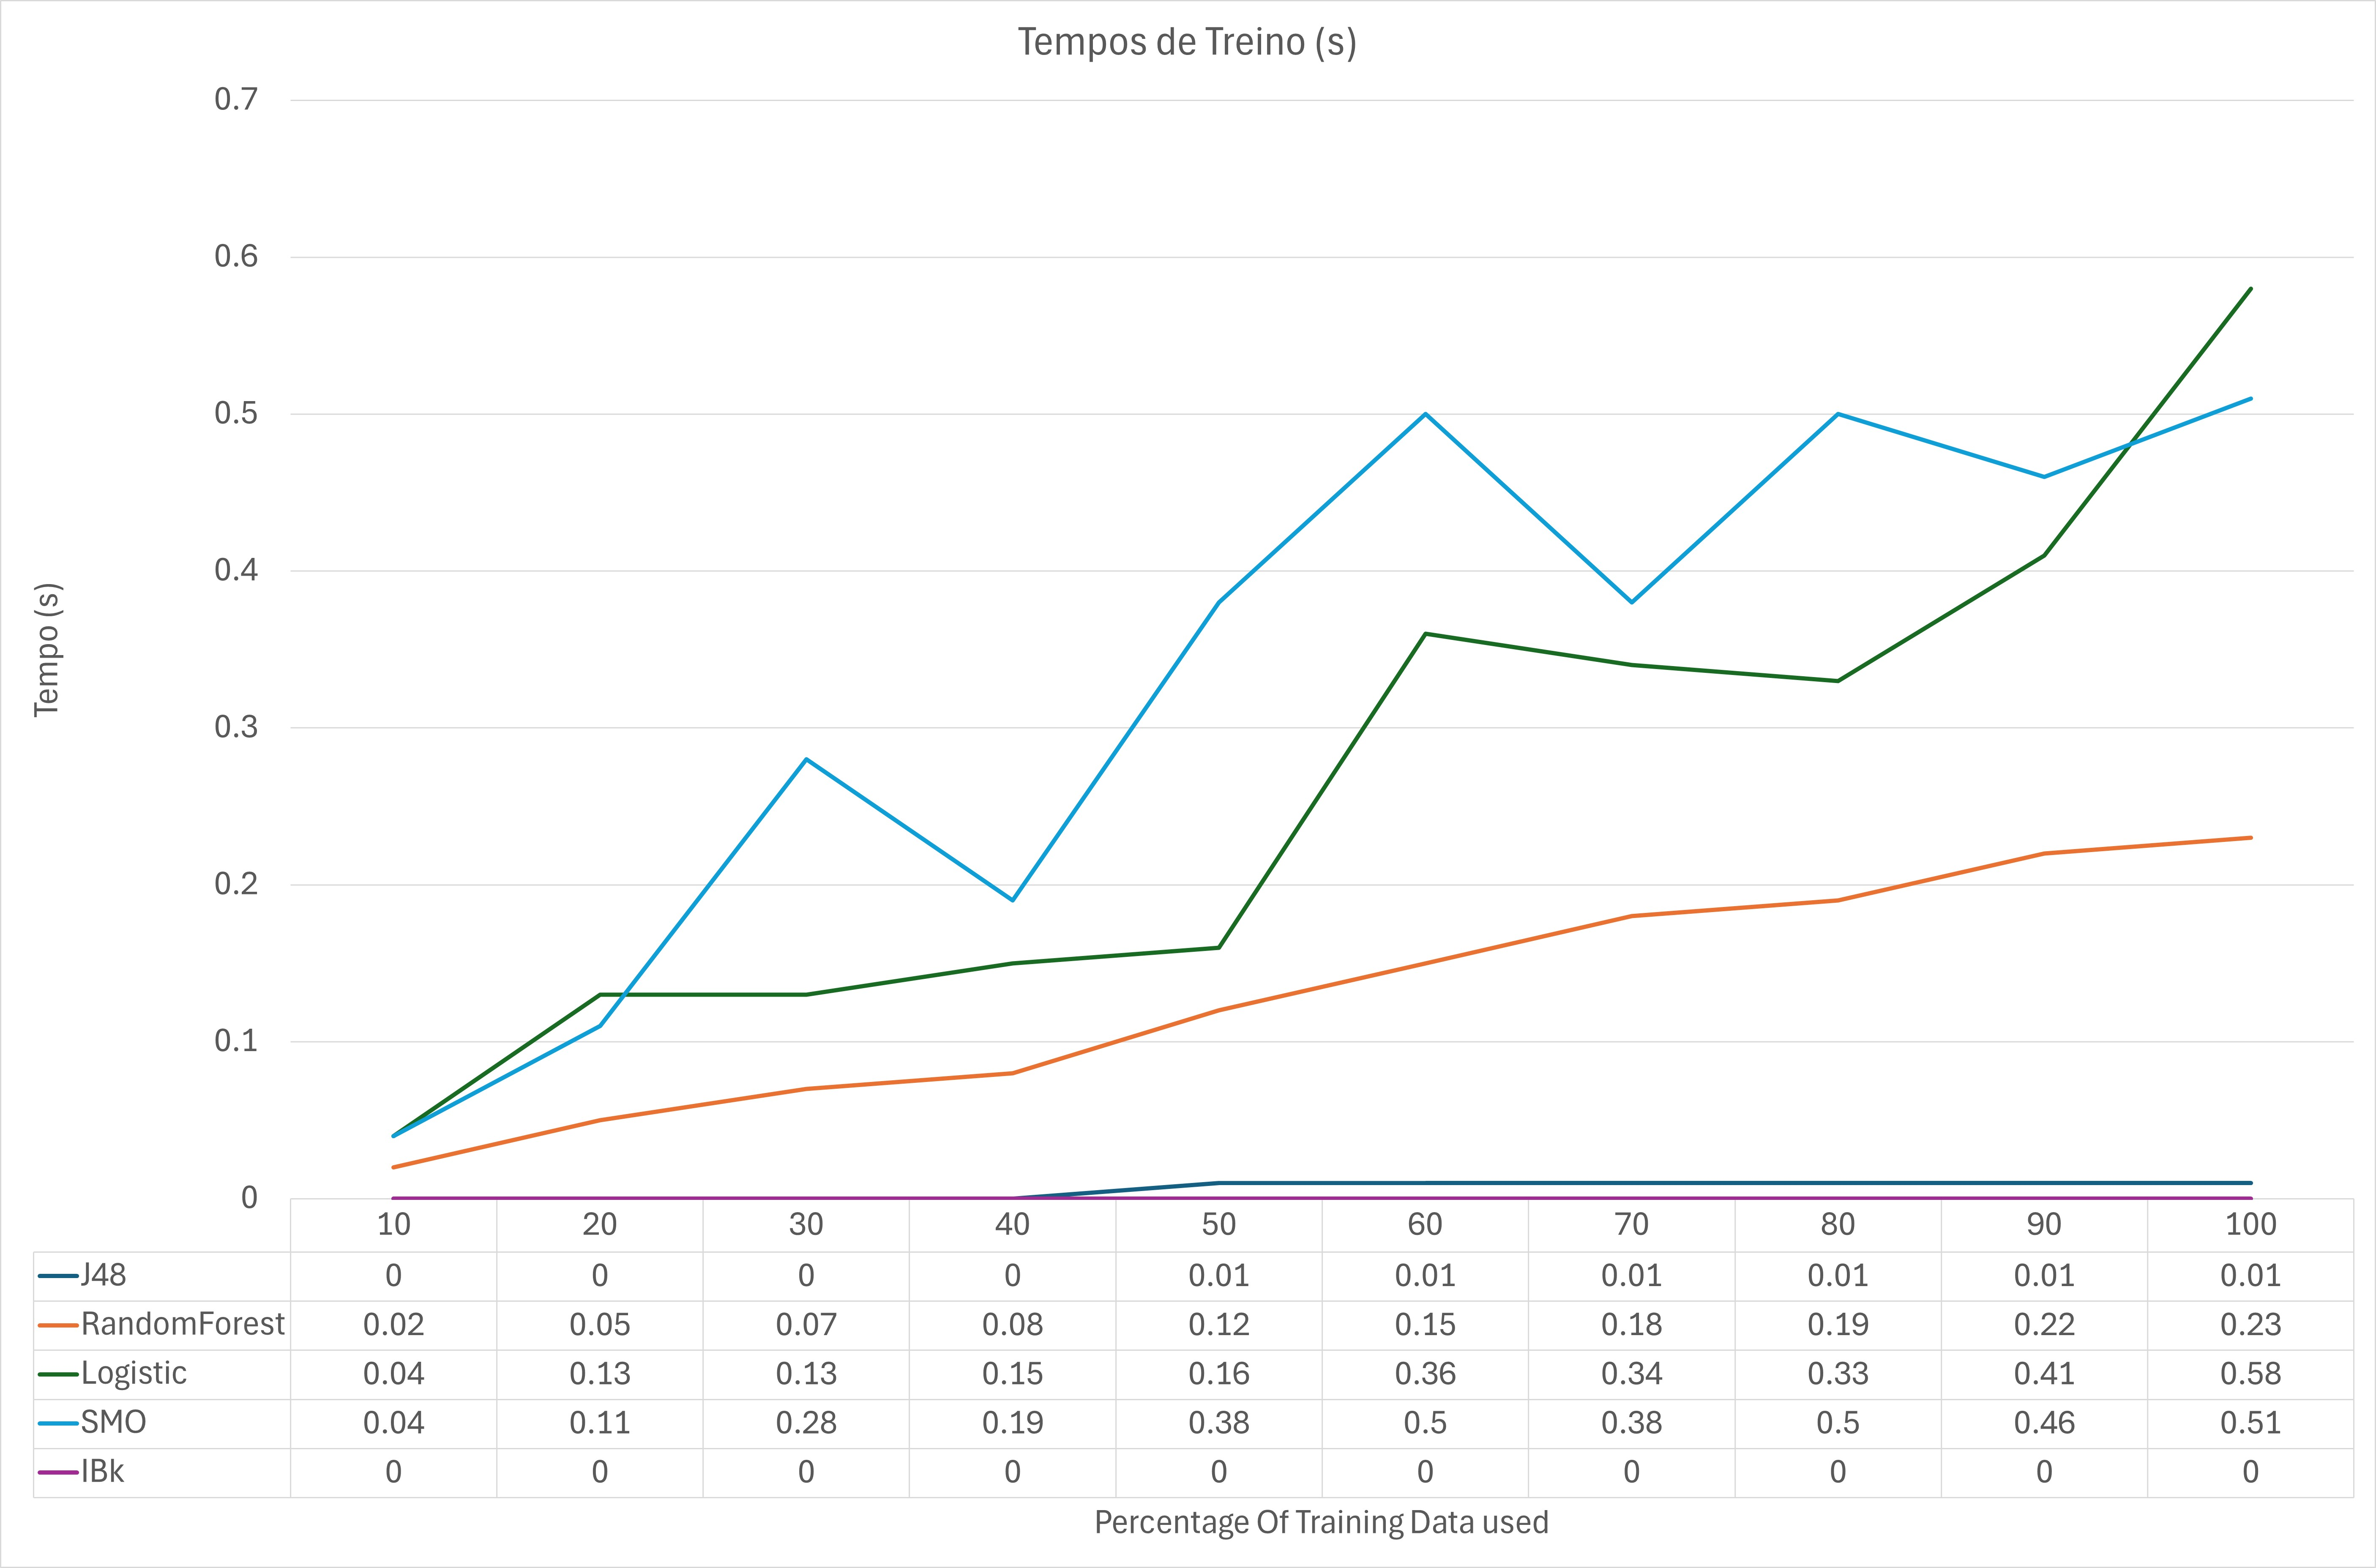
\includegraphics[width=1\linewidth]{imagens/figure38.jpg}\label{cap-5-fig38}
    \captionof{figure}[LOF entry]{Comparação dos tempos de treino dos algoritmos, por \textit{training splits}.}
    \label{fig38}
    \end{centering}
\end{figure}

\begin{figure}[H]
    \begin{centering}
    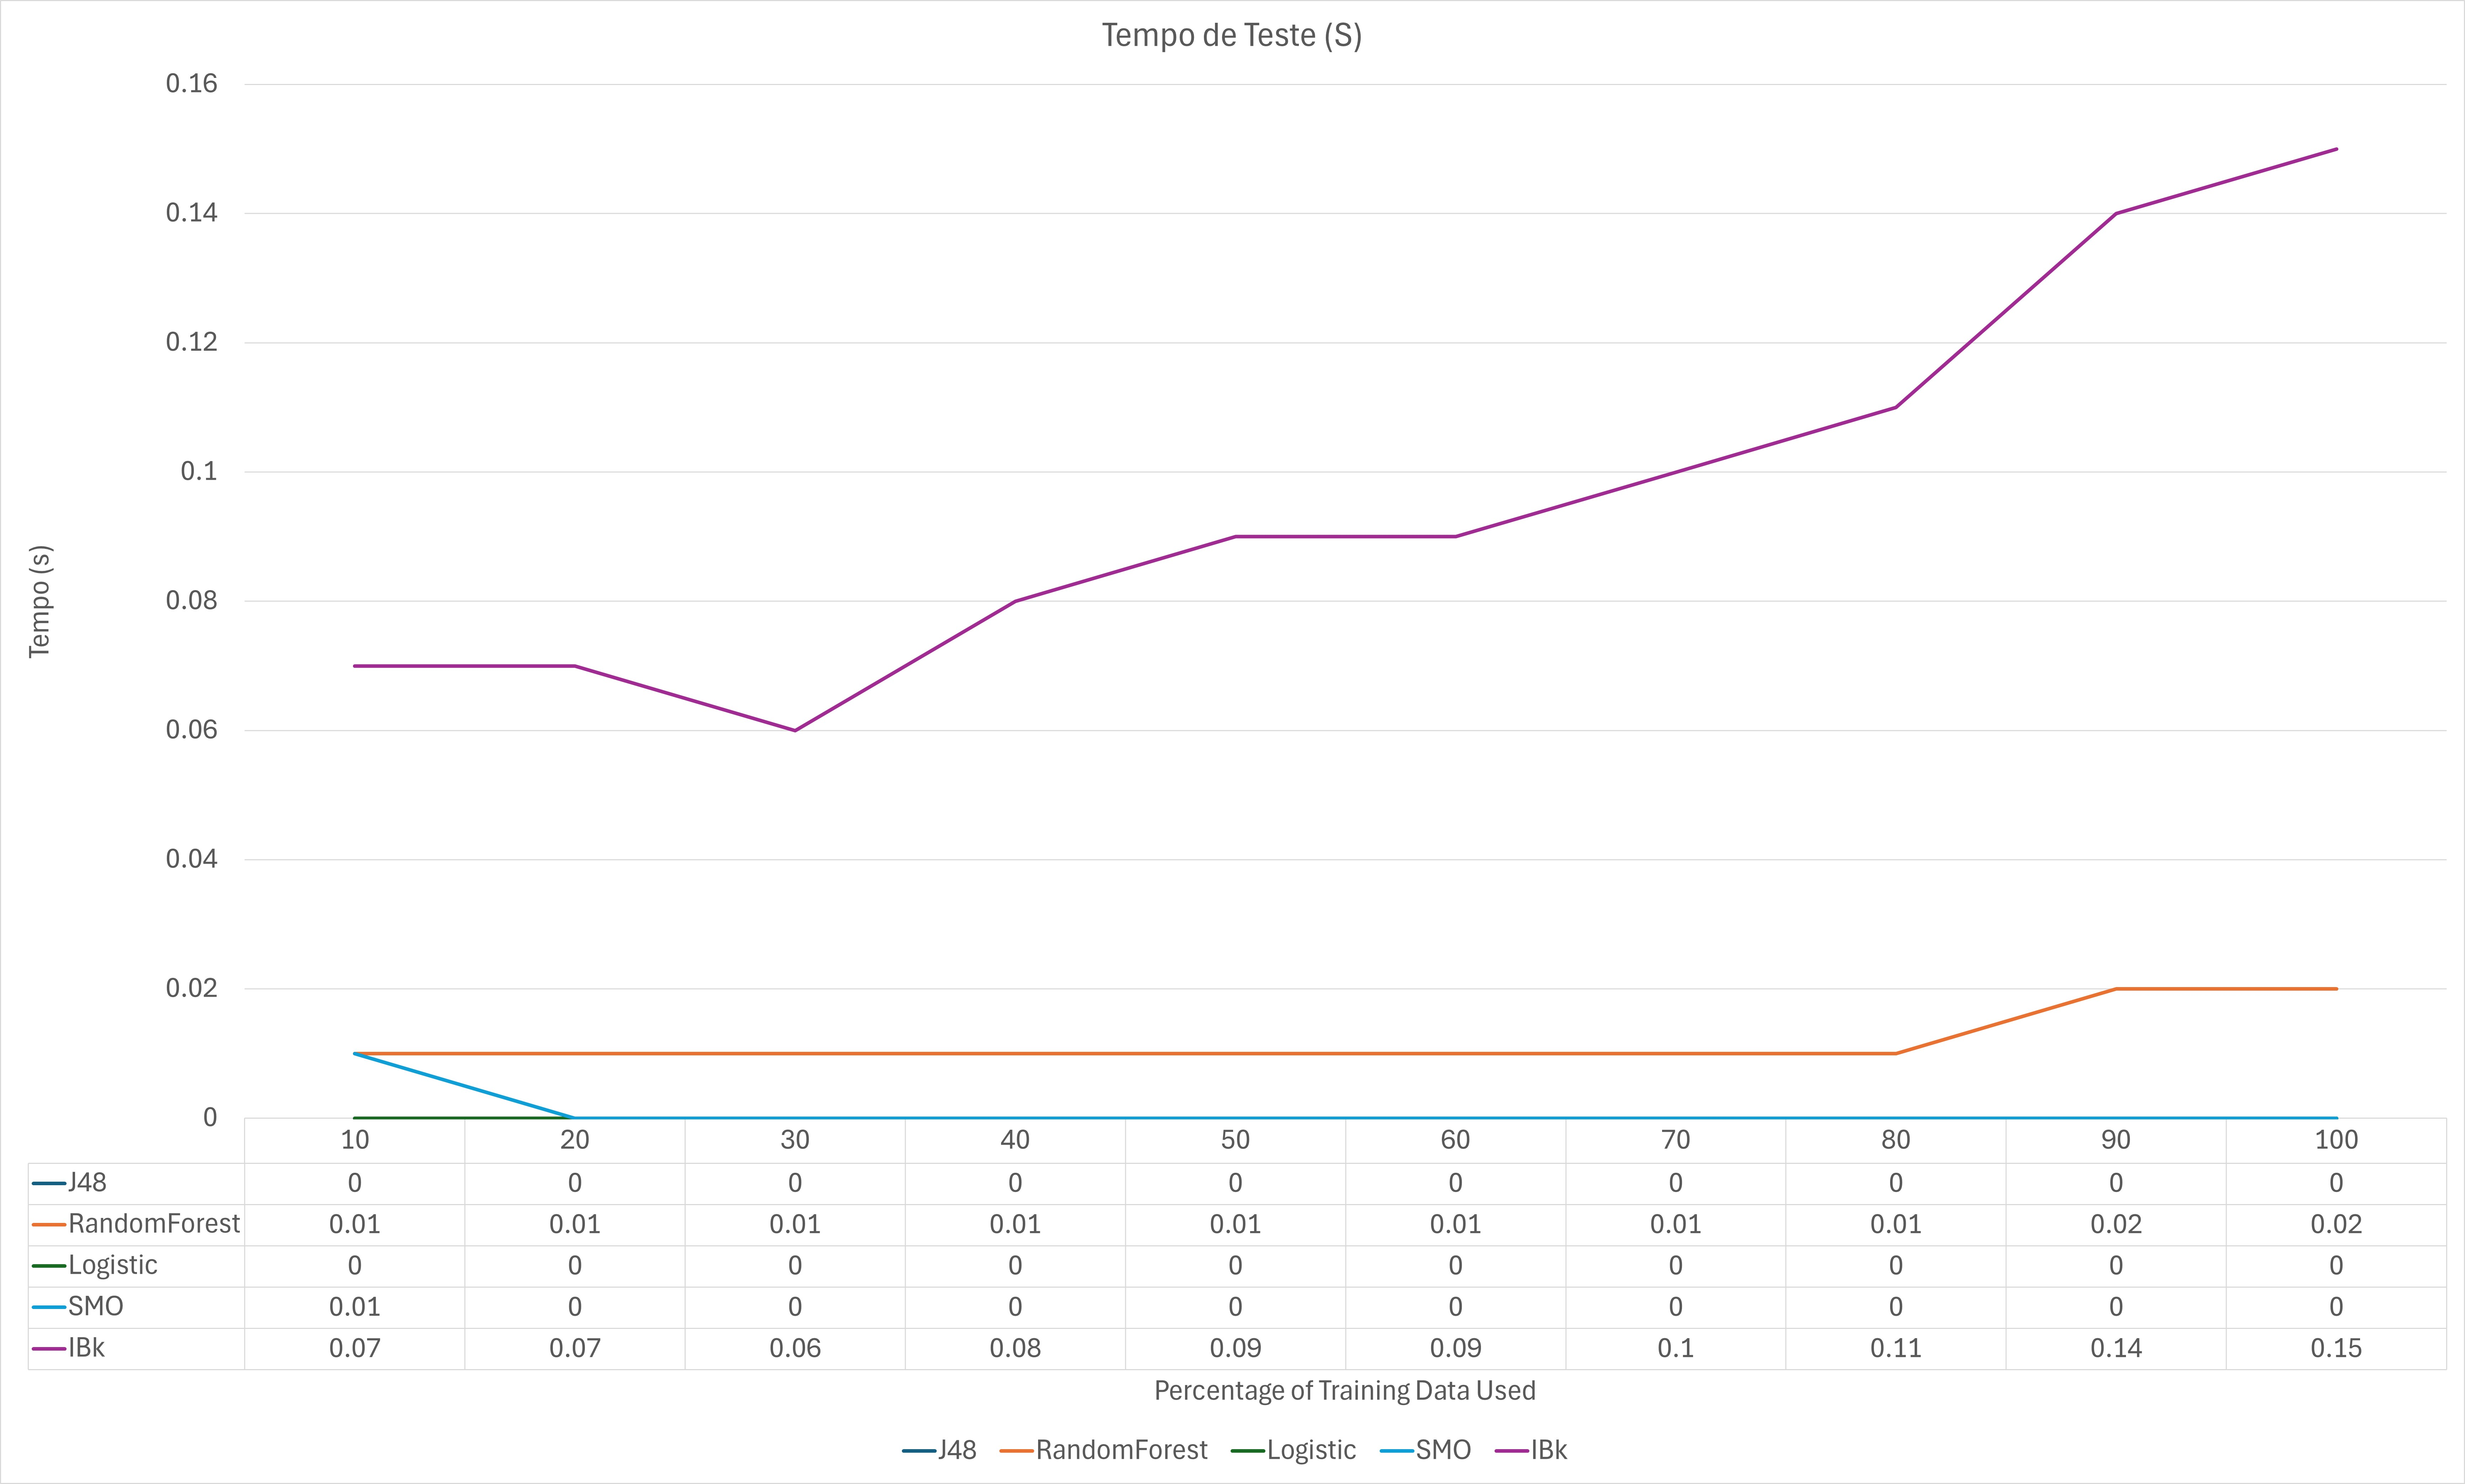
\includegraphics[width=1\linewidth]{imagens/figure39.jpg}\label{cap-5-fig39}
    \captionof{figure}[LOF entry]{Comparação dos tempos de teste dos algoritmos, por \textit{training splits}.}
    \label{fig39}
    \end{centering}
\end{figure}

Os gráficos acima ilustram a variação dos tempos de treino e teste para cada um dos classificadores, em função da percentagem de dados de treino utilizados. Verifica-se o seguinte:

\begin{enumerate}
	\item \textbf{\textit{J48}}: 
		\item[\textbullet] \textbf{Tempo de Treino}: Os tempos de treino são quase nulos em todas as percentagens de dados de treino, isso pode ser explicado pela natureza do classificador \textbf{\textit{J48}}, que constrói árvores de decisão com base na divisão dos dados de treino em subconjuntos, através de divisões recursivas até que sejam atingidos nós folha ou critérios de paragem. Este processo, embora recursivo é computacionalmente muito eficiente em comparação com outros algoritmos. Além disso, o \textit{\textbf{J48}} é altamente otimizado para conjuntos de dados de tamanho pequeno, com número limitado de instâncias e atributos, terminando rapidamente pois não são realizados cálculos excessivamente complexos.
		\item[\textbullet] \textbf{Tempo de Teste}: Os tempos de teste são praticamente nulos em todas as percentagens de dados de treino. Isso pode mais uma vez ser explicado pela natureza do classificador, em que, após o treino, uma árvore de decisão é construída e podada. Essa estrutura é hierárquica e segue um fluxo determinístico, no qual cada instância percorre a àrvore a partir da raiz até chegar a uma folha. Sendo que o processo de classificação para cada instância apenas consiste na avaliação de condições lógicas em cada nó até chegar a uma folha, o que é extremamente rápido.
	\item \textbf{\textit{Random Forest}}:
		\item[\textbullet] \textbf{Tempo de Treino}: Os tempos de treino são maiores em comparação com o \textit{\textbf{J48}}, mas ainda são relativamente eficientes para a maioria dos cenários. Eles aumentam à medida que a percentagem de dados de treino cresce, devido às características e etapas envolvidas na construção de uma floresta de decisão.

O \textbf{\textit{Random Forest}} é um algoritmo de \textit{ensemble learning} que constrói múltiplas árvores de decisão (geralmente centenas). Cada árvore é construída num subconjunto aleatório do conjunto de treino (o chamado \textit{bagging}). Essa estrutura melhora a robustez do modelo, mas também aumenta o custo computacional do treino, em que o número de árvores da floresta é o maior determinante do tempo de treino. 
		\item[\textbullet] \textbf{Tempo de Teste}: Os tempos de teste do algoritmo são extremamente baixos e praticamente constantes em diferentes tamanhos do conjunto de treino. Essa eficiência pode ser explicada pelas características do algoritmo.

Após o treino, o \textbf{\textit{Random Forest}} armazena todas as àrvores de decisão construídas. Na classificação de novas instâncias, estas são passadas por cada árvore que dará a sua própria previsão. No fim, as previsões são combinadas por votação maioritária e é devolvida a previsão mais votada.

Este processo é extremamente rápido pois à semelhança do \textbf{\textit{J48}}, cada árvore realiza uma busca hierárquica baseada em condições simples até que seja atingido um nó folha ou condição de paragem.
	\item \textbf{\textit{Logistic}}: 
		\item[\textbullet] \textbf{Tempo de Treino}: Os tempos de treino do \textit{Logistic} aumentam gradualmente com o tamanho do conjunto de treino, refletindo o custo computacional do algoritmo para ajustar os pesos e coeficientes durante o processo de otimização. A regressão logística é um modelo linear que utiliza uma função logística para prever probabilidades de classes. Durante o treino, o algoritmo ajusta os coeficientes para minimizar a diferença entre as previsões do modelo e os valores reais. Como tal, o tempo de treino é proporcional ao número de instâncias e ao número de iterações necessárias para que o processo de otimização converja. À medida que o número de dados cresce, mais operações matemáticas têm de ser realizadas, aumentando o tempo.
		\item[\textbullet] \textbf{Tempo de Teste}: Os tempos de teste do \textit{Logistic} são extremamente baixos (no caso deste conjunto de dados, são nulos). Isto é esperado devido à maneira como a regressão logística realiza previsões aós o modelo ser treinado. Durante o teste, o \textit{Logistic} utiliza os parâmetros aprendidos durante o treino para calcular a probabilidade de uma instância pertencer a uma determinada classe. Este processo é computacionalmente leve, consistindo em operações matemáticas básicas como somas, multiplicações, e a aplicação de uma função sigmóide.
	\item \textbf{\textit{SMO}}: 
		\item[\textbullet] \textbf{Tempo de Treino}: Os tempos de treino do \textit{SMO} podem variar significativamente e geralmente aumentam à medida que o tamanho do conjunto de treino cresce. Tal se deve à natureza do algoritmo e às suas características matemáticas. O \textit{SMO} é altamente sensível ao tamanho do conjunto de treino, com o tempo a aumentar quadraticamente ou cubicamente com o número de instâncias e dependendo do \textit{kernel} utilizado.
		\item[\textbullet] \textbf{Tempo de Teste}: Os tempos de teste do \textit{SMO} são baixos e praticamente constantes no gráfico. Após o modelo ser treinado, o \textit{SMO} utiliza os \textbf{vetores de suporte} encontrados durante o treino para classificar novas instâncias. Com o aumento do tamanho do conjunto de treino, o número de vetores de suporte não aumenta significativamente em muitos casos, especialmente se os dados forem separáveis. Desse modo, o tempo de teste permanece quase constante em cada instância.
	\item \textbf{\textit{IBk}}: 
		\item[\textbullet] \textbf{Tempo de Treino}: Os tempos de treino do \textit{IBk} são praticamente inexistentes ou nulos. Tal ocorre pois o \textit{IBk} não realiza um treino convencional, em vez disso, ele simplesmente armazena os dados de treino para uso posterior durante a classificação (daí ser considerado um método \textit{lazy}). 
		\item[\textbullet] \textbf{Tempo de Teste}: Os tempos de teste do \textit{IBk} aumentam proporcionalmente ao tamanho do conjunto de treino. isso ocorre pois o \textit{IBk} calcula as distâncias entre cada nova instância de teste e todas as instâncias do conjunto de treino para determinar os k-vizinhos mais próximos. A sua complexidade computacional depende to número de instâncias de treino e do número de instâncias do conjunto de teste. 
\end{enumerate}


\begin{figure}[H]
    \begin{centering}
    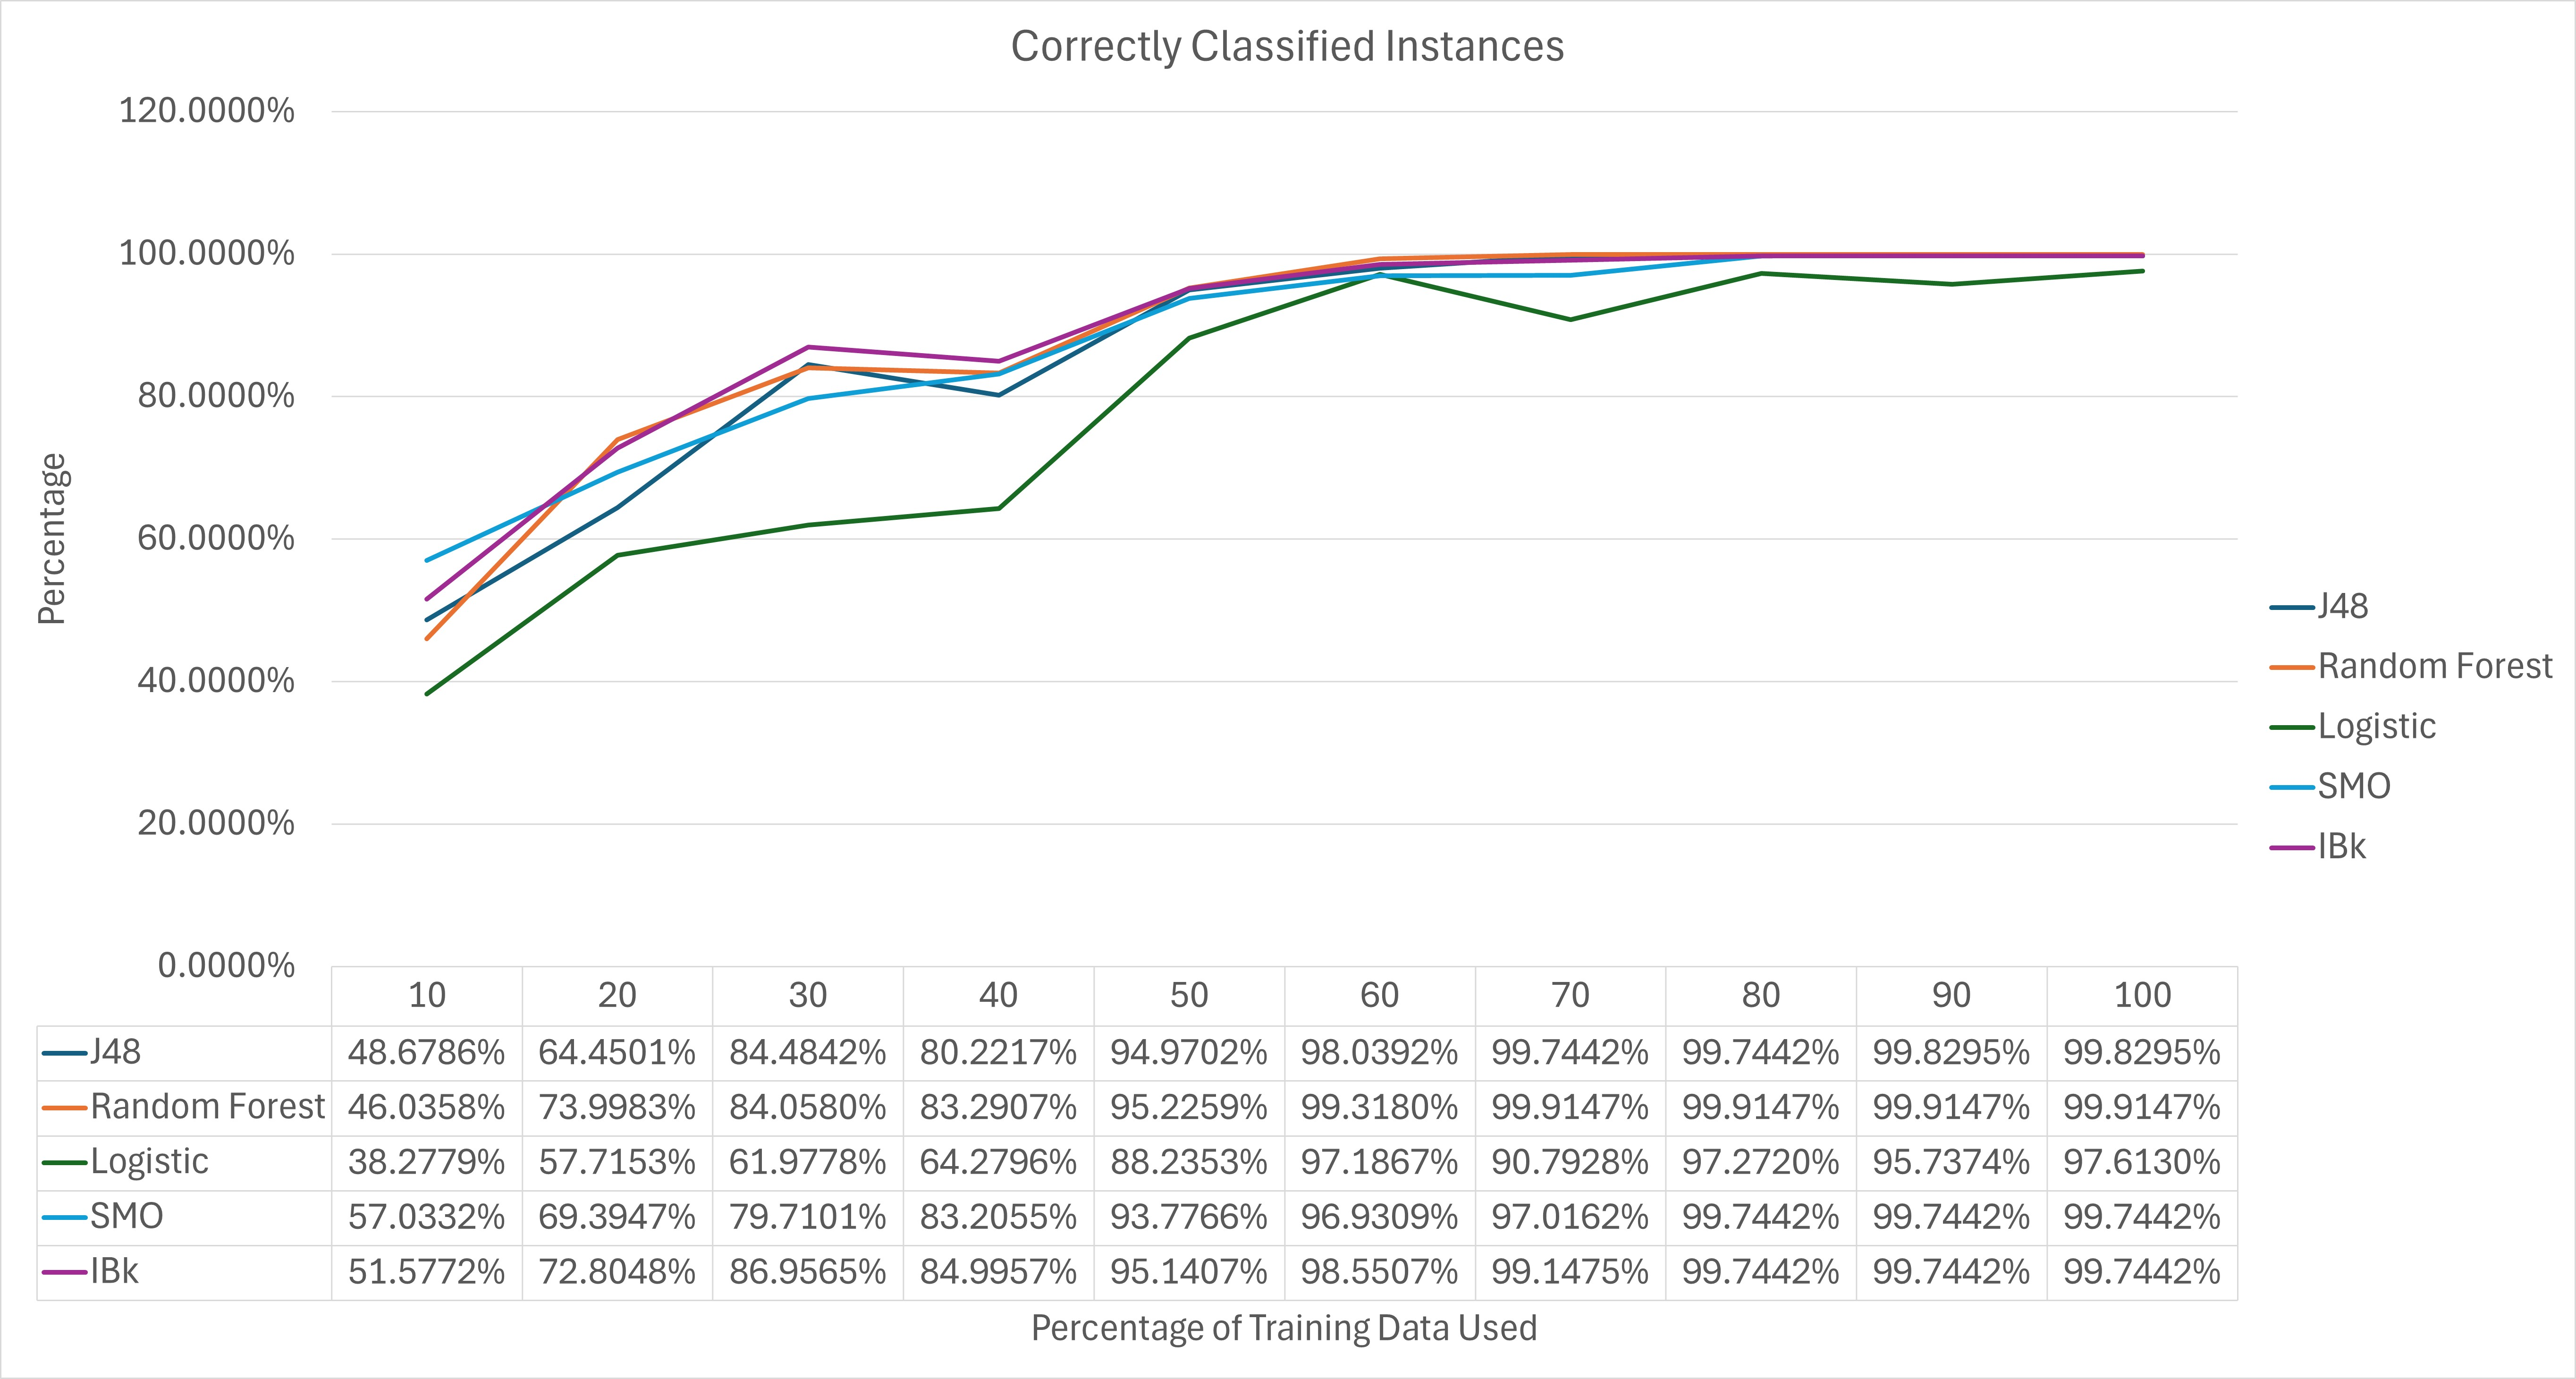
\includegraphics[width=1\linewidth]{imagens/figure32.jpg}\label{cap-5-fig32}
    \captionof{figure}[LOF entry]{Comparação entre percentagem de instâncias corretamente classificadas por \textit{training splits}.}
    \label{fig32}
    \end{centering}
\end{figure}

Com base no gráfico acima, mostrando a evolução no número de instâncias corretamente classificadas, verifica-se o seguinte:

\begin{enumerate}
	\item \textbf{\textit{J48}}: Desempenho semelhante ao \textit{RandomForest}, no entanto para conjuntos de treino mais pequenos os resultados obtidos apresentam alguma inconsistência. Converge para valores muito altos de \textit{performance} (~99.8\%) quando são utilizados conjuntos de treino progressivamente maiores, atingindo o valor mais alto a partir de 70\% dos dados de treino.
	\item \textbf{\textit{Random Forest}}: Grande aumento de desempenho com a utilização de conjuntos de treino progressivamente maiores, convergindo para ~99.91\% de instâncias corretamente classificadas com apenas 70\% dos dados de treino utilizados.
	\item \textbf{\textit{Logistic}}: Foi o classificador com pior desempenho, especialmente com a utilização de conjuntos de treino pequenos em que a utilização de 40\% dos dados de treino apenas atingiu ~64\% de número de instâncias corretamente classificadas, enquanto os restantes classificadores já atingiam valores superiores a 83\%. Com o aumento dos dados de treino, houve um aumento gradual da sua performance, mas continuou sempre abaixo da performance atingida por modelos não lineares, como \textbf{SMO} e \textbf{RandomForest}.
	\item \textbf{\textit{SMO}}: Este classificador apresentou \textit{performance} sólida mas demorou mais tempo a convergir. Atingiu os ~99.7\% de instâncias corretamente classificadas com a utilização de 80\% dos dados de treino.
	\item \textbf{\textit{IBk}}: Foi o classificador com a convergência mais rápida, atingindo ~86\% de instâncias corretamente classificadas utilizando apenas 30\% do conjunto de treino. 
\end{enumerate}

De acordo com o gráfico, todos os classificadores escolhidos melhoraram a sua \textit{performance} à medida que o tamanho do conjunto de treino aumentou. O \textit{\textbf{SMO}} e o \textit{\textbf{Logistic}} apresentaram ritmos de convergência mais lentos quando comparados com os  restantes, que demonstraram ser mais robustos e eficazes com a utilização de dados limitados.

\newpage

\begin{figure}[H]
    \begin{centering}
    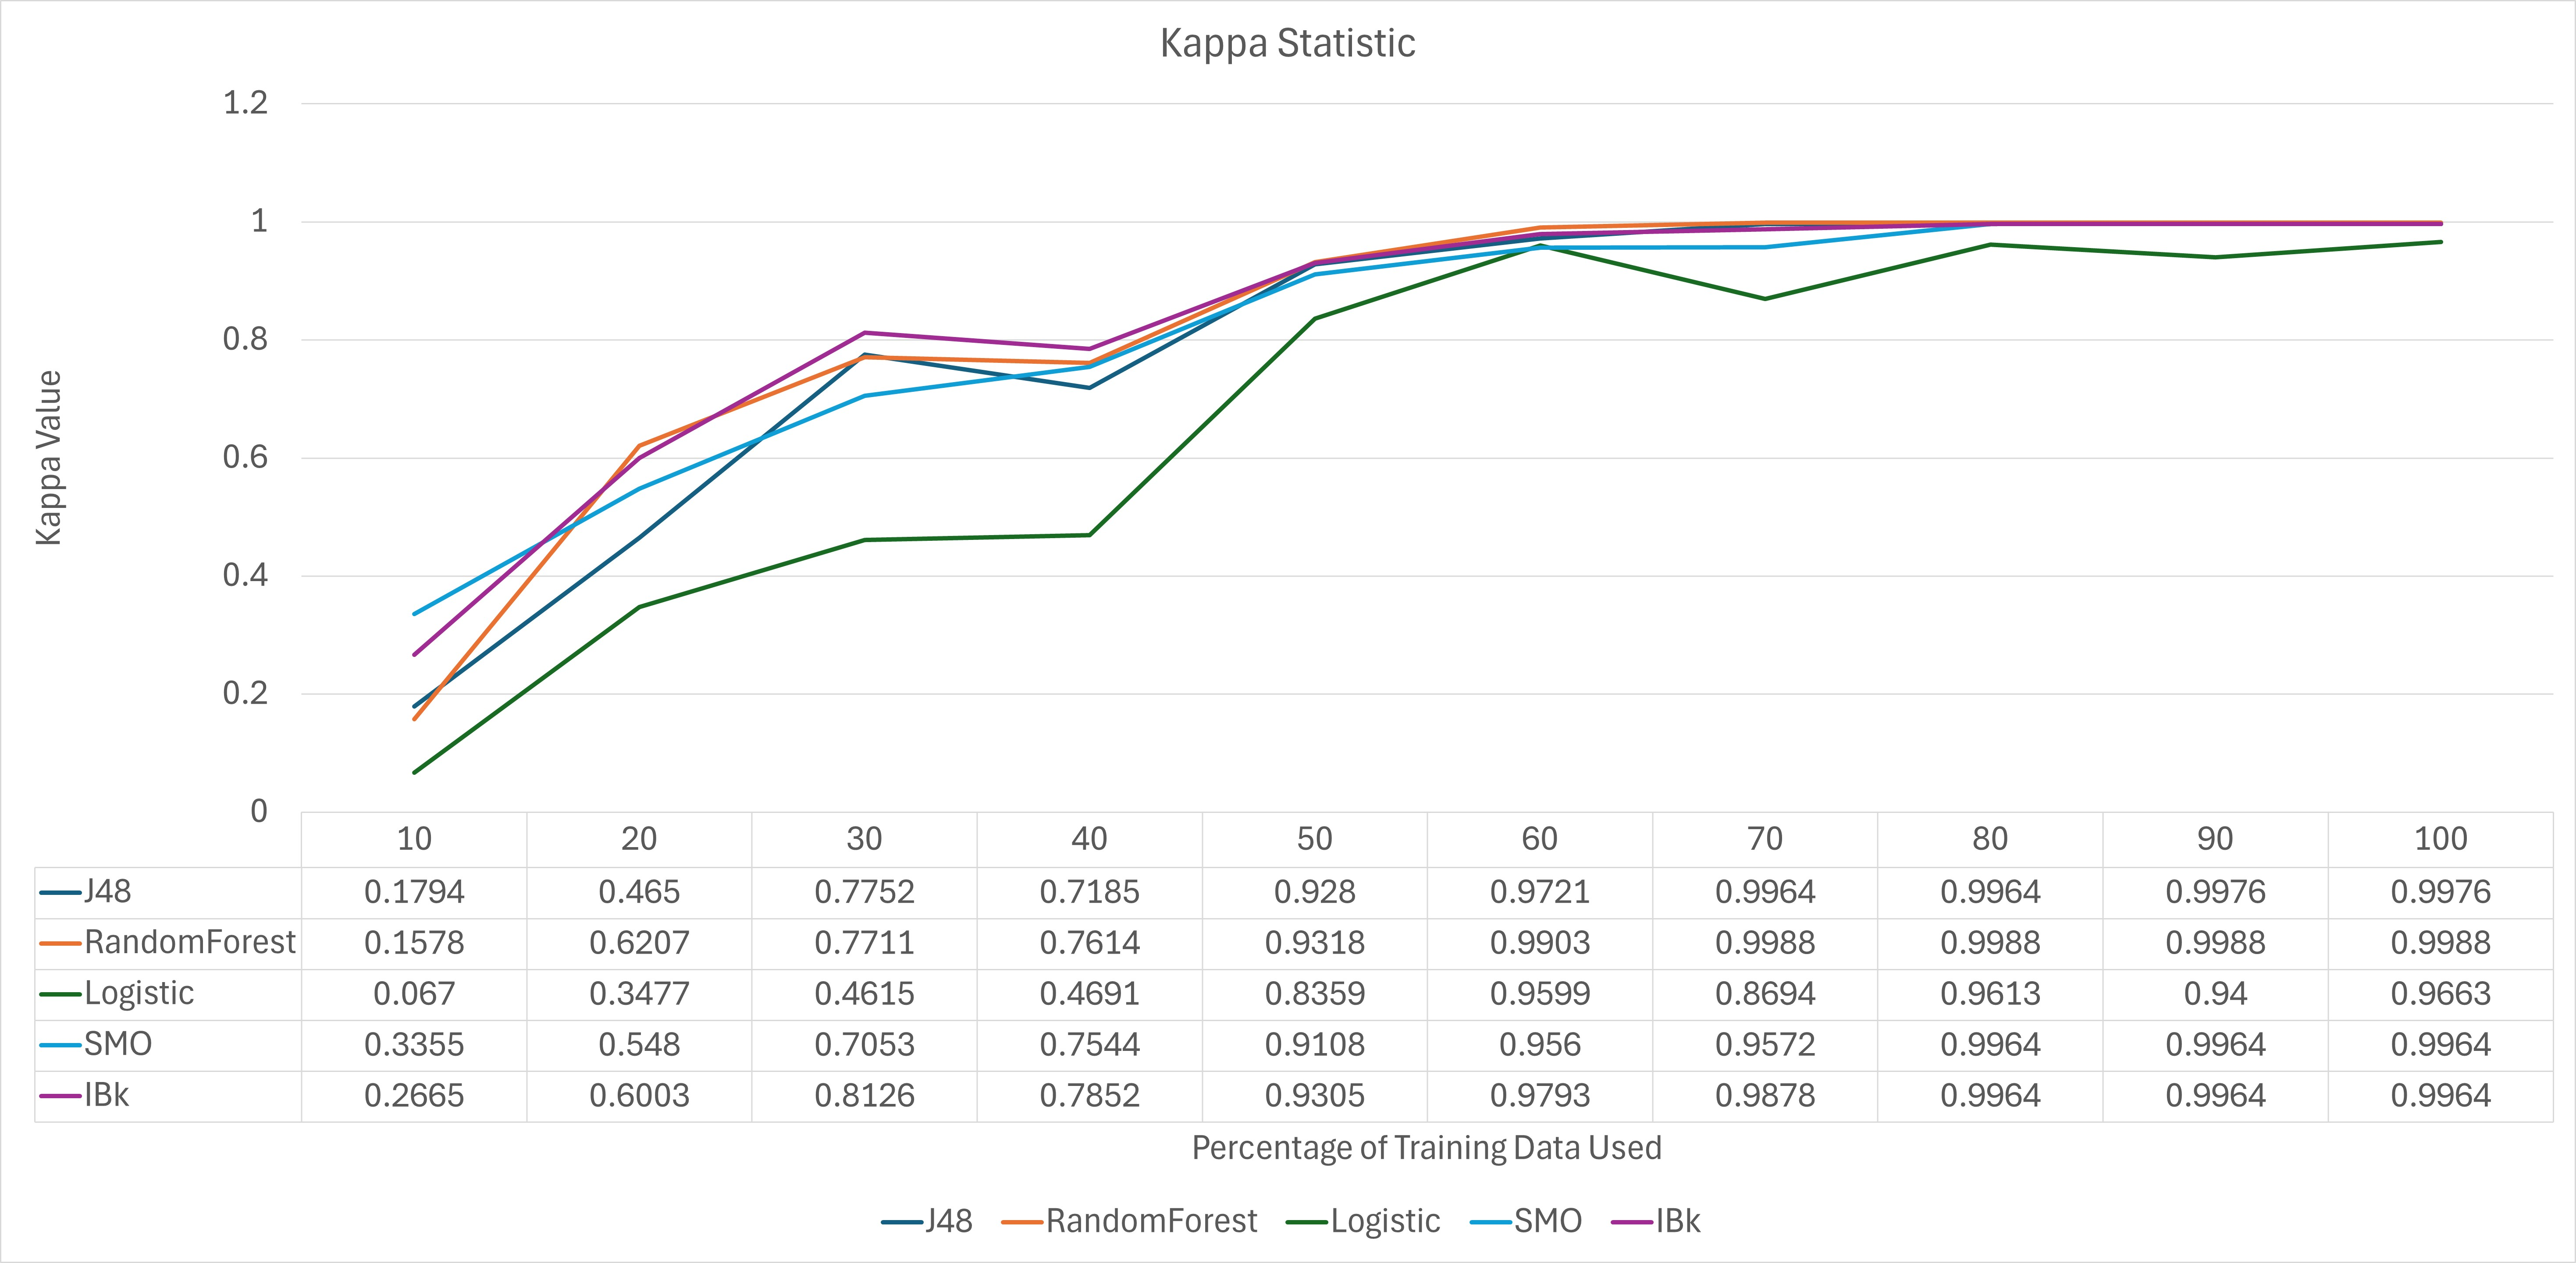
\includegraphics[width=1\linewidth]{imagens/figure33.jpg}\label{cap-5-fig33}
    \captionof{figure}[LOF entry]{Comparação de valores de estatística \textit{Kappa} de cada algoritmo, por cada \textit{training split}.}
    \label{fig33}
    \end{centering}
\end{figure}

A estatística \textit{Kappa} é utilizada para medir a concordância entre as classes previstas e as atuais, com valores perto de 0 indicando que o modelo não é melhor que uma previsão aleatória, e valores perto de 1 que indicam que o modelo é perfeito. Analisando o gráfico, podemos verificar o seguinte:

\begin{enumerate}
	\item \textbf{\textit{J48}}: O classificador \textit{\textbf{J48}} apresentou inicialmente valores de desempenho moderados, tendo uma subida acentuada a partir da utilização de 50\% do conjunto de treino. A partir da utilização de 70\% dos dados de treino, atingiu um planalto em termos de ganhos, mantendo a estatística \textit{Kappa} em ~0.99 com apenas ganhos negligenciáveis. Com dados suficientes, consegue igualar o desempenho dos melhores classificadores.
	\item \textbf{\textit{Random Forest}}: O classificador \textit{\textbf{Random Forest}} apresentou valores superiores logo a partir da utilização de 20\% do conjunto de treino (~0.62). A partir da utilização de 70\% dos dados de treino, foi atingido um planalto em termos de ganhos, mantendo sempre o valor de 0.9988.
	\item \textbf{\textit{Logistic}}: Este classificador tem maus resultados quando o conjunto de treino é muito pequeno, provavelmente devido à sua dependência em relações lineares nos dados. Em termos de convergência, embora tenha atingido um valor elevado (0.9663), continua a ser o algoritmo com menor pontuação, tendo revelado flutuações no valor \textit{\textbf{Kappa}} à medida que o tamanho do conjunto de treino aumentava
	\item \textbf{\textit{SMO}}: Este classificador apresentou o maior resultado inicial em termos de estatística \textit{Kappa}, melhorando de forma contínua com conjuntos de treino progressivamente superiores. Em termos de convergência, atingiu o seu valor máximo(0.9964) nos 80\% do conjunto de treino.
	\item \textbf{\textit{IBk}}: O classificador \textit{\textbf{IBk}} apresentou um comportamento de convergência muito rápido, atingindo o valor \textit{Kappa} de 0.6 a partir dos 20\% do conjunto de treino. Com a utilização de mais dados, apresentou uma subida constante, tendo atingido o planalto nos 80\% do conjunto de treino. 
\end{enumerate}

De acordo com o gráfico, todos os classificadores escolhidos apresentaram valores de \textit{\textbf{Kappa}} muito elevados, com a maioria a atingir valores acima dos 0.99, com apenas o \textit{\textbf{Logistic}} a ficar pelos 0.96.
Os classificadores \textbf{RandomForest} e \textbf{IBk} apresentam valores desempenho elevados por todas as percentagens de treino, indicando que são escolhas robustas para tarefas de classificação. O \textbf{SMO} também é boa escolha, mas requer mais dados.

O classificador \textbf{Logistic} tem dificuldades inicialmente devido à sua assunção de linearidade, mas vai-se tornando mais eficaz com mais dados. Modelos não lineares como \textbf{Random Forest}, \textbf{SMO} e \textbf{IBk} conseguem lidar melhor com a complexidade do conjunto de dados.

\begin{figure}[H]
    \begin{centering}
    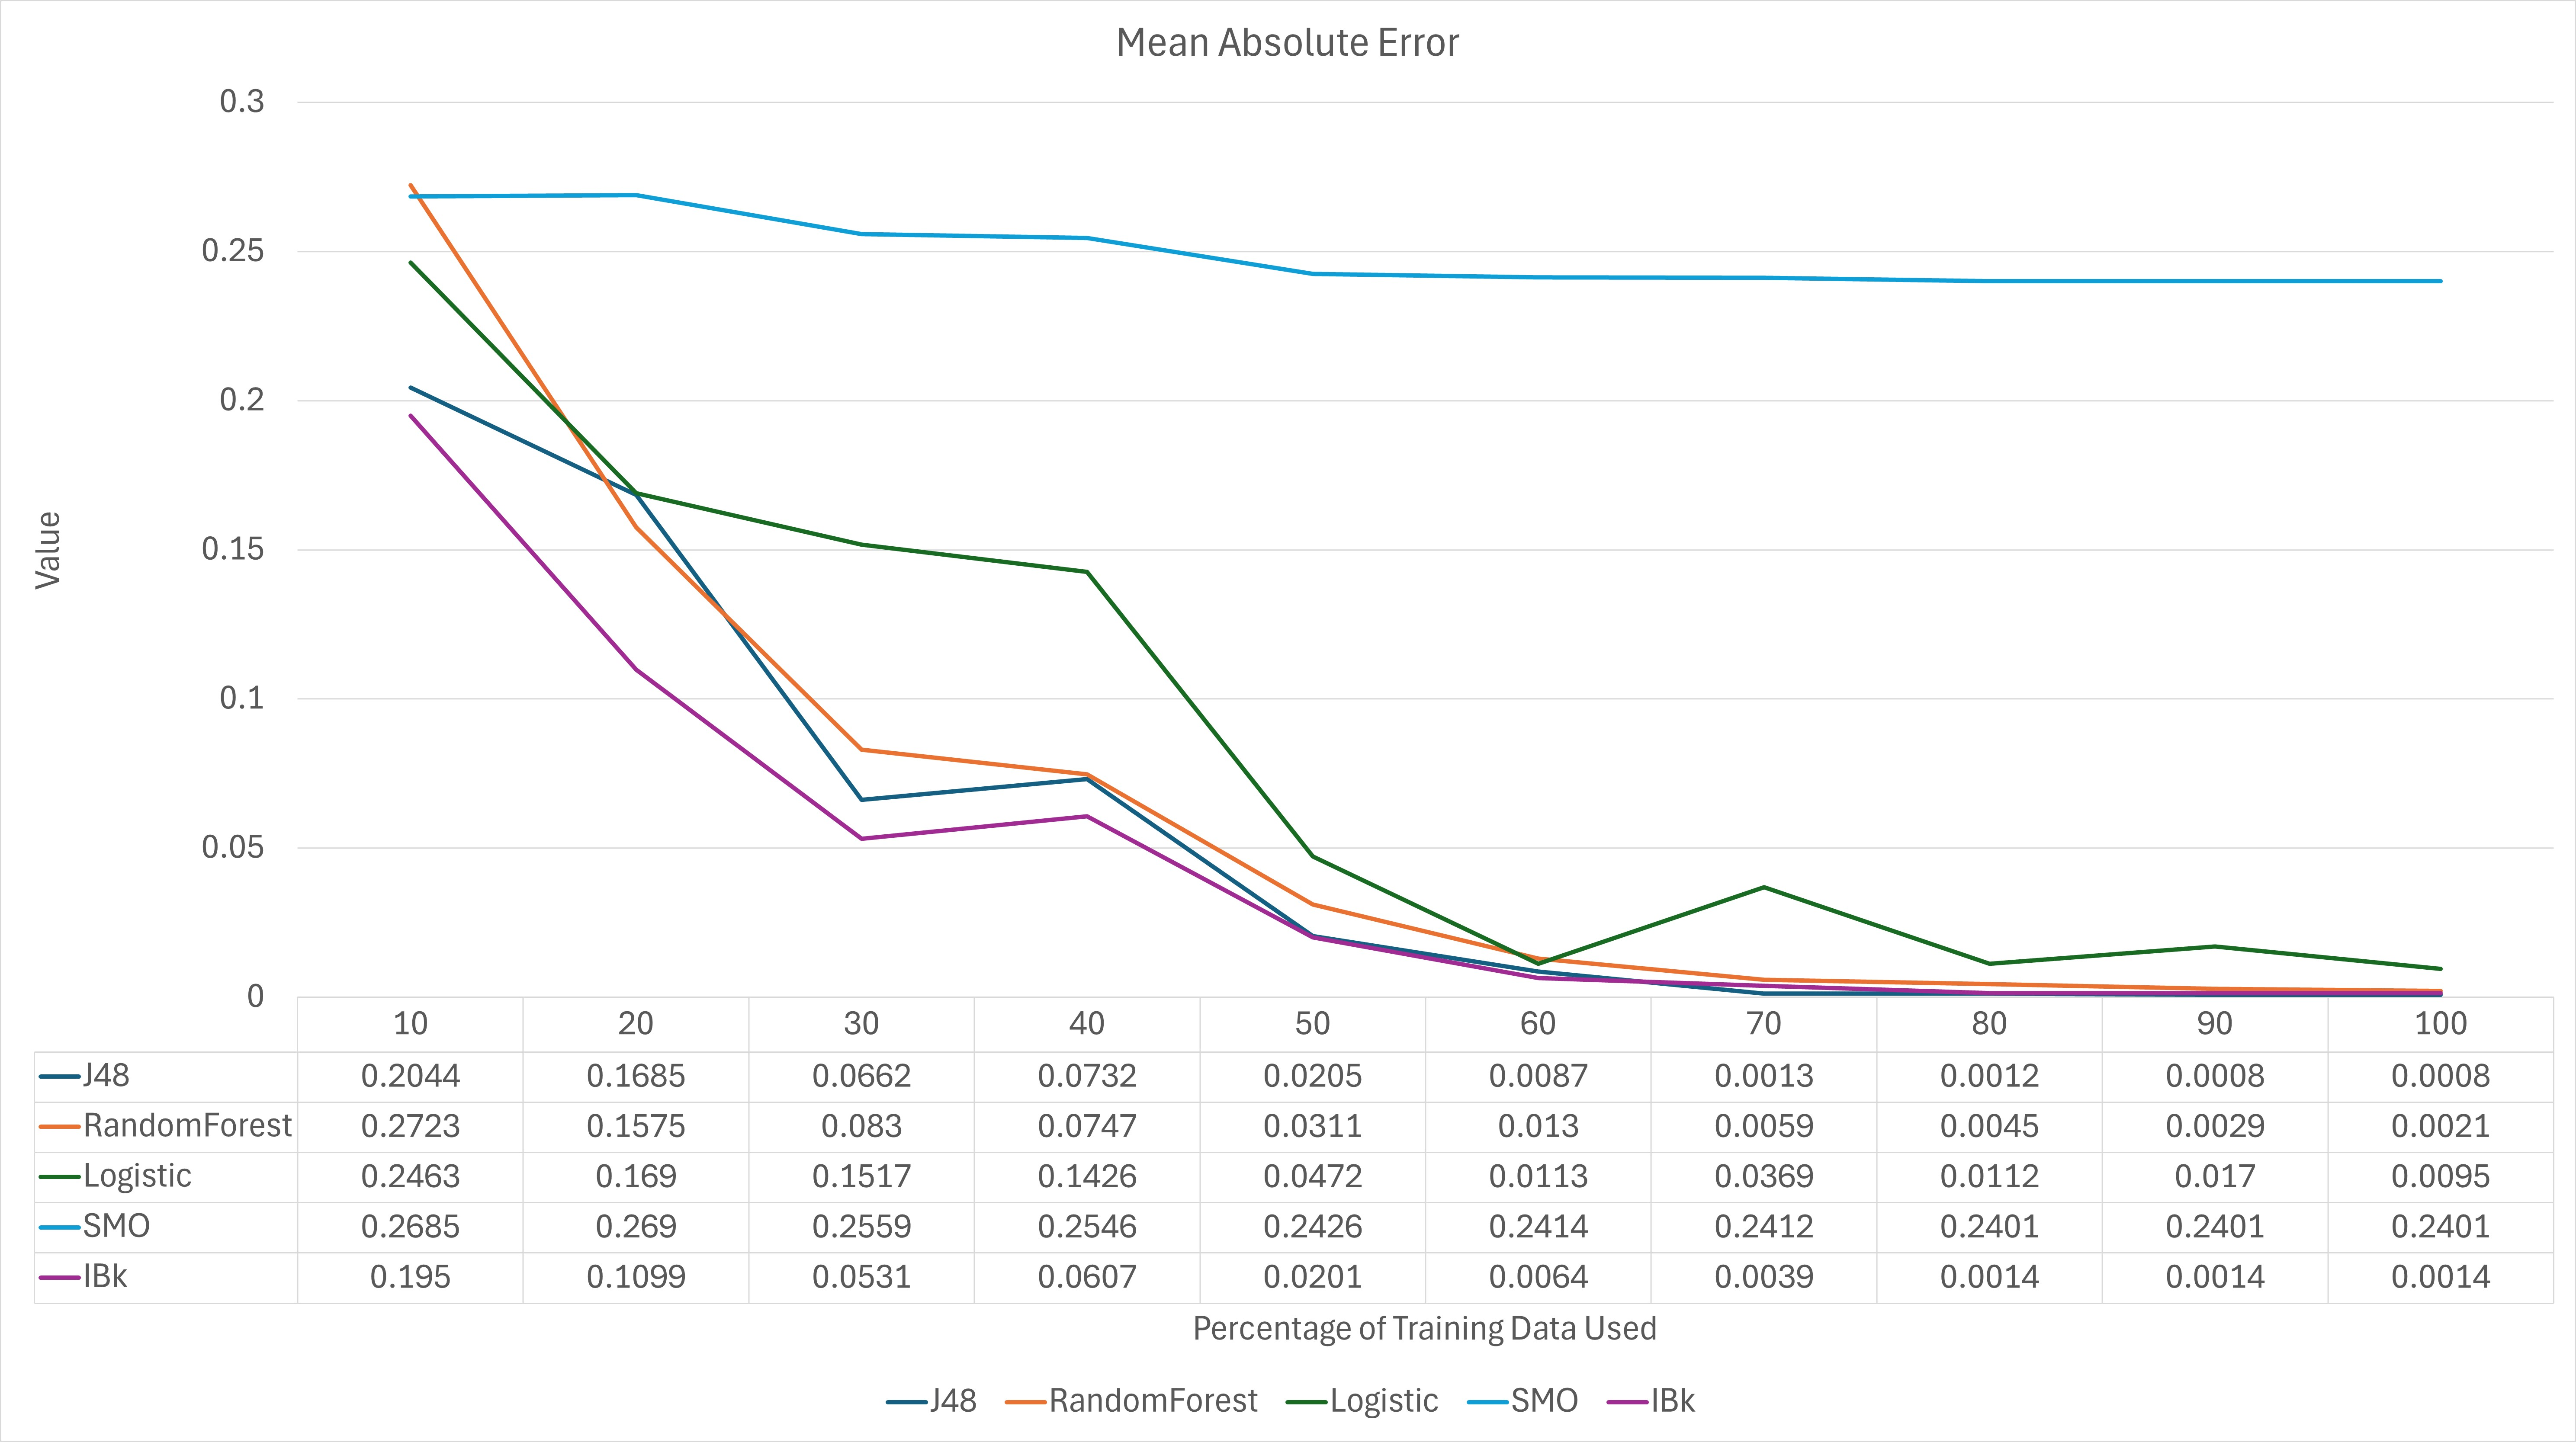
\includegraphics[width=0.9\linewidth]{imagens/figure34.jpg}\label{cap-5-fig34}
    \captionof{figure}[LOF entry]{Comparação da evolução do \textit{Mean Absolute Error}, para cada \textit{training split}.}
    \label{fig34}
    \end{centering}
\end{figure}

O gráfico acima representa a evolução do chamado \textit{\textbf{Mean Absolute Error}}. Esta métrica de erro é utilizada para medir a média das diferenças absolutas entre a classe prevista e a atual. Observando o gráfico, verificamos o seguinte:

\begin{enumerate}
	\item \textbf{\textit{J48}}: O classificador \textit{\textbf{J48}} apresenta valores próximos do \textbf{\textit{Random Forest}} (ambas as linhas do gráfico aparentam seguir percursos similares para cada classificador). Com a utilização de conjuntos de dados de treino progressivamente superiores, o erro medido foi diminuindo, até atingir o seu planalto a partir da utilização de 90\% do conjunto de treino.
	\item \textbf{\textit{Random Forest}}: O classificador \textit{\textbf{Random Forest}} apresentou valores de erro muito promissores, caindo de forma acentuada até cerca dos 60\% do conjunto de treino. Embora os ganhos de redução de erro sejam cada vez menos expressivos com a utilização de maiores conjuntos de treino, o classificador conseguiu atingir o terceiro melhor resultado de entre os restantes.
	\item \textbf{\textit{Logistic}}: O classificador \textit{\textbf{Logistic}} manteve de forma consistente valores de erro superiores à maioria dos restantes algoritmos, mostrando as suas limitações na captura de relações não lineares nos dados.
	\item \textbf{\textit{SMO}}: O classificador \textbf{\textit{SMO}} mantém valores moderados de \textit{Mean Absolute Error} ao longo de todos os testes com diferentes conjuntos de treino, não melhorando tanto como os outros algoritmos.
	\item \textbf{\textit{IBk}}: O classificador \textit{\textbf{IBk}} apresentou os valores de \textit{Mean Absolute Error} mais baixos, mesmo com conjuntos de treino mais pequenos, demonstrando mais uma vez ser um classificador robusto.
\end{enumerate}


\begin{figure}[H]
    \begin{centering}
    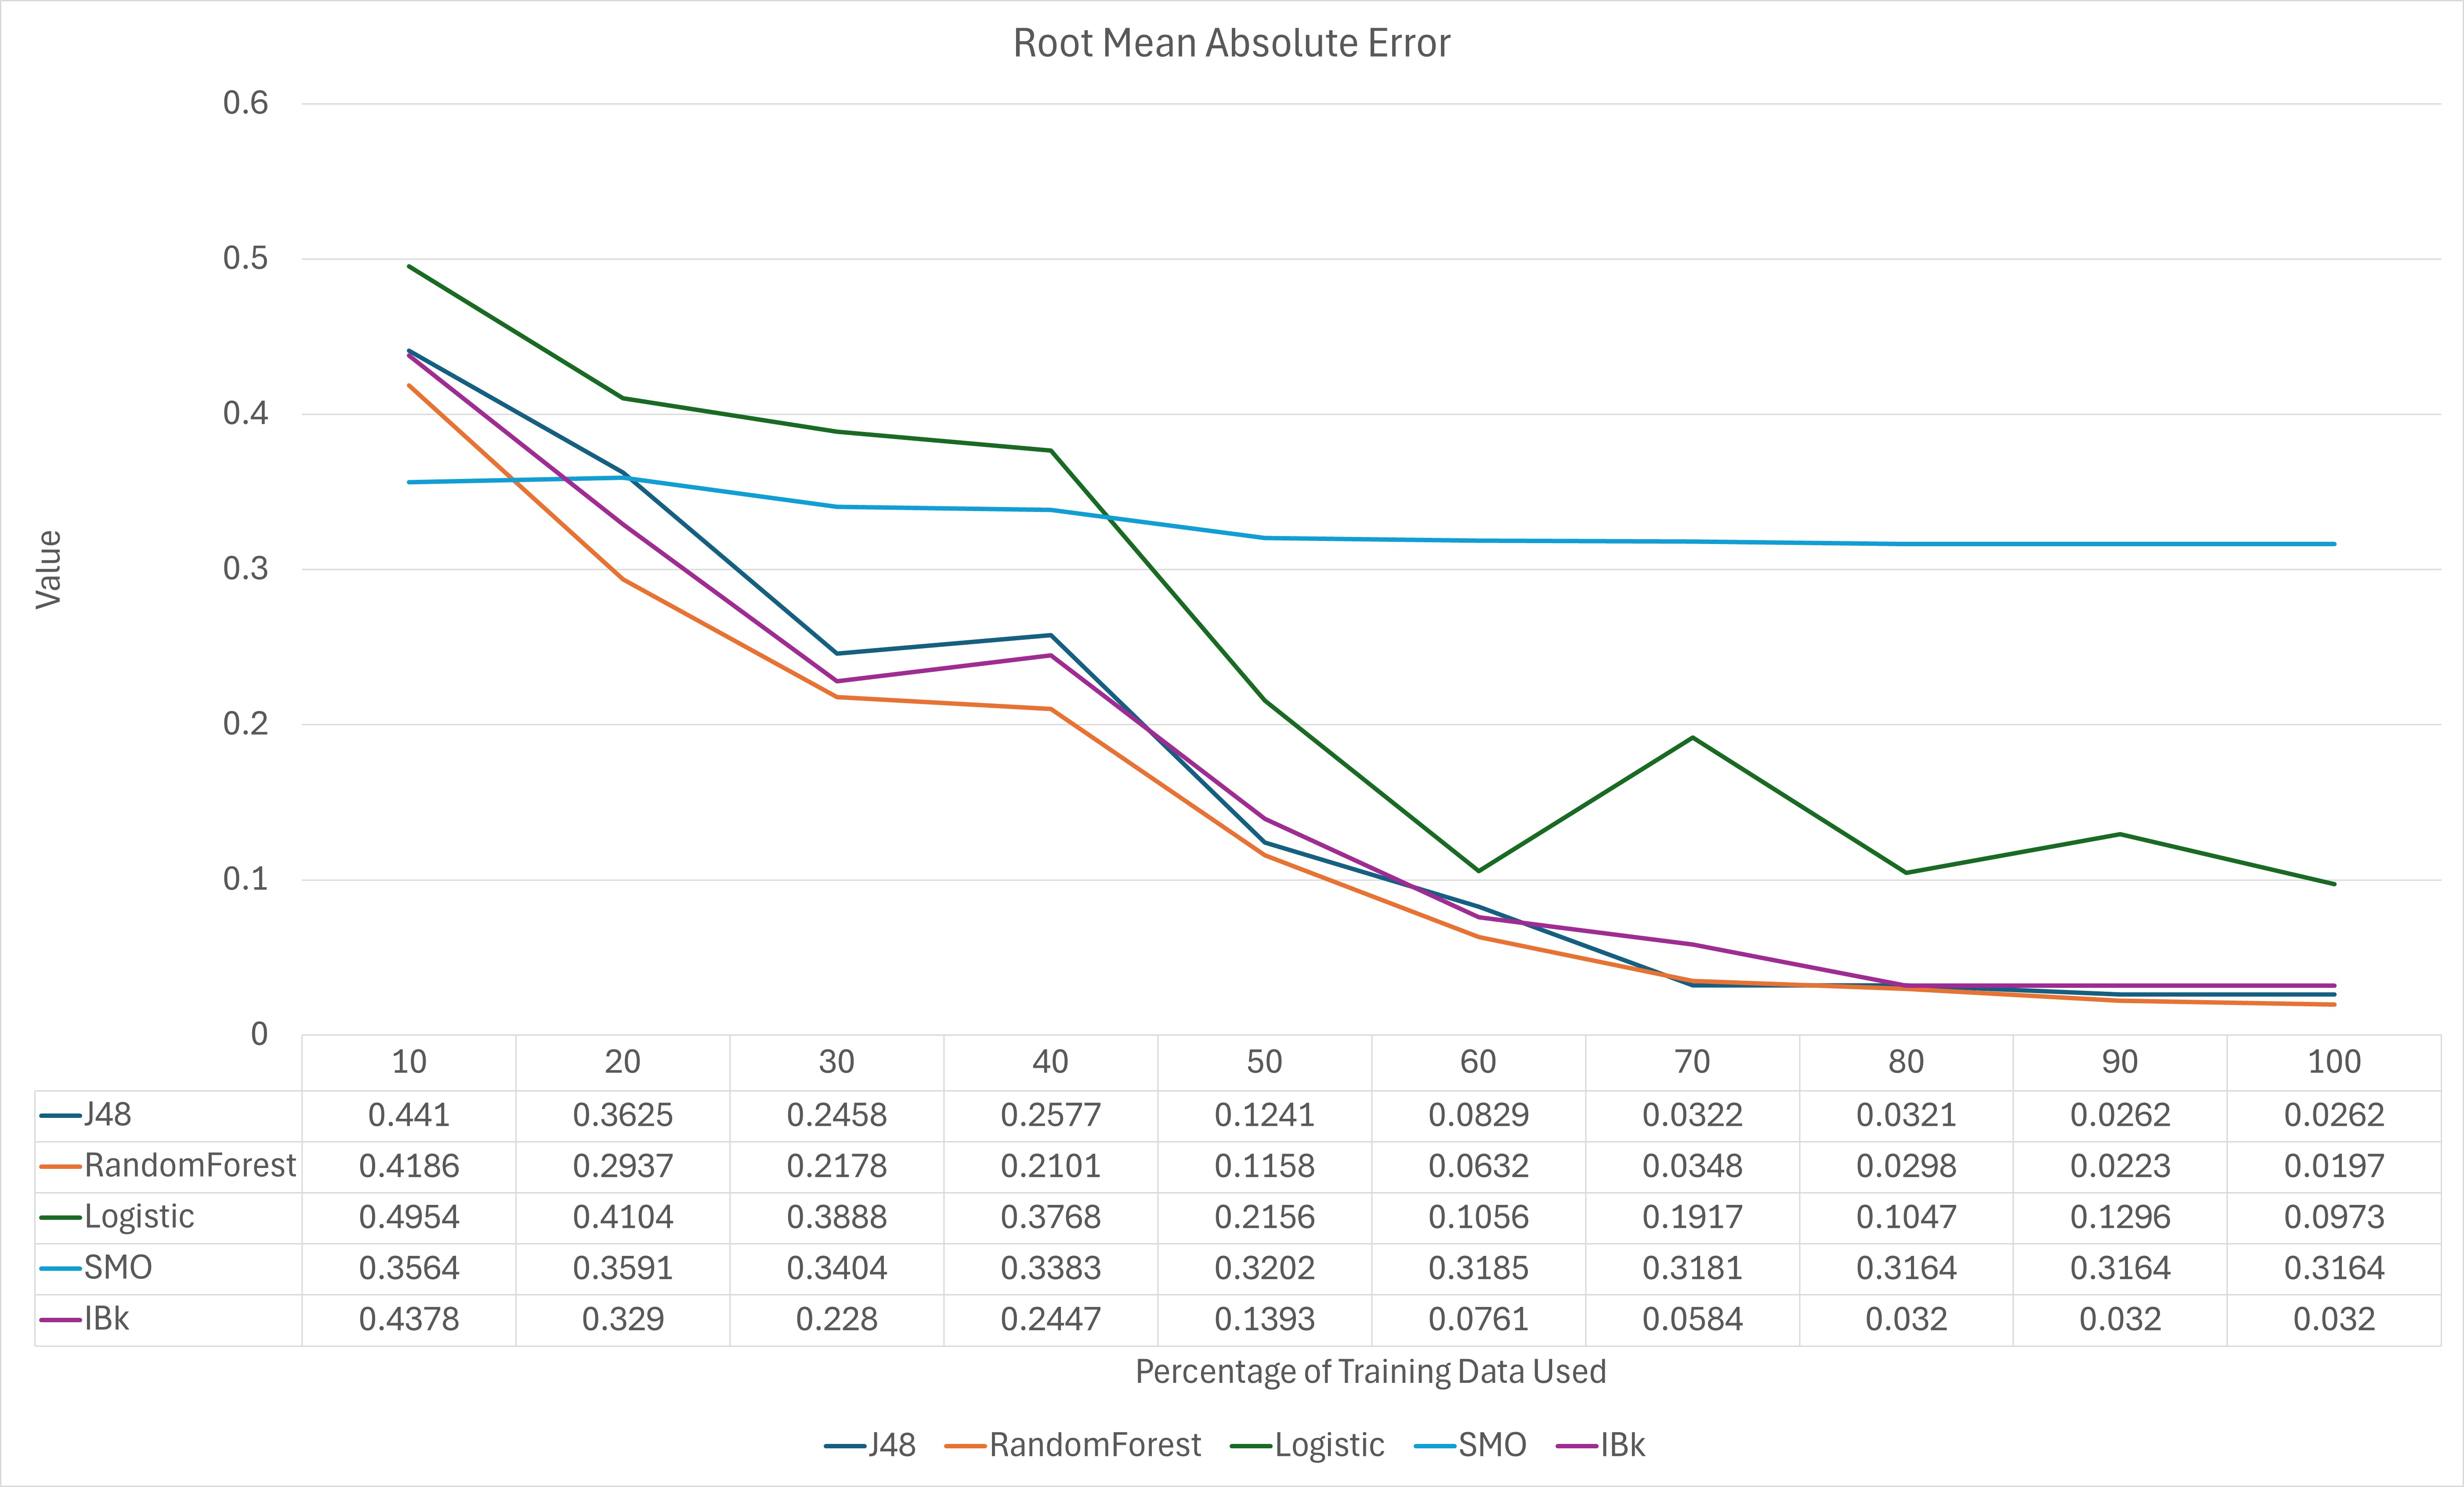
\includegraphics[width=1\linewidth]{imagens/figure35.jpg}\label{cap-5-fig35}
    \captionof{figure}[LOF entry]{Comparação da evolução do \textit{Root Mean Absolute Error}, para cada \textit{training split}.}
    \label{fig35}
    \end{centering}
\end{figure}

O gráfico acima representa a evolução do chamado \textit{\textbf{Root Mean Absolute Error}}. Esta métrica de erro combina a média dos erros absolutos, realizando a sua raiz quadrada. Com esse cálculo é fornecida uma medida balanceada acerca da precisão das previsões, em que valores mais pequenos indicam melhor desempenho. Observando o gráfico, verificamos o seguinte:

\begin{enumerate}
	\item \textbf{\textit{J48}}: O classificador \textit{\textbf{J48}} apresenta valores de \textit{\textbf{Root Mean Absolute Error}} muito próximos do \textit{\textbf{Random Forest}}, sofrendo reduções substanciais à medida que se vão utilizando conjuntos de treino maiores. Atingiu o seu planalto aos 90\% do conjunto de treino.
	\item \textbf{\textit{Random Forest}}: O classificador \textit{\textbf{Random Forest}} apresentou os valores de erro mais baixos, com cada conjunto de treino cada vez maior a contribuir para uma grande redução nos valores desta métrica.
	\item \textbf{\textit{Logistic}}: O classificador \textit{\textbf{Logistic}}, embora valores cada vez maiores do conjunto de treino tenham permitido reduzir o erro associado, manteve-se como um dos piores classificadores, sendo que apenas o \textbf{\textit{SMO}} teve valores de erro superiores.
	\item \textbf{\textit{SMO}}: O classificador \textbf{\textit{SMO}} manteve valores semelhantes de erro ao longo de todos os testes com conjuntos de treino cada vez mais superiores, atingindo o seu planalto aos 80\% do conjunto de treino.
	\item \textbf{\textit{IBk}}: O classificador \textit{\textbf{IBk}} apresentou os valores de \textit{Root Mean Absolute Error} similares ao \textbf{\textit{J48}}, no entanto, atingiu o seu planalto com a utilização de 80\% do conjunto de treino. 
\end{enumerate}

\begin{figure}[H]
    \begin{centering}
    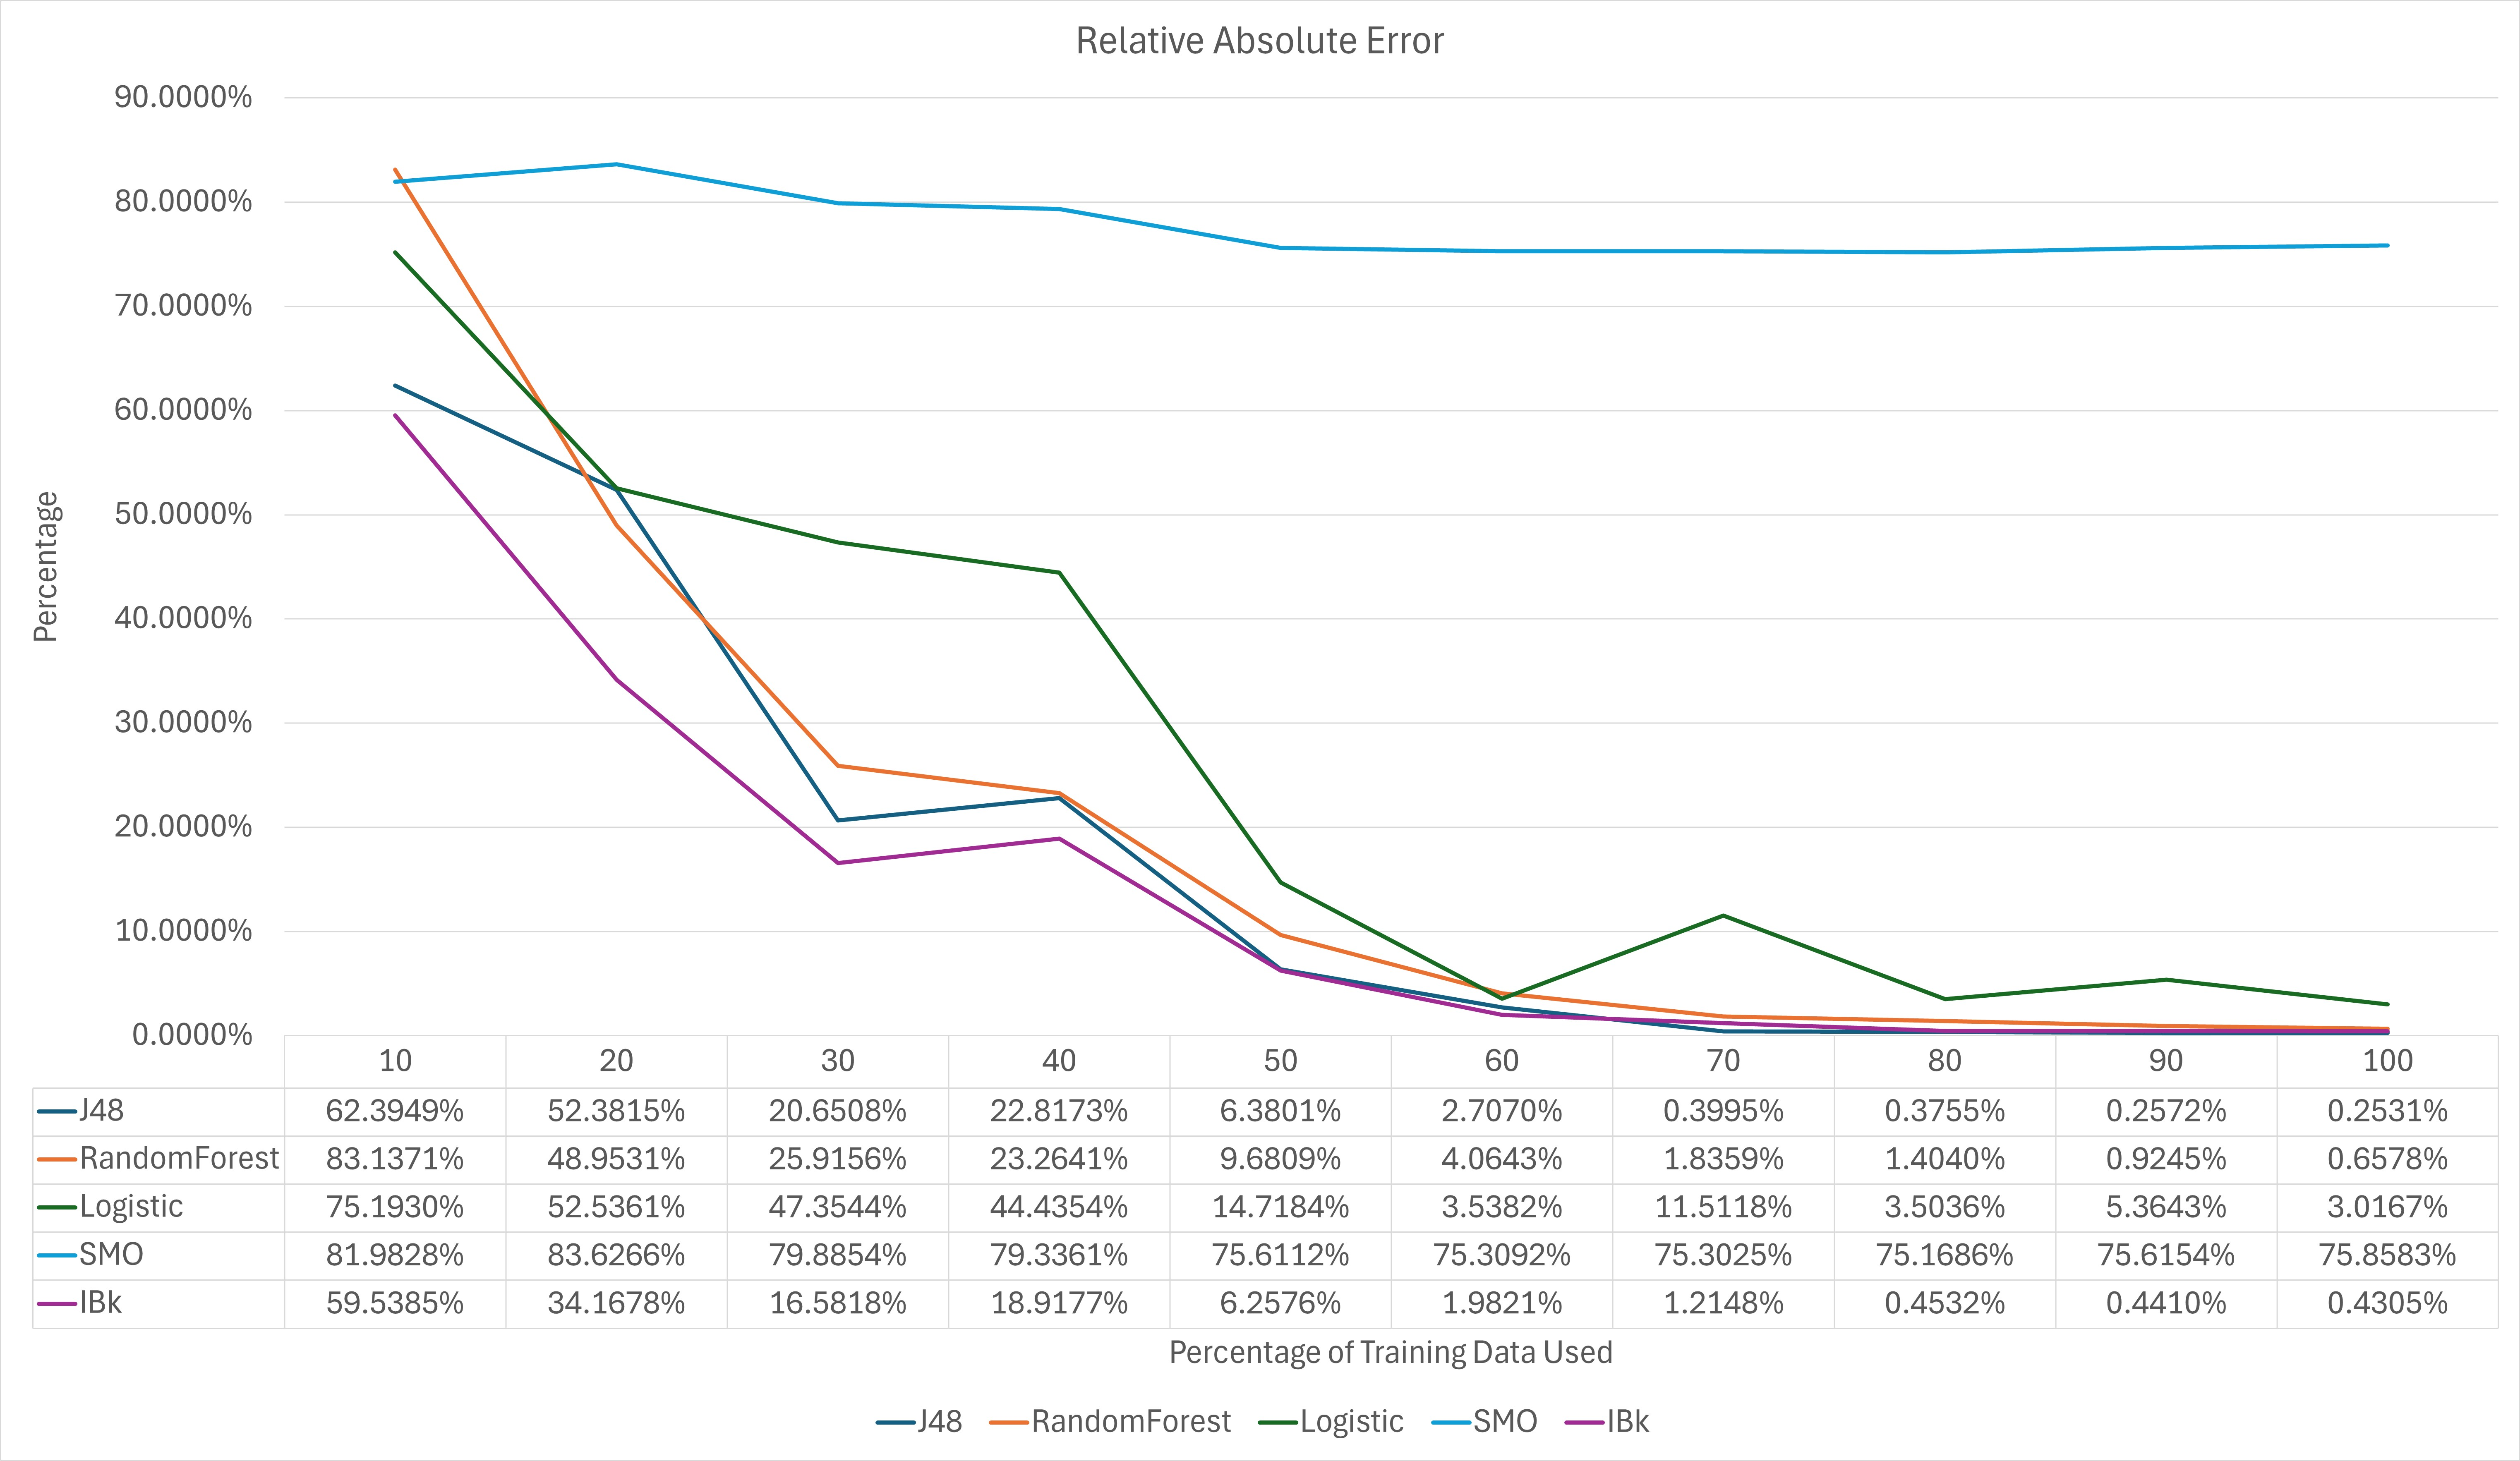
\includegraphics[width=1\linewidth]{imagens/figure36.jpg}\label{cap-5-fig36}
    \captionof{figure}[LOF entry]{Comparação da evolução do \textit{Relative Absolute Error}, para cada \textit{training split}.}
    \label{fig36}
    \end{centering}
\end{figure}

O gráfico acima representa a evolução do chamado \textit{\textbf{Relative Absolute Error}}. Esta métrica de erro avalia como as previsões se desviam dos valores verdadeiros em relação a um modelo ingénuo (através da previsão do valor médio), em que valores inferiores são melhores. Observando o gráfico, reparamos no seguinte:

\begin{enumerate}
	\item \textbf{\textit{J48}}: O classificador \textit{\textbf{J48}} apresenta valores de \textit{\textbf{Relative Absolute Error}} muito próximos do \textit{\textbf{Random Forest}}, tendo atingido o valor mais baixo relativamente aos restantes classificadores.
	\item \textbf{\textit{Random Forest}}: O classificador \textit{\textbf{Random Forest}} apresentou os valores de erro mais baixos, com cada conjunto de treino cada vez maior a contribuir para uma grande redução nos valores desta métrica, desacelerando apenas a partir da utilização de 70\% ou mais do conjunto de treino.
	\item \textbf{\textit{Logistic}}: O classificador \textit{\textbf{Logistic}}, embora valores cada vez maiores do conjunto de treino tenham permitido reduzir o erro associado, esta redução não foi sempre constante, apresentando flutuações. É o segundo pior classificador nesta métrica, sendo apenas superado pelo \textit{\textbf{SMO}}.
	\item \textbf{\textit{SMO}}: O classificador \textbf{\textit{SMO}} apresentou apenas ligeiras reduções dos valores de erro com utilização de conjuntos de treino progressivamente maiores, terminando com o \textit{\textbf{Relative Absolute Error}} mais elevado em relação aos restantes classificadores, por uma grande margem (~75\% no \textbf{\textit{SMO}} \textit{vs.} ~3\% no  \textbf{\textit{Logistic}}).
	\item \textbf{\textit{IBk}}: O classificador \textit{\textbf{IBk}} apresentou uma grande redução nos valores do  \textit{\textbf{Relative Absolute Error}} logo após a utilização de 30\% do conjunto de treino, terminando com a segunda melhor métrica, apenas atrás do \textbf{\textit{J48}}.
\end{enumerate}

\begin{figure}[H]
    \begin{centering}
    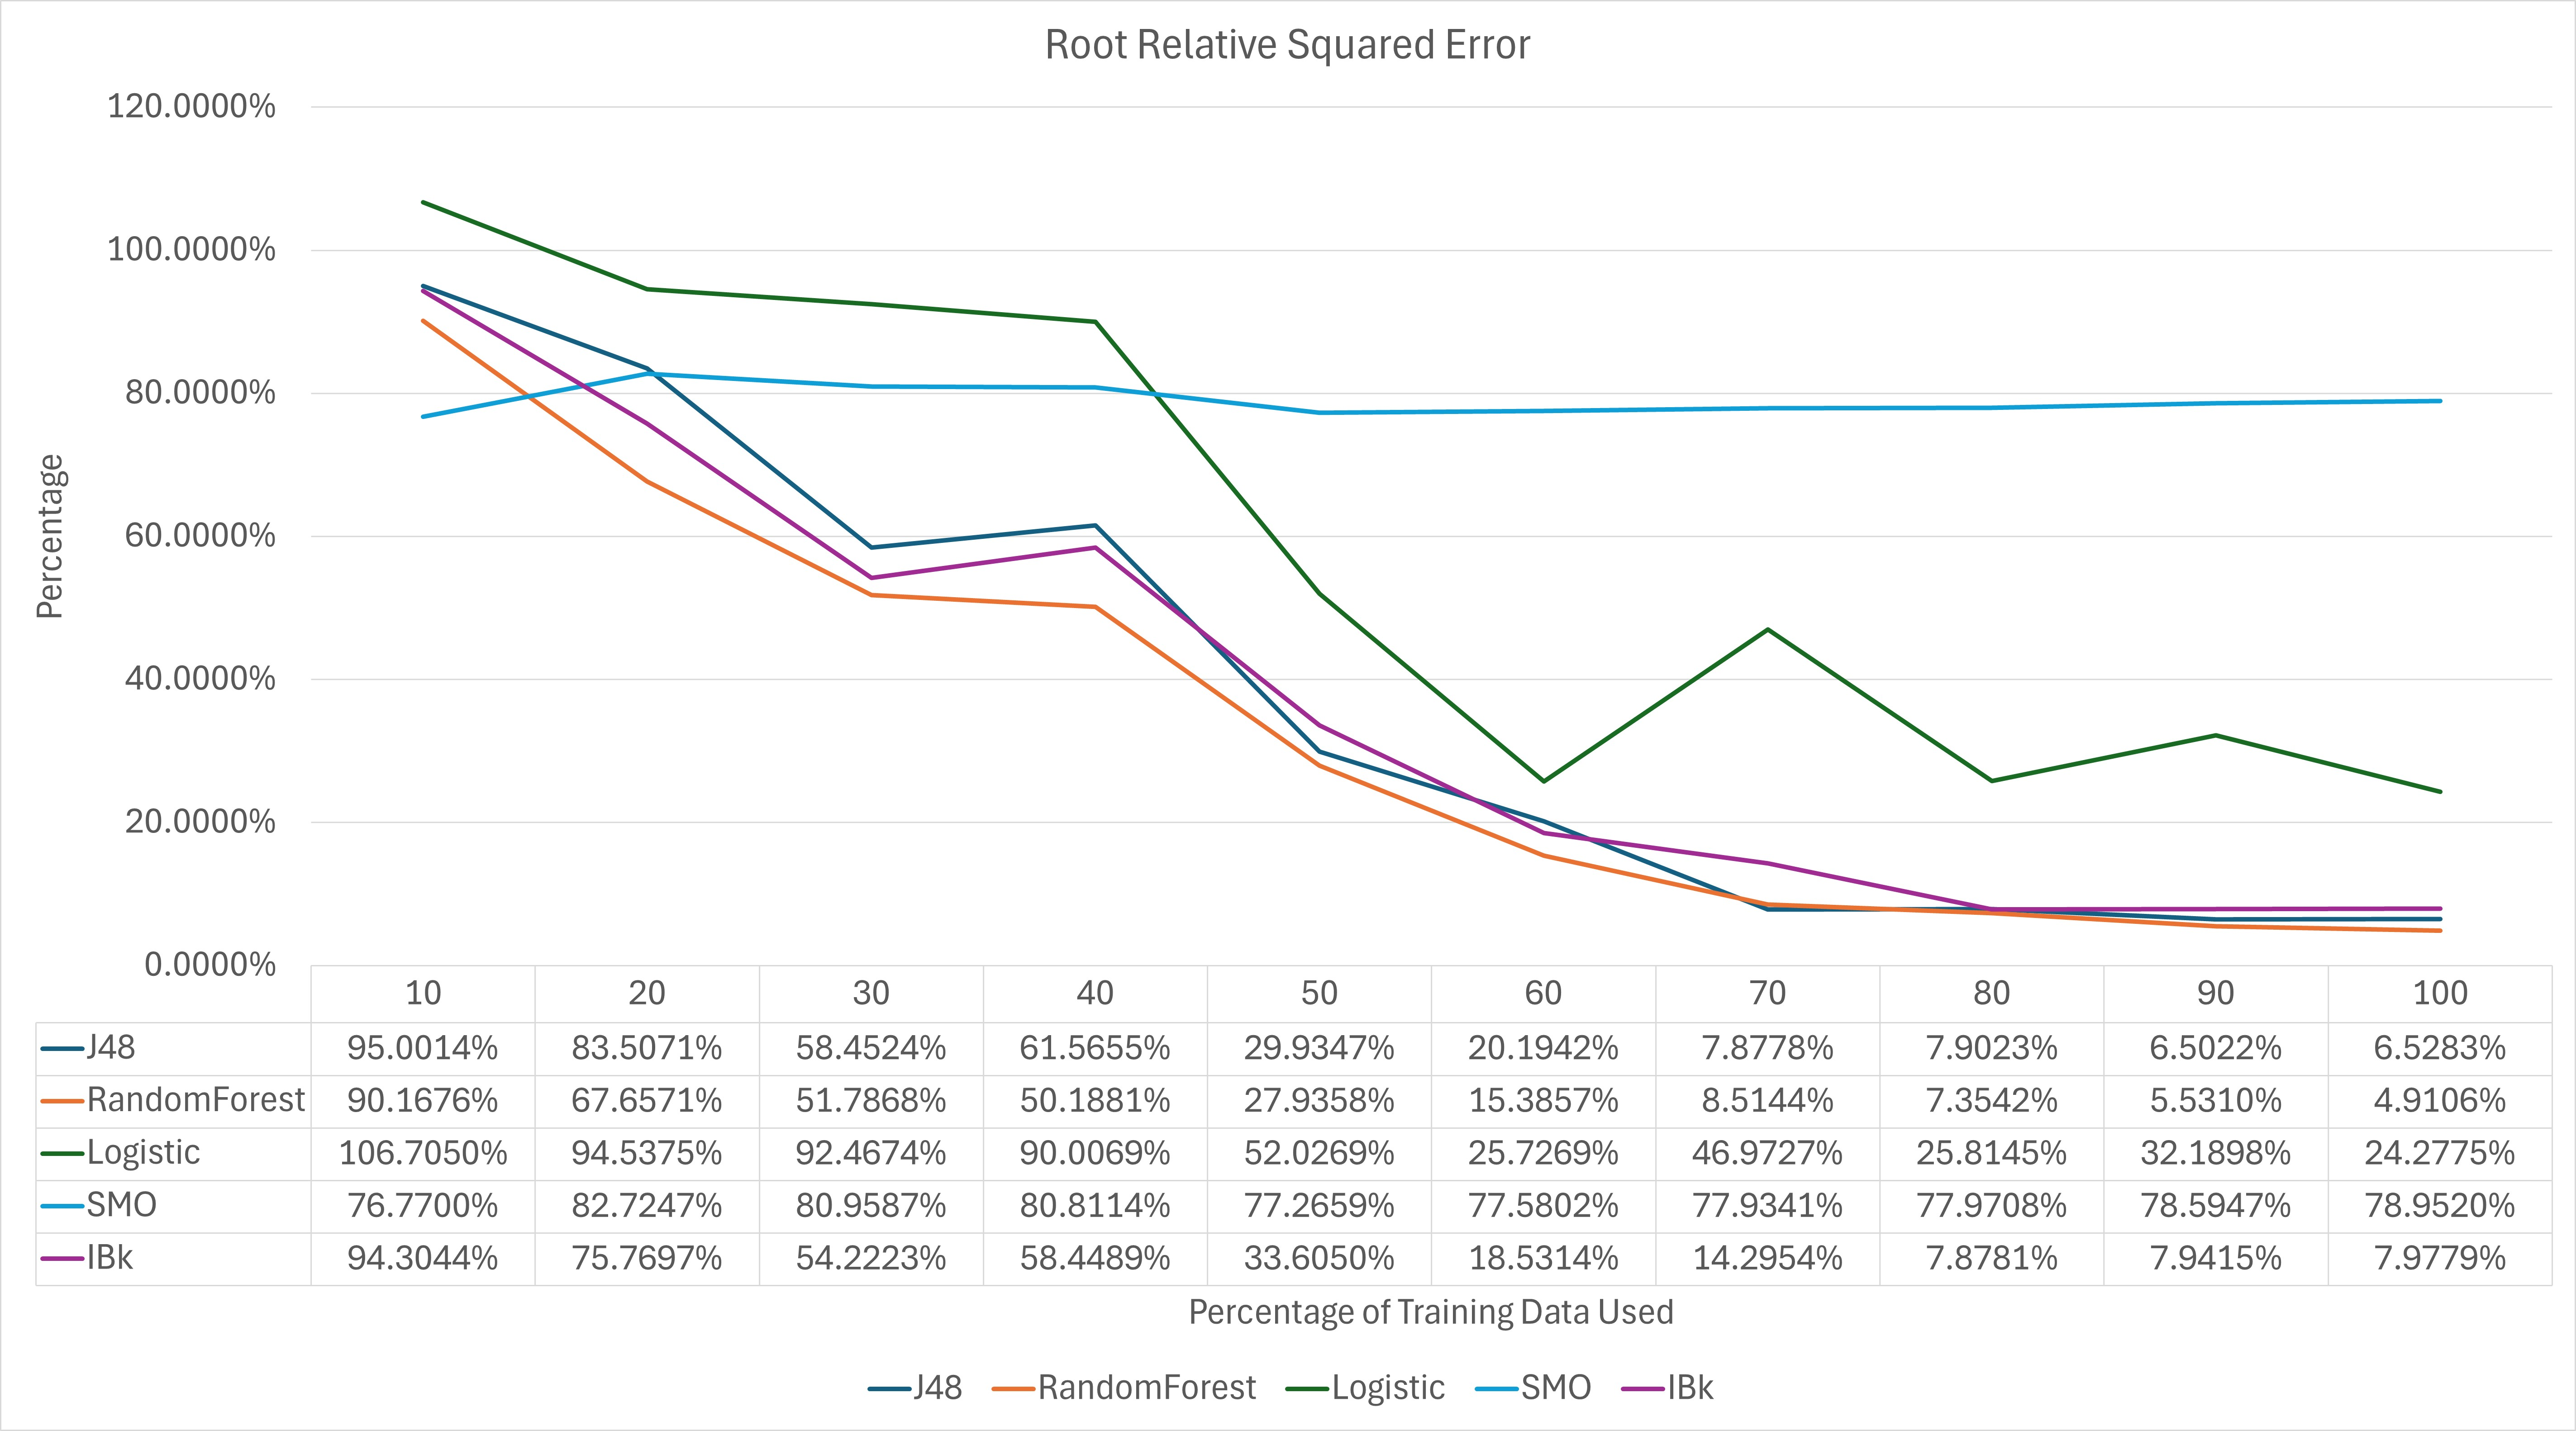
\includegraphics[width=1\linewidth]{imagens/figure37.jpg}\label{cap-5-fig37}
    \captionof{figure}[LOF entry]{Comparação da evolução do \textit{Root Relative Squared Error}, para cada \textit{training split}.}
    \label{fig37}
    \end{centering}
\end{figure}

O gráfico acima representa a evolução do chamado \textit{\textbf{Root Relative Squared Error}}. Esta métrica de erro mede o quadrado dos erros relativos, quando comparados com o valor médio, sendo normalizado pelos valores verdadeiros, com valores menores a indicar melhores resultados. Observando o gráfico, verificamos o seguinte:

\begin{enumerate}
	\item \textbf{\textit{J48}}: O classificador \textit{\textbf{J48}} apresentou bom desempenho na redução do erro, com uma queda acentuada a partir da utilização de 50\% do conjunto de treino. A partir dos 70\% do conjunto de treino, apresentou resultados comparáveis com \textbf{\textit{Random Forest}}.
	\item \textbf{\textit{Random Forest}}: O classificador \textit{\textbf{Random Forest}} apresentou os valores de erro mais baixos, com cada conjunto de treino cada vez maior a contribuir para uma grande redução nos valores desta métrica, desacelerando apenas a partir da utilização de 70\% ou mais do conjunto de treino.
	\item \textbf{\textit{Logistic}}: O classificador \textit{\textbf{Logistic}}, foi apresentando flutuações nos valores de erro com a utilização progressiva de maiores conjuntos de treino. É o segundo pior classificador nesta métrica, sendo apenas superado pelo \textit{\textbf{SMO}}.
	\item \textbf{\textit{SMO}}: O classificador \textbf{\textit{SMO}} apresentou valores um pouco flutuantes no erro em que curiosamente, a partir dos 50\% do conjunto de treino, o erro ia subindo ligeiramente.
	\item \textbf{\textit{IBk}}: O classificador \textit{\textbf{IBk}} apresentou uma grande redução nos valores do  \textit{\textbf{Root Relative Squared Error}}, no entanto após os 80\%, o erro começou a subir ligeiramente.
\end{enumerate}


Observando todas as métricas de erro anteriores, torna-se claro que os algoritmos que apresentaram melhor desempenho foram o \textbf{\textit{Random Forest}} e o \textbf{\textit{IBk}}.

O \textbf{\textit{Random Forest}} atingiu de forma consistente valores de erro muito baixos em todas as métricas e tamanhos de dados de treino, indicando a sua robustez e capacidade na modelação de relações complexas entre dados.

O \textbf{\textit{IBk}} também atingiu de forma consistente valores de erro muito baixos em todas as métricas e tamanhos de dados de treino, no entanto demonstrou ser particularmente eficaz quando foram utilizados conjuntos de dados mais pequenos, o que indica que é uma boa escolha para cenários onde os dados de treino têm dimensão limitada.

O \textbf{\textit{Logistic}} exibiu valores de erro flutuantes e inconsistentes em todas as métricas e tamanhos de dados de treino, o que, embora tenha atingido valores de desempenho altos quando utilizados conjuntos de treino maiores, demonstra as suas dificuldades em capturar e modelar relações não lineares entre os dados.

O \textbf{\textit{J48}} obteve resultados muito semelhantes ao \textbf{\textit{Random Forest}}, com a vantagem das suas regras serem interpretáveis. No entanto, para tarefas que necessitem do maior desempenho possível, o \textbf{\textit{Random Forest}} é sempre melhor escolha.

\section{Conclusão e trabalho futuro}
A análise RFM combinada com técnicas de mineração de dados mostrou-se uma ferramenta poderosa para segmentação de clientes e previsão do risco de abandono em contextos de \textit{e-commerce}. Este estudo permitiu identificar e categorizar os clientes com base em métricas claras de \textbf{Recência}, \textbf{Frequência} e \textbf{Valor Monetário}, possibilitando uma melhor compreensão dos seus comportamentos e necessidades. Além disso, a normalização das métricas e a aplicação de métodos de \textit{clustering}, como o \textit{K-means}, viabilizaram a criação de segmentos bem definidos, facilitando a implementação de estratégias de retenção e fidelização.

O cálculo do risco de abandono, baseado em uma abordagem ponderada das métricas RFM, destacou-se como um indicador valioso para orientar ações personalizadas de \textit{engagement}. A visualização tridimensional dos dados reforçou a importância de estratégias adaptativas, focadas nos diferentes perfis de clientes, desde os mais valiosos e leais até aqueles em risco de inatividade.

Embora os resultados obtidos sejam promissores, é importante ressaltar que o modelo utilizado neste estudo está limitado à análise de métricas RFM. Para alcançar previsões mais robustas e abrangentes, recomenda-se a inclusão de dados adicionais, como características demográficas, socioeconômicas e comportamentais.

Este trabalho reforça a importância do uso de abordagens baseadas em dados no cenário competitivo atual, oferecendo uma base sólida para a criação de estratégias centradas no cliente. A replicabilidade dos métodos apresentados torna-os aplicáveis a diferentes contextos empresariais, sendo uma valiosa contribuição para a gestão e análise de clientes.

Embora este estudo tenha demonstrado a eficácia da análise RFM e da segmentação de clientes baseada em \textit{clustering} para a identificação de padrões de comportamento e prever o risco de abandono, há diversas oportunidades para melhorias e extensões futuras. Uma das extensões futuras para este trabalho, seria a expansão da análise para estudar as tendências dos clientes ao longo do tempo, com o uso de séries temporais, para fornecer \textit{insights} mais profundos sobre o comportamento e a evolução do risco de abandono. Este processo já foi de certa forma explorado no artigo \textit{"Predicting Customer Profitability over time based on RFM time series"} da autoria de \textit{Daqing Chen}, \textit{Kun Guo} e \textit{George Ubakanma}, mas o foco da sua análise foi o estudo da rentabilidade de clientes ao longo do tempo, em vez da evolução do risco de abandono. Como tal, a evolução do risco de abandono ao longo do tempo apresenta-se como um bom candidato para exploração futura, dado o número limitado de artigos e pesquisa desenvolvida sobre esse tema.

\newpage
%----------------------------------------------------------------------------------------------------------
\bibliographystyle{plain}
\bibliography{artigo}

\end{document}